\documentclass[dvipdfmx]{jreport}
% \usepackage{graphicx}
\usepackage[dvipdfmx]{graphicx}
\usepackage{sty/masterthesis}
%\usepackage{showkeys}%推敲用
\usepackage{lscape}	%横
\usepackage{mathptmx} % Timesへ
\usepackage{comment}
%\usepackage{booktabs}  %表結合
%\usepackage{multirow}  %表結合
%\usepackage{sty/slashbox}   %斜線
\usepackage{dcolumn}
\usepackage{array}
\usepackage{here}
\usepackage{enumerate}
\pagestyle{plain}
\makeatletter
\def\@cite#1{$\m@th^{\hbox{\@ove@rcfont #1)}}$} 
\def\@biblabel#1{[#1]}                              %参考文献[]へ
\def\@cite#1{{\mbox{\scriptsize{[#1}]}}}            %参考文献[]を文右へ
\makeatother
\setcounter{tocdepth}{2}                            % サブセクションも目次に出力
\begin{document}

%----------------------------------------------------------------------
% 表紙(年度,邦文題目,英文題目,指導教員,氏名,学籍番号を記入)
% ※題目には適宜改行(\\)を手動で入れる
%----------------------------------------------------------------------
\年度{2023}
\邦文題目{「人馬一体感」に向けて意識的に行う身体動作のデザインに関する考察:手指の構造変換を伴う体験型作品《Grasp(er)》を通じて}
\英文題目{A Study on the Design of Conscious Body Movements Toward Sense of  ``''\textit{Jinba Ittai}'': Through ``Grasp(er)'', an Experiential Artwork with Hand-Finger Structure Transformation}
\指導教員{小林 茂, 桑久保 亮太, 平林 真実}
\氏名{山岸 奏大}
\学籍番号{22117}
% \表紙出力

\input{contents/prologue.tex}
\newpage

%----------------------------------------------------------------------
% 目次
%----------------------------------------------------------------------
\contents

% 付図・付表のリストを作成する
\appendixpage{1}

%---------------------------------------------------------------------
% 1章 序論
%----------------------------------------------------------------------
\chapter{はじめに}
\label{introduction}

\section{研究背景}
\label{subject}
``Embodiment''という言葉が、心理学やロボティクス、バーチャルリアリティ(VR)、ヒューマンインターフェースデザインなど、さまざまな分野で注目されている。Botvinick \& Cohenによるラバーハンド錯覚\cite{BotvinickCohen1998}の報告は、私たちが自分の身体として認知する対象は生まれ持った肉体に限らないことを示した。それを皮切りに、「私たちはどこまでを自分の身体として認識しうるか?」、すなわち「何を``身体化''できるのか?」について、その可能性と限界を探る研究が次々と発表されている。また、インターフェース研究者の渡邊は「まさに自分自身の身体である」という感覚を指すGallagherの``sense of ownership''を「自己帰属感」と訳し、インターフェースにおける直感操作を実現する重要な指針として、「身体化」の議論との橋渡しをした。

Embodimentの訳は「身体化、一体化、身体性」など文脈によって異なるが、これらについては「身体化」と訳すことが適当だと思われる。そして、「``身体化''としてのembodiment」は、人間の可能性の拡張や、より直感的で便利な人と道具の関係性を実現するためのデザインへの応用へと広がっている。

% インターフェース研究者の渡邊は、インターフェース設計における理想形を「透明化」であると説明する\cite{Watanabe2017}。すなわち、どんなに複雑で高度な道具であっても、原始的な道具のように原因と結果の関係が直接的であり、道具そのものに対して意識することなくそれを使用できることこそが理想とした。

% そして渡邊は、その理想を実現するための重要な指針が「自己帰属感(sense of ownership)」であると提言する。自己帰属感とは、「あたかもその装置が身体の延長であるかのように感じられる」感覚を指す。

% 人々を取り巻くものが機械や情報処理によって高度化する中、人々と機械との接点を設計することが重要となった。
% ここで、人々と機械との最適な関係を「より使いやすく有用に」\footnote{国際標準化機構(ISO)による「人間中心設計」の導入部\cite{hcd}より}することとし、それを具現化してきたのがエルゴノミクス、人間中心設計といった設計論である。

% 道具の使用における行為と結果の関係から捉えたとき、「使いやすさ」とは、原始的な道具のように直接的であり、道具そのもに対する意識がなくなっていく「透明化」を指す。

% 渡邊は、その理想を実現する指針として「自己帰属感」という概念を導入し、例えばマウスカーソルやスマートフォンのような「操作時の指とグラフィックの追従性が高い」インターフェースは自身の一部や延長として感じられる、「透明」なインターフェースであると説明する。

% こうした設計論は、確かに複雑で高度な道具の力を借りて人間の活動の可能性を拡げることに貢献してきた。
しかし、これらの議論だけでは、embodimentについて見落とされている側面があるのではないだろうか。上記でみてきたembodimentは、「私たちの身体に帰属する他者」という関係性だった。ここではその逆の、「他者に帰属する私たち」という関係性について考えてみたい。例えばそれは、ピアノと人との間に生起する。ピアノを初めて弾くとき、奏者は手の大きさによる制約を受け、最初のうちは左右別々に指を動かすだけでも困難さを経験する。しかし、試行錯誤を経て、ピアノの制約と自身の身体能力との間で折り合いをつけていくことで、ようやく楽器を通して表現ができるようになる。ミュージシャンのスキャットマン・ジョン(ジョン・ポール・ラーキン)は、「吃音症」という発話障害を抱え、「自身の身体」という切っても切り離せない存在をコントロールできない中、むしろその症状を逆手に取るように「テクノスキャット」という独自の歌唱法を開拓した。こうした方法をとって他者と調和していくことは、上記の議論とは逆向きのembodimentと言えるのではないだろうか。

こうした関係について考えるにあたっては、embodimentを「自己」と「他者」の関係に対して中立的な``一体化''として訳すことが適当だと考える。そして、「自己」と「他者」のあいだで相互に折り合いをつけていくようなこの``一体化''は、そうなるまで過程における困難と、それを克服してうまいやり方を見出していく、高度な人間性の発揮の喜びと、創造性を内在している。

そこで本研究では、こうした双方向的な一体感がその名前に象徴的に現れる「人馬一体」という言葉に注目した。こうした双方向的な一体化のプロセスは、例えば楽器やバイクなどにもみられる。これを具現化するような関係性が芽生える体験は、いかにして設計できるのか。この問いについて、手指の変換表現からアプローチしていく。

% \section{リサーチクエスチョン}
% \label{research_question}
% 前節では、研究背景に触れ、本研究が「人馬一体」と言われるような、相互の折り合いをつけながら生まれる親密さについて探索するものであると説明した。ここでは、探索の上での中心的な問いについて明記する。

% \begin{quote}
% \textbf{対象からの影響も受けつつ、相互の折り合いをつけながら生まれる一体感はどのように生まれるのか。そして、それはいかに設計できるのか。}(最後に回収)
% \end{quote}

% 本研究では、「手指の異なる形状への変換」を通して「身体の中の他者性」を経験させる表現を探索することからこの問いに迫った。

\section{研究概要}
本研究では、手指の異なる形状への変換から「身体の中の他者性」を経験させる表現によって、人馬一体のような「一体感」生起を目指し、探索的なプロトタイピングを行なった。その上で、「``一体化''としてのembodiment」から人と対象との関係を分類したとみられるコンピュータ工学者Sydney Felsの分類を援用し、制作されたプロトタイプから重要だと考えられる表現で構成された修士作品《Grasp(er)》を制作した。本研究の狙いは、この作品の制作と体験の分析を通して「人馬一体感」のデザインの道筋を示すことである。4名の作品体験を振り返ることから、それが実現しているかについて考察する。

\section{「身体の中の他者性」に取り組む動機}
\label{prototyping_concept_making}
本研究は、「人馬一体感」の生起に、手指の異なる形状への変換から「身体の中の他者性」を経験させる表現を通して探索する。この表現から取り組むこととした動機は、もともと抱いていた\ref{subject}節のような問題意識に対して、当初はその問題意識とは無関係に進めていた「動きのスケッチツール」という目的の習作「Digitize」を展示した際の体験者の様子が、その切り口になると捉えたためである。
この節では、その習作について説明し、この表現を通して探索することの動機とする。

「Digitize」とは、手指の動きを別の形へとマッピングさせた3つの変換表現から構成された習作である。静止画について構想を膨らませる際、「紙とペン」を通して直接イメージをスケッチできるが、動きについてもそれに相当するほど、直感的かつ、高い表現力でスケッチができるツールを作ろうとしていた。そこで、動きに関して高い表現力を有する手指の動きを使って、「動きをスケッチする」ツールについて案じていた。しかし手指の動きをそのまま表示するのでは、手指を使うことの意義が薄い。手指は人間の身体の中でもとりわけ随意に、高い表現力で動かすことのできる器官である。もし「手ではない形」を通してでも、様々な形や動きを自由に作れるのなら、人間の身体構造による制約を超えた「動きのスケッチ」ができるのではないか。そうして、手指の動きをトラッキングしつつ、画面上でその動きは別の形へマッピングされて動くインターフェースについて、プロトタイピングを行い、その過程を、2022年7月に岐阜県大垣市で開催されたイベント「IAMAS Open House 2022」にて展示した\footnote{\url{https://k1105.github.io/eee_openhouse_2022/}}。この時点では、動きを記録する機能は存在しておらず、あくまで手と、それに伴って動く手指とは異なる形の動きが確認できるだけのものであった。

\begin{figure}[H]
  \centering
  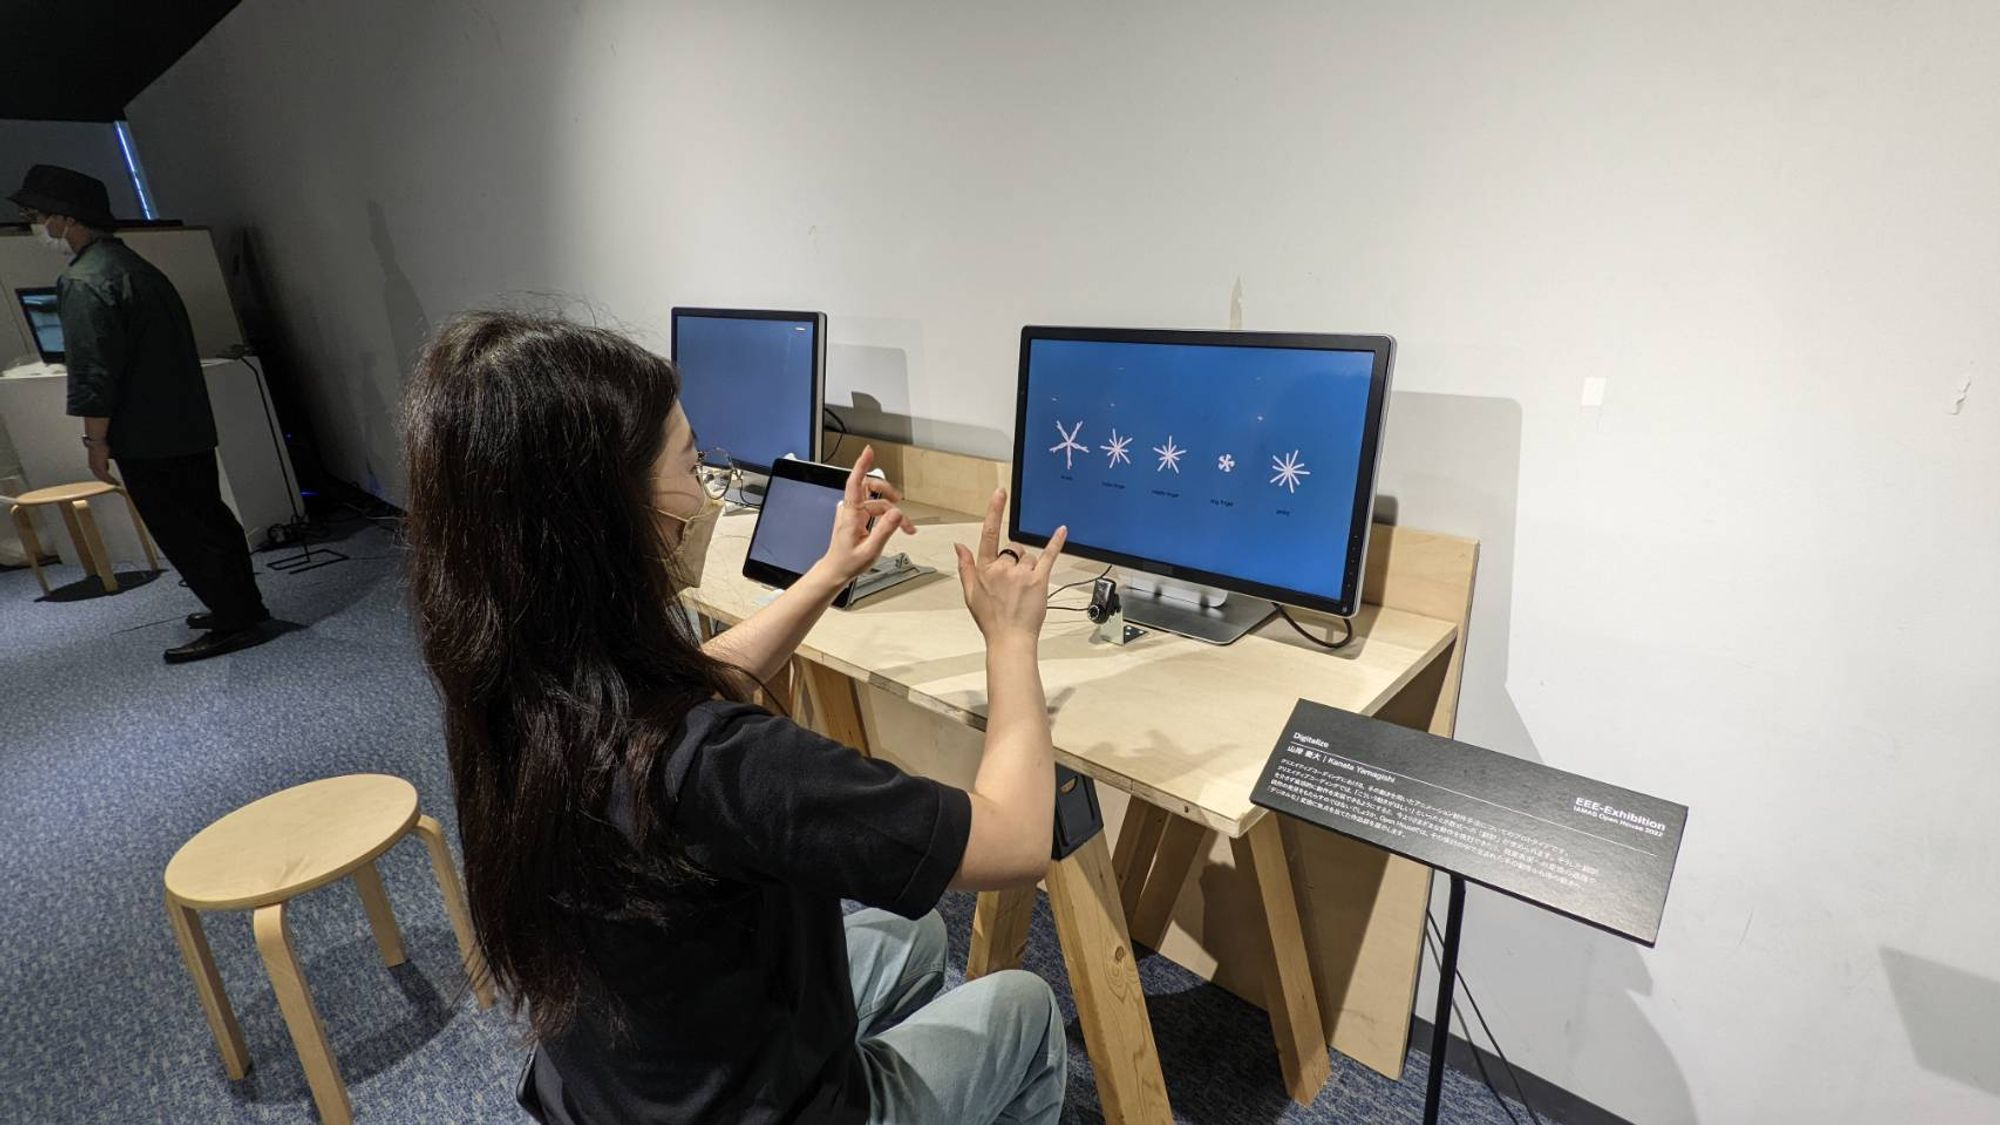
\includegraphics[width=15cm]{img/openhouse2022.jpeg}
  \caption{IAMAS Open House 2022での展示の様子(2022年)}
  \label{fig:exhibit_2022}
\end{figure}

\begin{figure}[H]
  \centering
  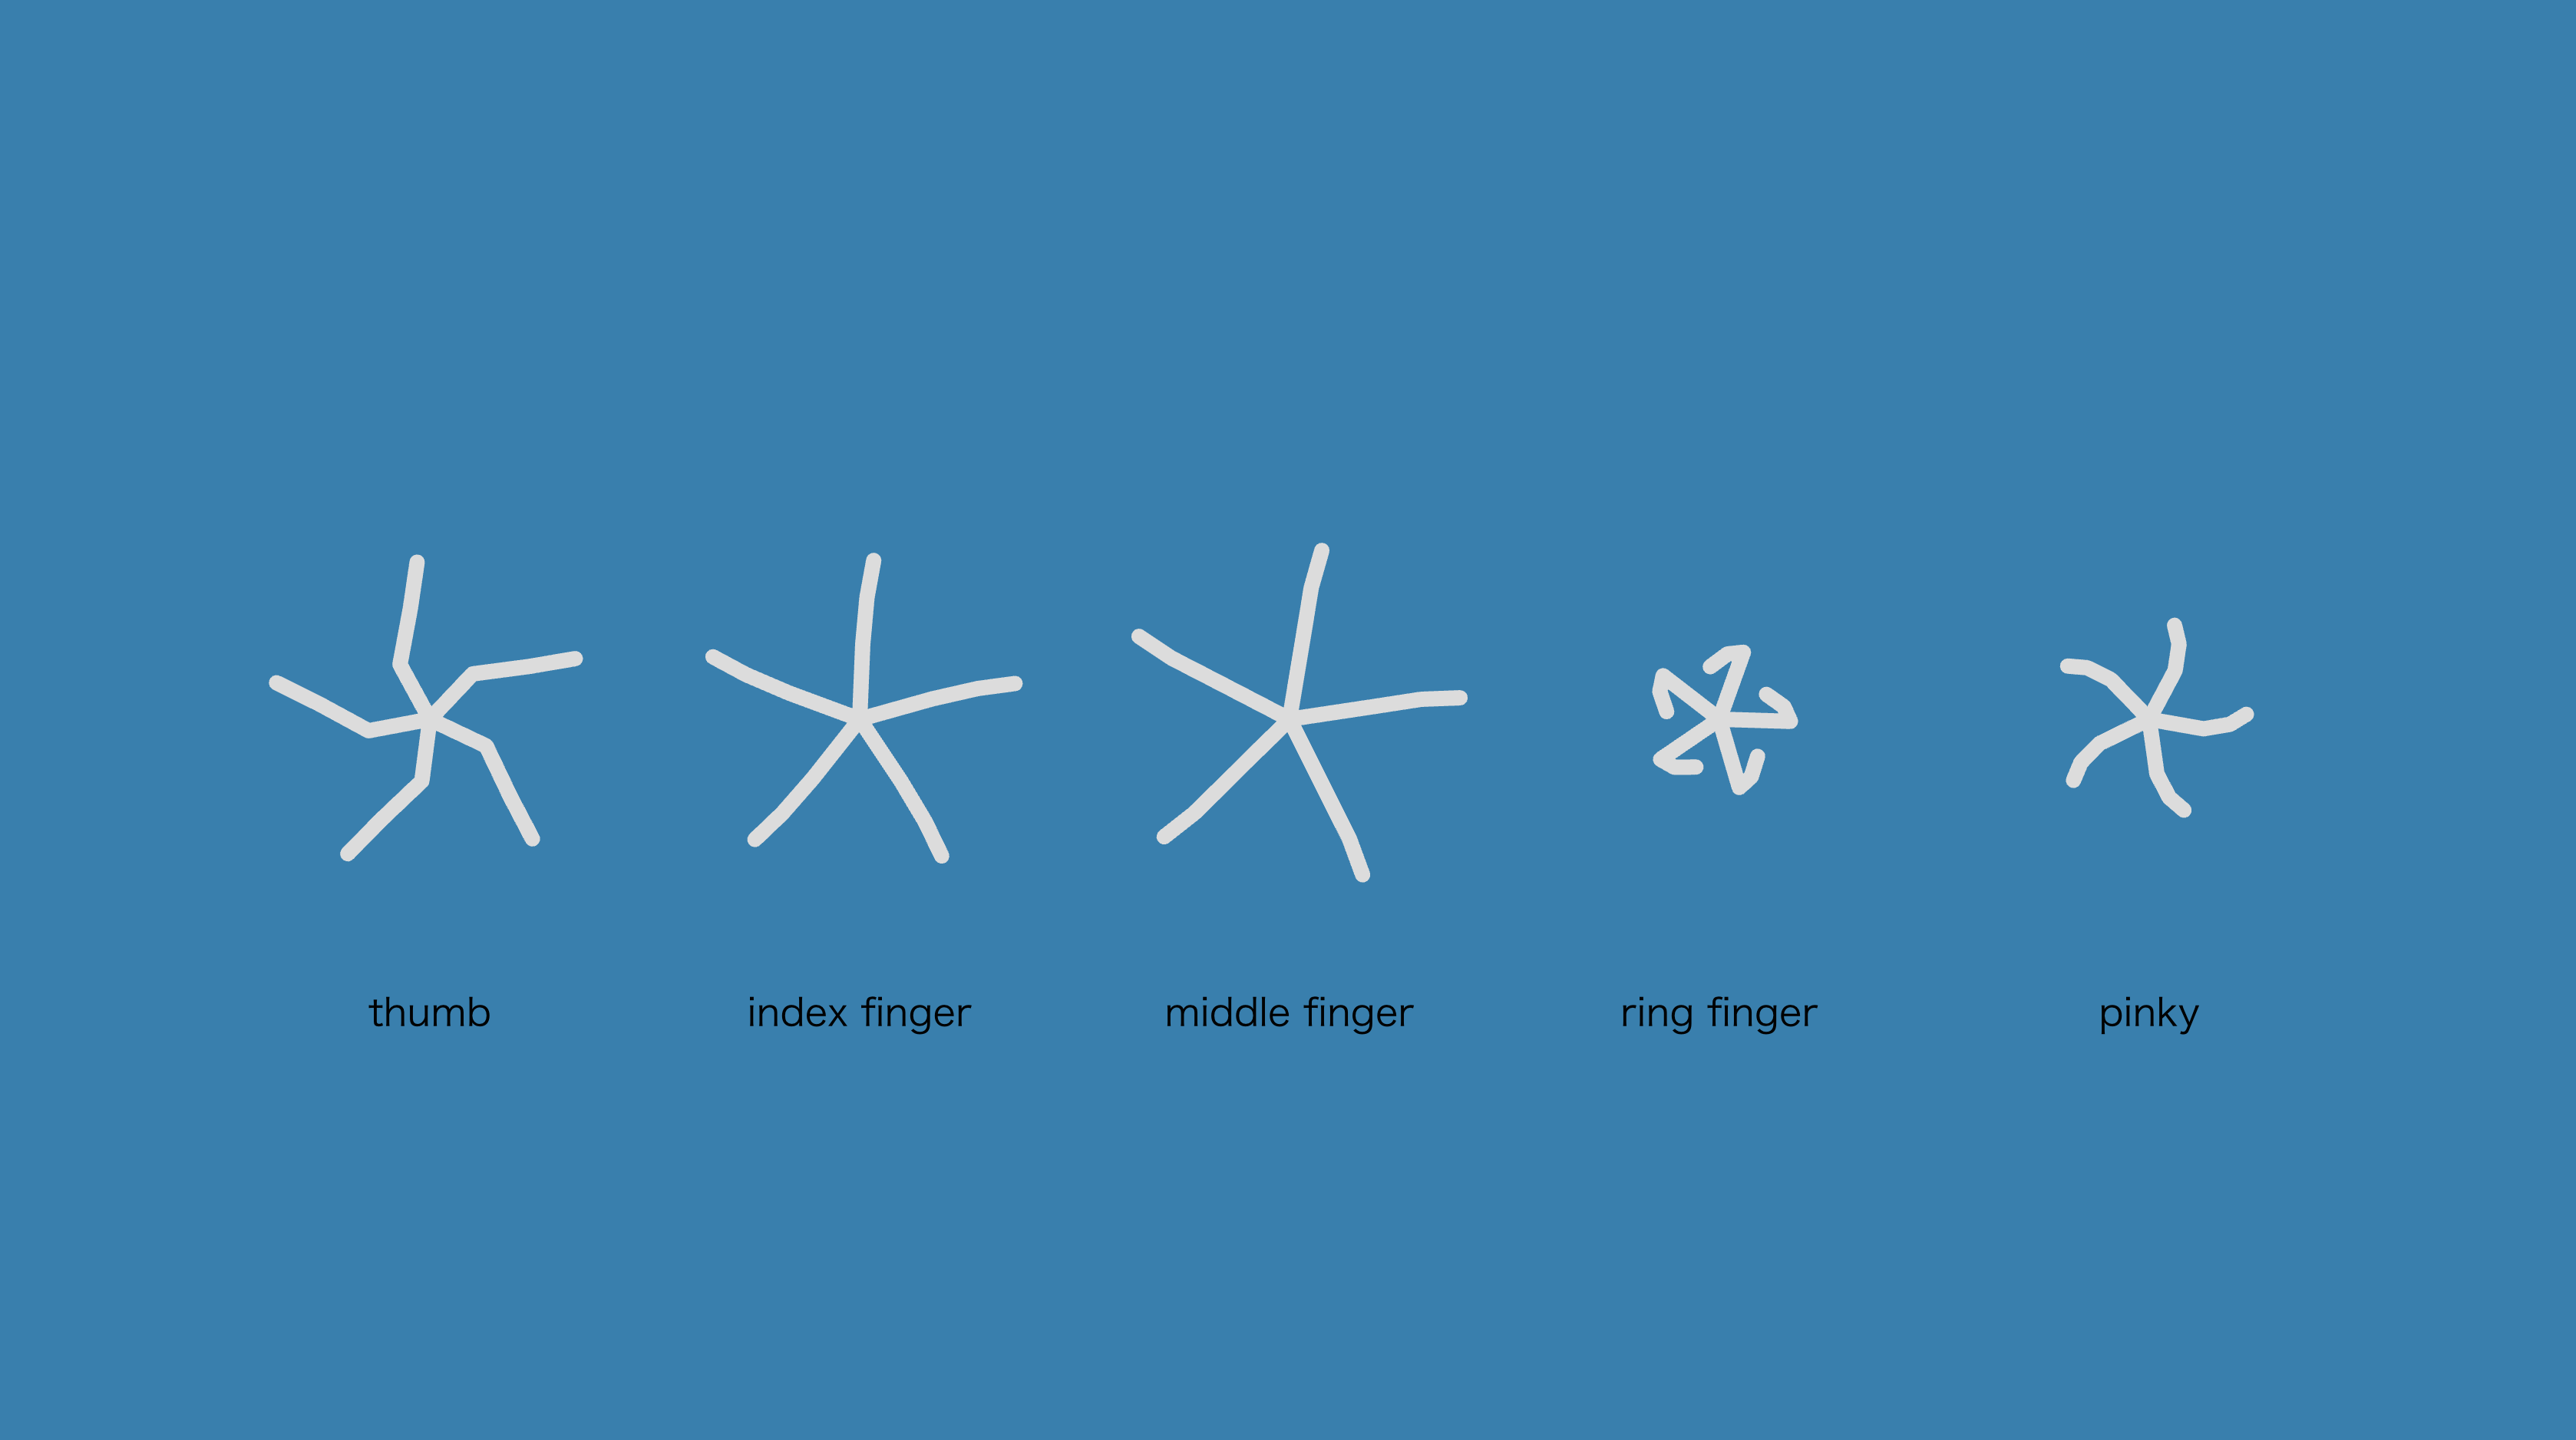
\includegraphics[width=15cm]{img/openhouse2022_interface.png}
  \caption{Digitizeのインターフェース(2022年)}
  \label{fig:exhibit_2022_interface}
\end{figure}

しかし展示を行うと、この習作の当初想定していなかった魅力に気づいた。それは、指の動きが単に、別の構造にマッピングされただけであるのに、別の構造の手を動かす体験はそれだけで興味を惹くものだということである。手指の異なる形状への変換が3パターン展示された状態のこの展示で、10分以上興味を持って体験する方が複数名いた。そして、仕組みとしては指先と付け根の距離をとっているのだが、その変換処理を「正しく」理解していなくても、異なる方法で理解しているように思われる人が何人かいた。指先と付け根の距離を評価して変換していても、カメラに対して手を近づけたり遠ざけたり、手首から傾けたりすることでも動かすことはできる。そのためか、さまざまな「わかり方」があったのだと考えた。仕組みを知っている制作者にとっては自明なことだが、自己の運動とどう対応するのかを知り得ない体験者は、自身の体を動かして観察されたことを通して推測することになる。それゆえに、この仕組みを通して思い描く身体像に、体験者ごとに違いがあるのではないか。

こうした体験者ごとの違いは、「わかりやすい」ものを対象としたときよりも、「わかりにくい」ものを対象としたときの方が顕著に現れると考えた。その上で、わかったようで分からない、行きつ戻りつな感覚に陥りながらも、飽きずにそれを分かろうとして向き合う様子が続いたことに、先の問題意識に応えるものがあるのではないかと考えた。

\section{本研究の目的}

本研究の目的は、人と道具、機械、あるいは人体の中にある他者性との関係における「人馬一体」のような一体感について捉えることである。そして、そうした関係性はどのようにして引き出すことができるのかを提示することである。

\section{本論文の構成}
(提出前に、全文章を概観した上で書き直す)

本章では、研究背景を問題提起の形で示し、研究の概要を示した。本研究が着目した「手指の異なる形状への変換」について、その観点から取り組む動機と、

第\ref{related_works}章では、「身体化」に関する先行研究について、それぞれの分野でどのように展開しているのかについてを概観する。そして、その中での本研究の位置付けと貢献を示す。

第\ref{prototyping}章では、手指の変換表現についての探索と、「人馬一体感」の生起に向けた意識的な試行が生じる体験として作品を構成するにあたっての取捨選択のプロセスを説明し、最終的な作品における構成の根拠を示す。

第\ref{about_grasper}章では、作品概要と、そこに至るまでのプロトタイピングの分析を通して、作品形態について説明する。

第\ref{validation}章では、そのようなねらいのもと制作された本作品が、実際どのように経験されるのかについての質的調査を行うため、Video Cued Recallという手法を用いて体験について振り返り、実際の体験がどのようなものであったのかを踏まえて、モデルとの関係性について考察する。

第\ref{考察}章では、行った調査の結果からどのような体験の作品であったかを振り返り、本作品が狙いとしていたこと、あるいはその範疇を超えて、作品として何が達成されたのかについて考察する。

第\ref{matome}章では、これまでの議論をまとめ、最後に今後の展望として、ここで制作を行ったモデルがそれ以外の議論とどのように関係し、今後どのような可能性を有するのかについて述べる。
\newpage

%----------------------------------------------------------------------
% 2章 関連研究
%----------------------------------------------------------------------
\chapter{関連研究}
\label{related_works}

\section{``身体化''としてのembodiment}
「身体化(embodiment)」は心理学や認知科学の領域で、「身体化感覚(sense of embodiment)」を中心として実証的知見が蓄積されている。身体化感覚は、身体に対する所有感(sense of body ownership)、行為主体感(sense of agency)、そして自己位置感覚(sense of self-location)を合わせた感覚として取り扱われることが多い\cite{kilteni2012}。その元となったのは、Gallagherの「ミニマルセルフ」という概念である。「ミニマルセルフ」とは、自我としてみなしうる必要最小限のもののことであり、身体所有感(sense of ownership)、行為主体感(sense of agency)の二つから構成されていると説明される\cite{Gallagher2000}。こうした自己についての説明を実験的に操作・検証可能であることを示したのがBotvinick \& Cohenによるラバーハンド錯覚\cite{BotvinickCohen1998}である。これは、自分の手を衝立の裏に隠し、ラバー製の手を目の前に置いた状態で、両方に同じタイミングで刺激を提示すると、偽物の手を自分の手であるように感じる錯覚である。この報告により、外界の対象への身体所有感の生起が可能であることが示されたとともに、身体所有感研究に関する系統的な手法が探求されることとなった。

VRやロボティクスにおいては、「私たちはどこまでを自分の身体として認識しうるか?」、すなわち「何を``身体化''できるのか?」について、その可能性と限界を探る研究や、そうした知見の応用を提唱する研究へと繋がっている。以下では、身体化感覚を中心に、これまでにどのような探求がなされており、またどういったことがわかっているのかについて、一例を紹介する。

VRを用いた身体化感覚の研究では、身体の別の部位への動きのマッピングや同時に操作する身体の数などを操作することで、新しい心理学研究の可能性を拓くような研究がなされている。例えば近藤ら\cite{Kondo2020}は、右手の親指の動きにVR上の左腕の動きを連動させることで錯覚的な身体所有感(Illusory Ownership)が生じるのかについて検証した。被験者は、右手の親指の動きがVR上での左腕の動きにマッピングされている様子をヘッドマウントディスプレイを介して確認する。実験では、被験者に5分間自由に指先を動かしてもらった後、VR上で左腕のあたりにナイフが突然出現する。このときの皮膚コンダクタンス反応(Skin Conductance Response, SCR)の計測と、身体化感覚(embodiment)に関するアンケートを20人の被験者に行った結果、この手法を通して右手の親指と左腕の結びつき(re-association)は、程度は弱いが誘発できると報告している。また佐々木ら\cite{sasaki2022multisoma}は、VR上で最大4つの身体を制御できるシステムを実装し、複数の身体を制御する際、人間の身体認知がいかに更新されるかについて検討した。実験では3つのタスクを設定し、視線情報、タスクのパフォーマンス、身体化感覚(sense of embodiment)についての主観評価により、これらの身体の認知を評価した。結果、人間は複数の身体を同時に操作することで、それぞれの身体に対して身体所有感(sense of ownership)や運動主体感(sense of agency)を持つことができると報告している。

また、身体化感覚は時間によっても変化する。Kielibaら\cite{kieliba2021robotic}は、ロボットで拡張された親指が人間の運動能力を拡張させることができるかどうか、そしてそれが手の神経表現や機能にどのような影響を与えるのかを調査するため、The Third Thumbというロボットの親指を用いた研究を行った。この親指は、足のつま先で操作することができる。5人の参加者は、5日間にわたってThe Third Thumbを装着し、実験室での使用と日常生活での使用が求められた。通常は両手を使って行うタスクをこの親指を駆使して片手で行い、その器用さ(dexterity)や身体化感覚(sense of embodiment)などの度合いが評価された。トレーニングを経て、認知的負荷が増加した場合や視覚が遮断された場合でも、親指の運動制御、器用さ、そしてThe Third Thumbに対する身体化感覚(sense of embodiment)が向上したと報告している。

さらに、こうした考え方をユーザインターフェースのような、身近な道具との関係性について議論するために援用する例も見られる。インターフェース研究者の渡邊は、ユーザインターフェースにおける「透明性」を実現する上で「自己帰属感(sense of ownership)」に着目した\cite{Watanabe2017}。ここで「透明性」とは、道具の使用において、使っている最中にはその道具自体を意識せずに身体の一部になったかのようになり、目的に集中できるようにすることとされている。そして、道具の透明性は「自己帰属感」によってもたらされると考え、マウスカーソルを対象に、ユーザインターフェースにおける自己帰属感を検証する「ダミーカーソル実験」を行った\cite{Watanabe2013}。この実験ではスクリーン上に、マウスと連動して動く通常のカーソ
ルの他に色形状の同じの複数のダミーのカーソルをランダムに動くように同時に提示する。被験者は動きのみでしか自身のカーソルを判別することができない環境になる。そしてこの実験によって、人は動きのみであっても複数のダミーカーソルの中から自身のカーソルを発見できると報告されている。どれが自分のカーソルか判別できることから、人間はカーソルに対しても自己を見出しており、自己帰属感が生起していると主張している。
これを踏まえて、ユーザインターフェースにおける自己帰属感を生起するために、操作時の動作とグラフィックの追従性が重要となることを指摘した。

\section{``一体化''としてのembodiment}
ここまで概観したように、「身体化感覚」をキーワードとしてその可能性や限界を探る研究が発展してきたが、この意味でのembodimentは、「人間の一部として対象が帰属しているような状態」についてのみ言及するものである。しかし、これらの議論において明言されていないが、区別しておくものがあるのではないだろうか。例えば、上記の事例におけるKielibaらがthe third thumbを通して確認した「sense of embodiment」は、5日間という比較的長い実験期間と、トレーニングを通して「sense of embodiment」が生起することを報告している。その過程においては、単に「人間の一部として道具が帰属する」というだけではなく、人間が道具の要領について学習することを通して、いわば「人間が道具に帰属する」という逆向きの関係が現れているとも言えるのではないだろうか。

Embodimentは日本語で「身体化、具体化」などと訳されるが、動詞の「embody」についてCambridge Dictionaryで引くと、
\begin{quote}
  \begin{enumerate}
    \item \textit{to represent a quality or an idea exactly} (質や考えを的確に表すこと) 
    \item \textit{to include as part of something} ((何かを)何かの一部として取り込むこと)
  \end{enumerate}
\end{quote}
とある\cite{embody}。ここで指摘したいのは、2つ目の意味からembodimentの原義とは「何かを取り込んで、何かの一部とすること」であり、「人間の一部として対象が帰属しているような状態」のみを指すわけではないということだ。

このように「embodiment = 一体化」として捉えたとき、その立場から人と他者との関係を捉えていると考えられる研究もいくつかある。

\subsection{人馬一体感}
心理学研究者の大北らは、ヒトとウマという異種間の間に芽生える一体感である「人馬一体」感について、どのようなプロセスで「人馬一体」感は生じるのか、またその「人馬一体」感はどのような感覚なのかを明らかにする目的で、馬術経験者に対するインタビューから概念生成を行った\cite{ohkita2018}。結果、人がウマに対して「扶助」と呼ばれる非言語シグナルに対して、時間的に接近してウマが行動を変化させたときに、操作主体感といった自己の身体保持感(sense of ownership)の拡張が生じるだけでなく、ウマというヒト(自己)以外のエージェントが協働したことによって「ウマと心が通じ合えた」といった円滑なインタラクション感も得ている可能性が示されたと報告している。このように、自己と他者との関係について、一方的に人に帰属するような他者の観点のみならず、ヒトとウマの間に芽生えた相互学習や、ヒトが対象に対して帰属していくような感覚を通して、一体感が生起することを捉える視点も存在する。

\subsection{Sydney Felsによるembodiment}
こうした一体化のプロセスを捉えるための分類を提案したのが、コンピューター工学者のSydney Felsである。Felsは2000年の論文、「Intimacy and Embodiment: Implications for Art and Technology」\cite{Fels}において、人間と対象との関係性を「embodiment」の観点から4つのカテゴリに分類した。
それぞれの説明は以下の通りである(括弧内は筆者訳)。

\textbf{\textit{Response}(応答):}\\
対象に働きかけ、その応答次第で何をするか決める、といった「会話」をするときの人と相手の関係に近い状態を指す。この時は、人と対象とのあいだに一体感は芽生えていない。Felsは、人と対象がこの関係下にあるときに感じる喜びとは、人が期待していたことに対して予想通りの反応が得られるかどうかにかかっているという。Felsはこの関係下にある状態の例として「コンピュータとそれに初めて触れた人」を挙げ、「なんらかの操作を通して得られた、便利な機能に喜んでいる状態、また逆に「有用な結果を得られず落胆する状態」と説明する。

\textbf{\textit{Control}(制御):}\\
人が対象を自分自身の延長と感じ、それを通して遊ぶことができている
その操作によって感情的な満足や美的体験を得る状態を指す。例えばピアノの演奏において、「音が出ている」ということだけでなく、自分自身の表現したいことが、不自由なくピアノを通して体現されていると感じるときの、一体感によってもたらされる心地よさがこれに該当する \footnote{「Control」においてFelsは、「自分自身の延長」として経験される感覚であり、またそれが追従性の高いグラフィックによってもたらされると説明する。これは、渡邊がマウスカーソルやスマートフォンに対して用いた「操作時の指とグラフィックの追従性が高い」インターフェースという説明と同等のものであると考えられる。このことからFelsの分類におけるControlは、渡邊の「自己帰属感」と重なる。}。

\textbf{\textit{Contemplation}(鑑賞):}\\
人が対象に対して働きかけることはないが、人がその対象からの信号やメッセージを内省や反映を通じて、感情的になったり美的体験を得る状態を指す。Felsはその具体例として、絵画の鑑賞体験を挙げる。

\textbf{\textit{Belonging}(帰属):}\\
対象によって人が動かされているような経験を指す。人はその対象によって提供される体験を通じて感情的な反応を得る。ここでは、対象が人の体験や感情を形作る役割を果たす。

\begin{figure}[H]
  \centering
  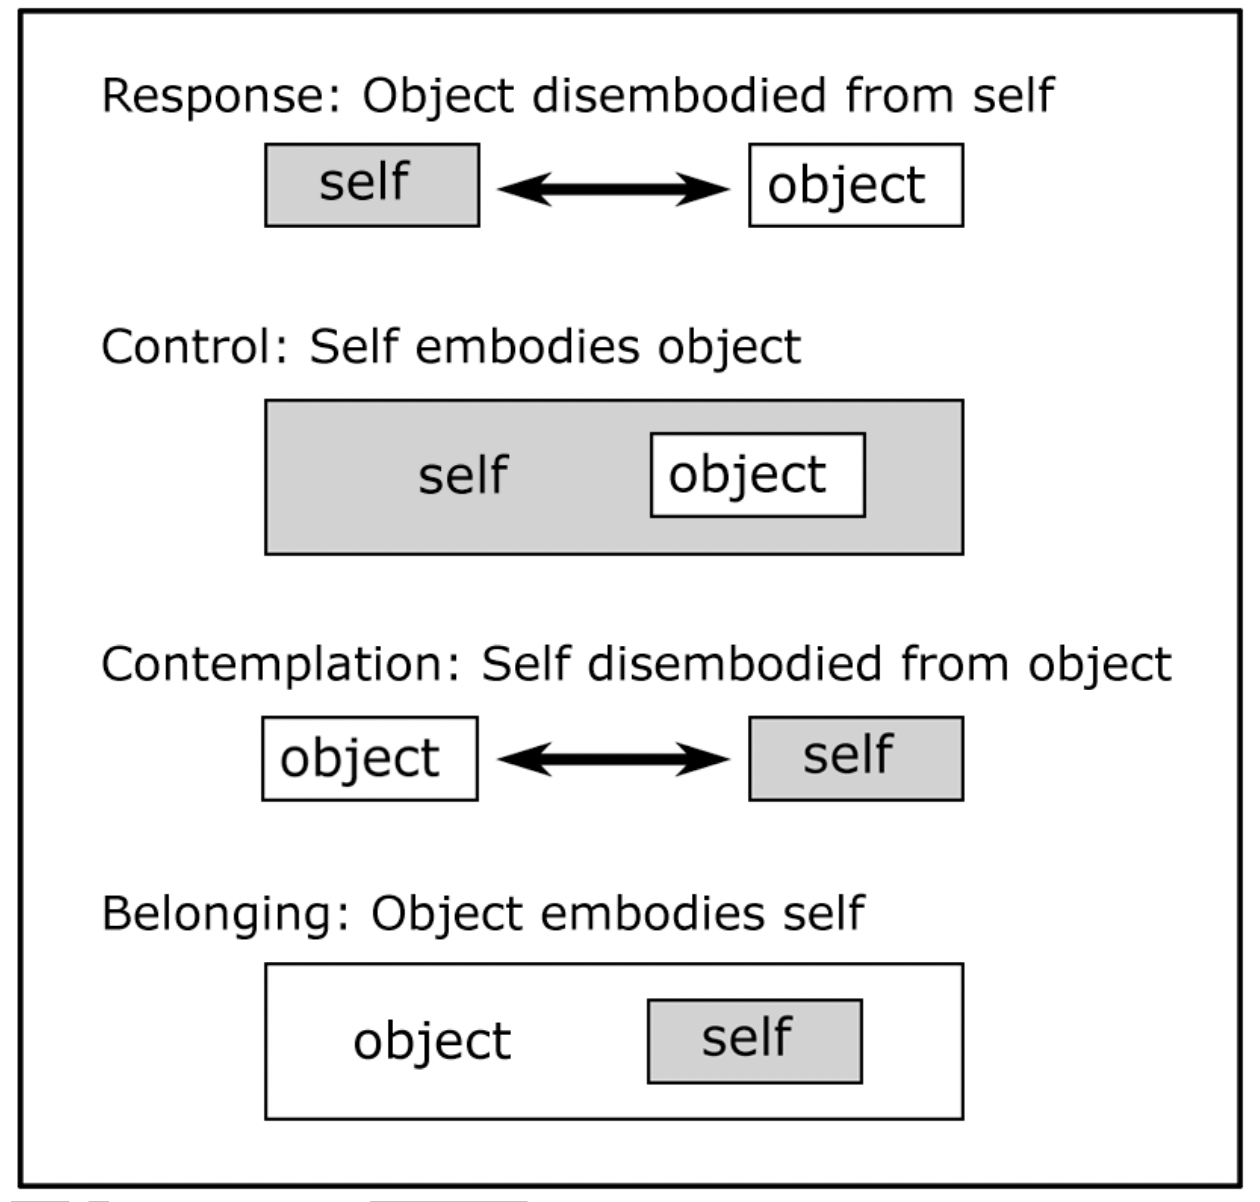
\includegraphics[width=8cm]{img/fels_diagram.png}
  \caption{Felsによるembodiment: Costelloらの論文より引用}
  \label{fig:fels_embodiment}
\end{figure}

% さて、Felsは特に、上記「制御 Control」においては「自分自身の延長」として経験される感覚について言及しており、またそれが追従性の高いグラフィックによってもたらされるという記述は、渡邊がマウスカーソルやスマートフォンに対して用いた「操作時の指とグラフィックの追従性が高い」インターフェースという説明と同等のものである。このことからFelsのいうControlとは、Gallagherの「sense of ownership」と同じものを指していると考えられる。その上で、embodimentの状態をControlのみならずBelongingから捉えていること、そしてembodimentが生じていない状態についても言及していることなど、現在HCIの分野で一般に用いられる意味でのembodimentよりも広く、人と対象を捉えるモデルとなっていることが確認できる。

% Felsの\textit{contemplation}や\textit{belonging}といった関係性は、他者と向き合い、一体化していくプロセスを捉える上で重要な区分であると考えた。そこで本研究が目指す「人馬一体感」を、Felsの用語を用いると、
% \begin{quote}
% \textit{Control}と\textit{belonging}が両方生起することで生じる\textit{Intimacy}  
% \end{quote}
% と説明できる。

本研究では、こうした「``一体化''としてのembodiment」の立場から、「自己」と「他者」の双方向的な一体感が象徴的に現れる「人馬一体」という言葉に着目し、そうした関係性のデザインを目指す。ここでの「人馬一体」感とは、大北らによる「人馬一体」感とは用法が異なり、例えば楽器やバイクなどにもみられるように、実現しようと思う自身の目的意識に対して、「自己」と「他者」のあいだで折り合いをつけていくことで生じる一体化の感覚を指す。こうした一体化のプロセスを捉えるために、本研究ではSydney Felsのembodimentの分類を用いて、作品の体験について分析することとした。
% 若干異なる。大北らの捉える「人馬一体」感は、「操作対象がエージェンシーを持つがゆえのインタラクティブな相互学習の過程を経て至る」感覚として特徴づけられる。

「人馬一体」感を引き出すにあたっては、人が無意識的に対象とインタラクトするのではなく、何かに注意を向けて、意識的にインタラクションすることで初めて\textit{control}する感覚が生起することが重要になってくるのではないか。本研究では、こうした観点を判断の基準として「手指の変換表現」について取り組んだ。


% ここで「身体化の過程」に注目すると、結果としては同じ身体化であっても、そこには質的な違いが存在することがわかる。例えばラバーハンド錯覚とThe Third Thumbは、いずれも身体化感覚が生起している点では共通する。しかし、前者は受動的な触覚提示によっても身体化が生じているのに対し、後者の身体化は「器用さ(dexterity)」を途中で獲得することで身体化が生じる。その過程では「もどかしさ」や「楽しさ」を経験すると考えられる。つまり、身体化するまでの意識的な試行期間の有無という点において異なっている。

% アバターに対して様々な介入が可能なVR分野では、身体拡張における可能性や限界を探る上で格好のフィールドであると言え、佐々木らや近藤らによる研究は、身体化感覚を評価軸とした様々な身体操作を実現するための基盤技術の研究であると位置付けられる。

% 一方Kielibaら\cite{kieliba2021robotic}の研究は、拡張された身体部位との協調(human-hand cooporation)が芽生えるまでの5日間という比較的長い調査期間を設け、身体化感覚の変化に着目している点で特徴的である。


% \section{身体の変換や拡張の試み}
% 身体の変換や拡張といったテーマは、embodimentの理論を踏まえて近年様々な研究が行われている。
% % 高度化・複雑化する技術が高い表現力や能力を持っていたとしても、それを扱う人間の能力が追いつかない限り、有効活用することができない。この問題は、群ロボット制御のような人間の身体性を越えた技術、そして身体の変換や拡張に取り組む分野で顕著に現れる。

% % Kimらは、複数台の卓上ロボット群を効果的に制御するための、インタラクション様式のセットと、そのデザインガイドラインを提示した。複数台で連携を取り合いながら、柔軟に役割を変えて複雑なタスクを達成することのできる群ロボットには、個々のロボットが持つ能力の総和以上の可能性がある一方で、それらを効果的に操作するためのインタラクション様式の設計に関する研究は少ない。そこで、卓上ロボット群に達成してほしいタスクを伝えられた被験者が、実際に卓上ロボットを前にしたとき、どのような働きかけをしてそれらを動かそうとするのかを観察することで、自然なユーザの動きを引き出すという手法(Elicitation Study)によって、様々なシチュエーションに対する適当なインタラクション様式を示した。

% % 稲見らによる自在化身体プロジェクト\cite{jizai}では、人間がロボットや人工知能などと「人機一体」となり、自己主体感を保持したまま自在に行動することを支援する「自在化技術」の開発と、「自在化身体」がもたらす認知心理および神経機構の解析をテーマにウェアラブル技術やバーチャル環境における共有身体の操作における基盤技術の開発に取り組む。
% 近藤らは、右手の親指の動きにVR上の左腕の動きを連動させることで錯覚的な身体所有感(Illusory Ownership)が生じるのかについての検証を、20人の被験者を対象に行なった\cite{Kondo2020}。モーショントラッキングを用いて取得された右手の親指の動きがVR上での左腕の動きにマッピングされている様子を、被験者はヘッドマウントディスプレイを介して確認する。実験では、5分間自由に指先を動かしてもらった後、VR上で左腕のあたりにナイフが突然出現する。このときの皮膚電導反応(Skin Conductance Response, SCR)の計測と、一体化(embodiment)に関するアンケートの結果から、この手法で錯覚的な身体所有感は確実に誘発できるものの、その程度は弱いと報告している。

% また佐々木らは、VR上で最大4つの身体を制御できるシステムを実装し、複数の身体を制御する際、人間の身体認知がいかに更新されるかについて検討した。実験では3つのタスクを設定し、視線情報、タスクのパフォーマンス、主観評価により、これらの身体の認知を評価した。結果、人間は複数の身体を同時に操作することで、それぞれの身体に対して身体所有感(sense of ownership)や運動主体感(sense of agency)を持つことができることがわかった。\cite{sasaki2022multisoma}。

% これらの研究は、親指の動きで動く左肩や複数の身体など、自分の肉体とは異なる身体ではあるが、それを自分の身体であるかのように認知しやすいものとそうでないものとの境界を探っていくこと、ひいては人間の認知的特性の理解に関心があると捉えられる。

% 一方で、次に紹介するKielibaらの研究は、同じく身体性(embodiment)についての評価が含まれるが、変換された身体のもとで行動する期間が長く、時間を経て身体性が獲得されることについて取り組んでいる。

% % 身体の変換や拡張を行う研究は近年、数多く行われている \footnote{近年に多いとする根拠は、小鷹の「ラバーハンド錯覚の遅い発見問題」という問題意識に基づく。小鷹は、「ラバーハンド錯覚」というシンプルな錯覚が学術的にはじめて発表されたのが1998年と遅く、それが「コンピュータの普及により、事物を情報的に処理する感受性が世界に浸透しつつあった1990年代後半」であったことに、単なる偶然ではない「情報としての身体」という発想を後押しするものがあったのではないかと指摘する\cite{kodaka}。}\cite{Kondo2020, ekusute,Kasahara2017,augmented_hand_series}。そうした実践の中心的な関心について、ここでは「錯覚」と「身体に対する再注目」であるとして、先行事例を紹介する。その上で、それぞれの関心と本研究の関心の相違点を説明することで、研究の位置付けを明らかにする。

% % しかし本研究の関心は「錯覚」ではない。そうではなく、突然自分の体とは似ても似つかない、それでいて扱い方もわからないような身体を与えられたときに、どう一体化していくかということに関心がある。

% % 小川らによる「えくす手(Metamorphosis Hand)」\cite{ekusute}では、指の伸びた手などの現実の身体にはあり得ない特性を持ったバーチャルな身体を通じてピアノを演奏することができる。そのねらいは、「現実とは異なる特性のバーチャルハンドへの身体所有感の生起を通じ、現実の身体的制約を超えたインタラクションを実現する、一種のバーチャルな身体拡張体験を提供する」と説明される。

% 身体所有感の生起要因に関するこれまでの議論を参照し、本作は「テクスチャ、形状、空間的配置、解剖学的構造の4つの特性」を根拠に、身体所有感が生じながらも、自己身体と意味的に類似しないバーチャルハンドを制作している。これらの特性は、身体所有感を生じさせる上での実証的知見ではあるが、本研究が対象とするIntimacyは、例えば楽器のように、こうした生起要因を押さえなくとも、習得を経て生じうるのではないかと考える。また、生起要因を多く踏襲しているわけではないからこそ、身体所有感が生じるまでには期間を必要とし、その程度にも個人差が生じるのではないだろうか。これらの観点から、本研究の取り組みは「えくす手」よりも極端な身体変容を促す体験として位置付けられる。

% \subsection{身体に対する再注目}
% Golan Levinらによる《Augmented Hand Series》\cite{augmented_hand_series}は、ウェブカメラによって取得した体験者の手の映像をリアルタイムに変形し、指の本数や長さなどの異なる手を投影する作品である。また、佐藤雅彦らによる「君の身体を変換してみよ展」では、さまざまなアプローチで身体の変容を扱う作品が展示されたが、その中でも《点にんげん・線にんげん》\cite{sato_icc}という作品では、動物の関節などの位置を示す点の動きだけでも脳が「生物的な動き」としてひとまとめに認識できる(バイオロジカルモーション)という現象を活用し、体験者の関節の位置が表示された点群が、様々な方法で結びつけられたり、ある役割を与えられるなどの「変換」に対して、「自分の身体である」という認識が保たれたまま形が変わっていく作品である。

% これらの作品の関心は、「身体に対する再注目」であると考えた。いずれも、身体が異なる見た目に変わったというだけであって、実用的な特別な能力が付与されたり、ゲーム性があるわけではない。それでも身体を動かしてみることの動機は、「動くこと」そのものへの興味が働いているからである。これは、生後まもない乳児が自分の手の存在に気づき、手を見つめたり、動かしたりしながらよく観察する動作である「ハンドリガード」に似た現象であると解釈した。「身体の変換」を通して、新しい身体像を得たことから生じた「注目」と向き合う契機となる。

% こうした関心の作品を、ここでは生まれ持った肉体に対する「注目」を最初と数えて、「身体に対する再注目」とした。

\newpage

\chapter{プロトタイピング}
\label{prototyping}
本研究では、「手指の変換表現」についての\ref{prototyping_concept_making}節のような動機を起点に「人馬一体感」のデザインが目的となり、修士作品《Grasp(er)》を制作した。ここでは、その過程にあるプロトタイピングについて説明する。
本章ではまず、それらのプロトタイプについて、「形状」、「マッピング」、「時間操作」、「ボール操作」の観点から分類する。その上で、これらのプロトタイピングFelsの分類を用いて分析し、「人馬一体感」を具現化する表現となりうるものについて述べる。

\section{プロトタイプの分類}
修士作品の制作に至るまでに、2022年6月から2023年10月までの期間で、OOという目的で総計60パターンのバリエーション、並びに計6回のプロトタイプの展示を実施した。プロトタイピング、並びに修士作品には、Tensorflowの開発グループがサンプルとして提供するhand-pose-detection\footnote{\url{https://github.com/tensorflow/tfjs-models/tree/master/hand-pose-detection}}を用いた。このモデルでは、手指の動きが下図\ref{fig:keypoints}に示す21個のキーポイントで表現される。こうしたキーポイントの情報をもとに、その配置や関係性といった構造、そしてそれをどのように表現するのか、といった点から変換表現について検討した。先入観で判断しないよう、この段階では先の研究目的を意識せず、このような探索空間の中で思いつく限り実装することを重視してプロトタイピングをおこなった。

プロトタイピングは、形状、マッピング、時間操作、ボール操作などの観点から分類することができる。単に形を考えるだけでなく、どのようにマッピングさせるか、そしてどの時間の動きを用いるか等、さまざまな変換方法を検討した。本章ではこれらの分類に基づいて、制作したプロトタイプについて概観する。

\begin{figure}[H]
  \centering
  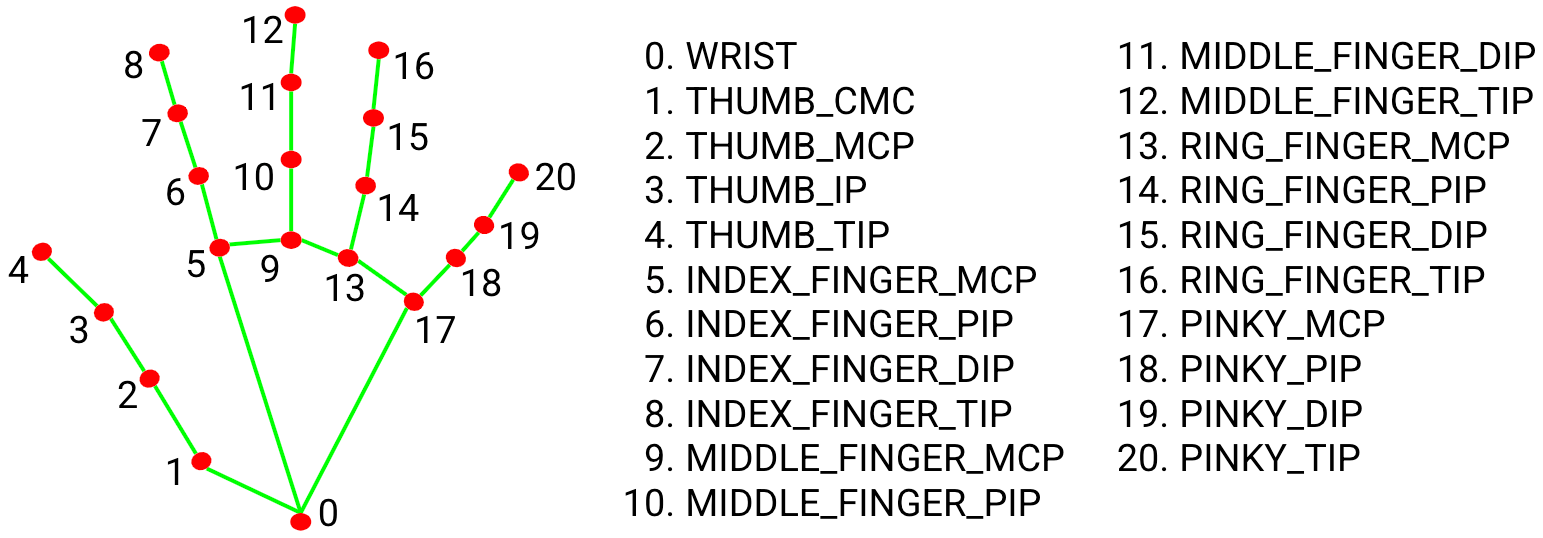
\includegraphics[width=15cm]{img/hand_keypoints.png}
  \caption{モデルを用いて表現されるキーポイント:hand-pose-detectionモデルのリポジトリより引用}
  \label{fig:keypoints}
\end{figure}

\subsection{形状}
形状については、指を1つのユニットとして捉えて、ユニット自体の形状やそれらをどのように関連づけるのかについて検討したもの、そうした枠組みとは無関係に制作したものとの2つに分類して説明する。
\subsection*{指をユニットと捉えたバリエーション}
キーポイントの情報を指ごとに分割して捉え、指一本の中で生じる動きを一つのユニットと捉えてバリエーションを展開した。以下の図\ref{fig:unit_valiation}に示す「ドット」や「ライン」は指のキーポイントを点群として離して出力するか、一つの線として繋げて表示するかの違いである。また、「円」、「くの字」、「クロス」などのバリエーションは、指先の\(y\)座標と指の付け根の\(y\)座標の差を評価して、ユニットの高さ(あるいは直径)が変化する。
\begin{figure}[H]
  \centering
  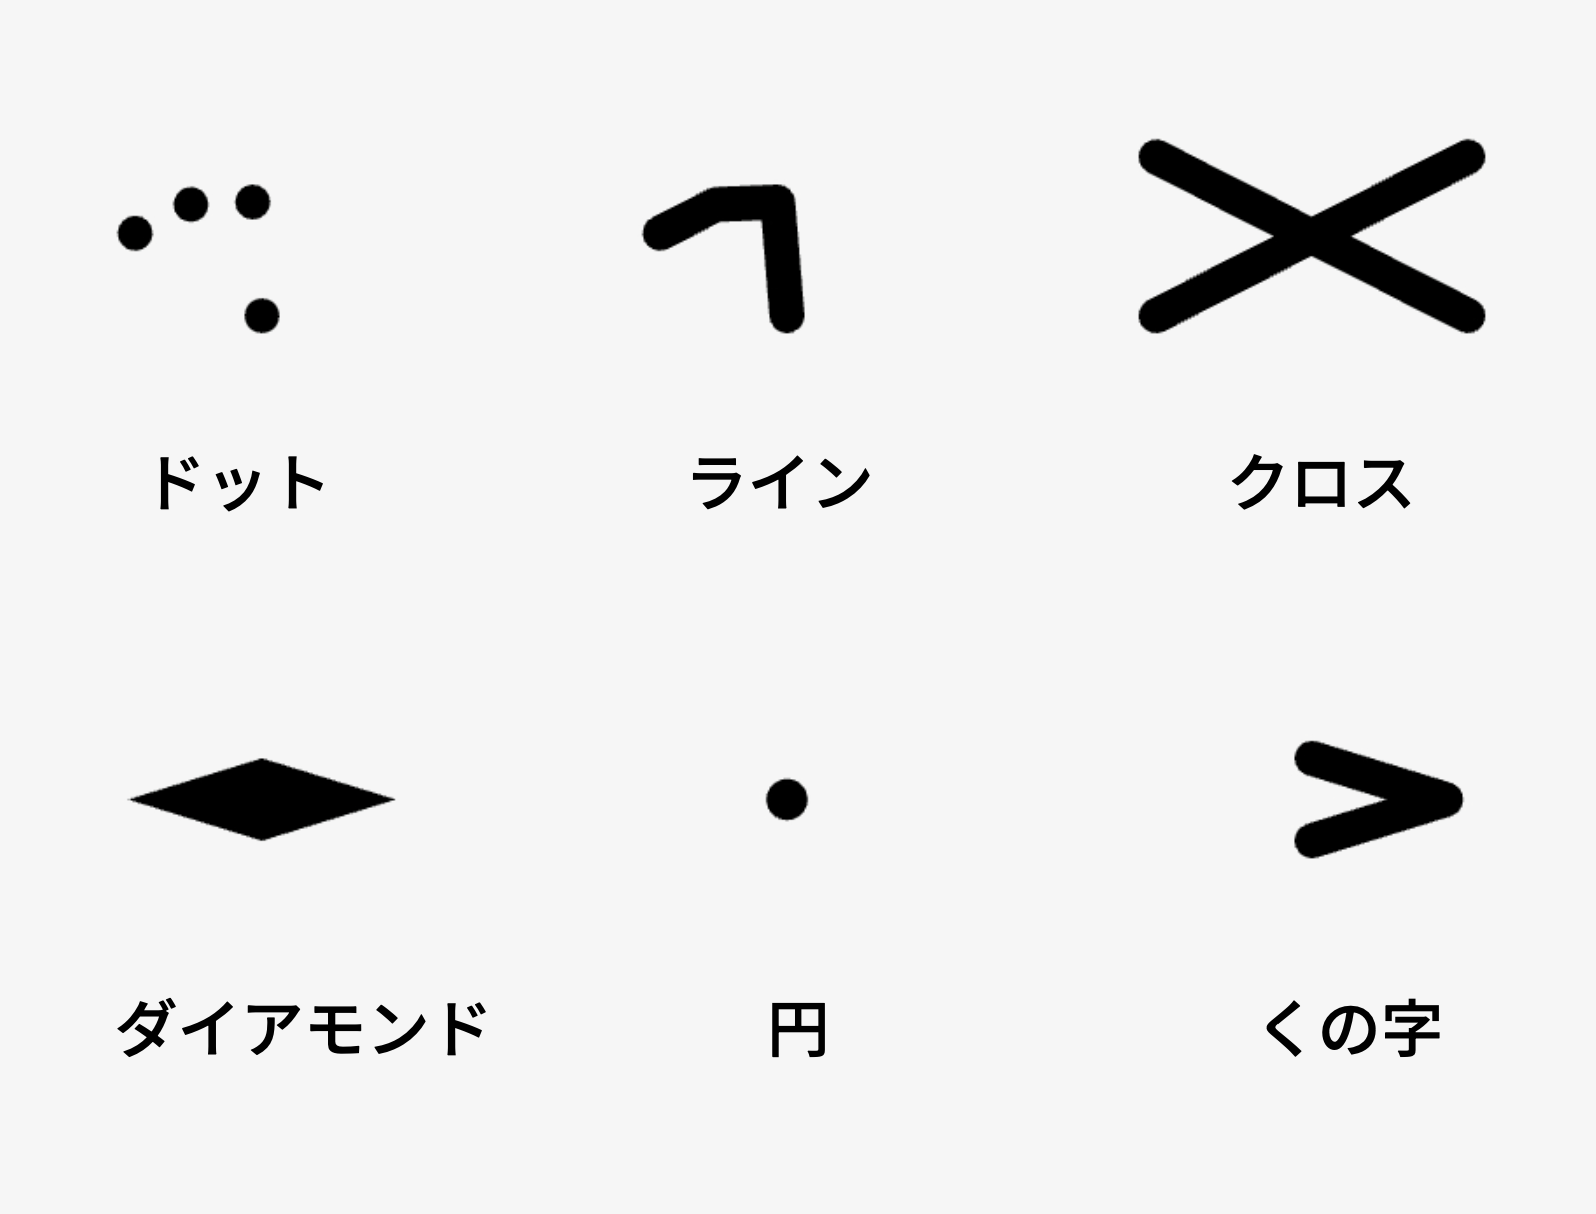
\includegraphics[width=10cm]{img/unit_valiation.png}
  \caption{ユニットのバリエーション}
  \label{fig:unit_valiation}
\end{figure}

また、これらユニットをいかに繋ぎ合わせて1つの形にするかについても探索を行なった(\ref{fig:connection_valiation})。以下は、同じ「くの字」のユニットについて、「並列に並べたもの」、「片手ずつ直列に繋ぎ、左右の同じ指の高さを結ぶ直線の傾きで回転をかけたもの」、「円形に繋げたもの」の3つのバリエーションである。(3枚画像を追加する)

\begin{figure}[H]
  \centering
  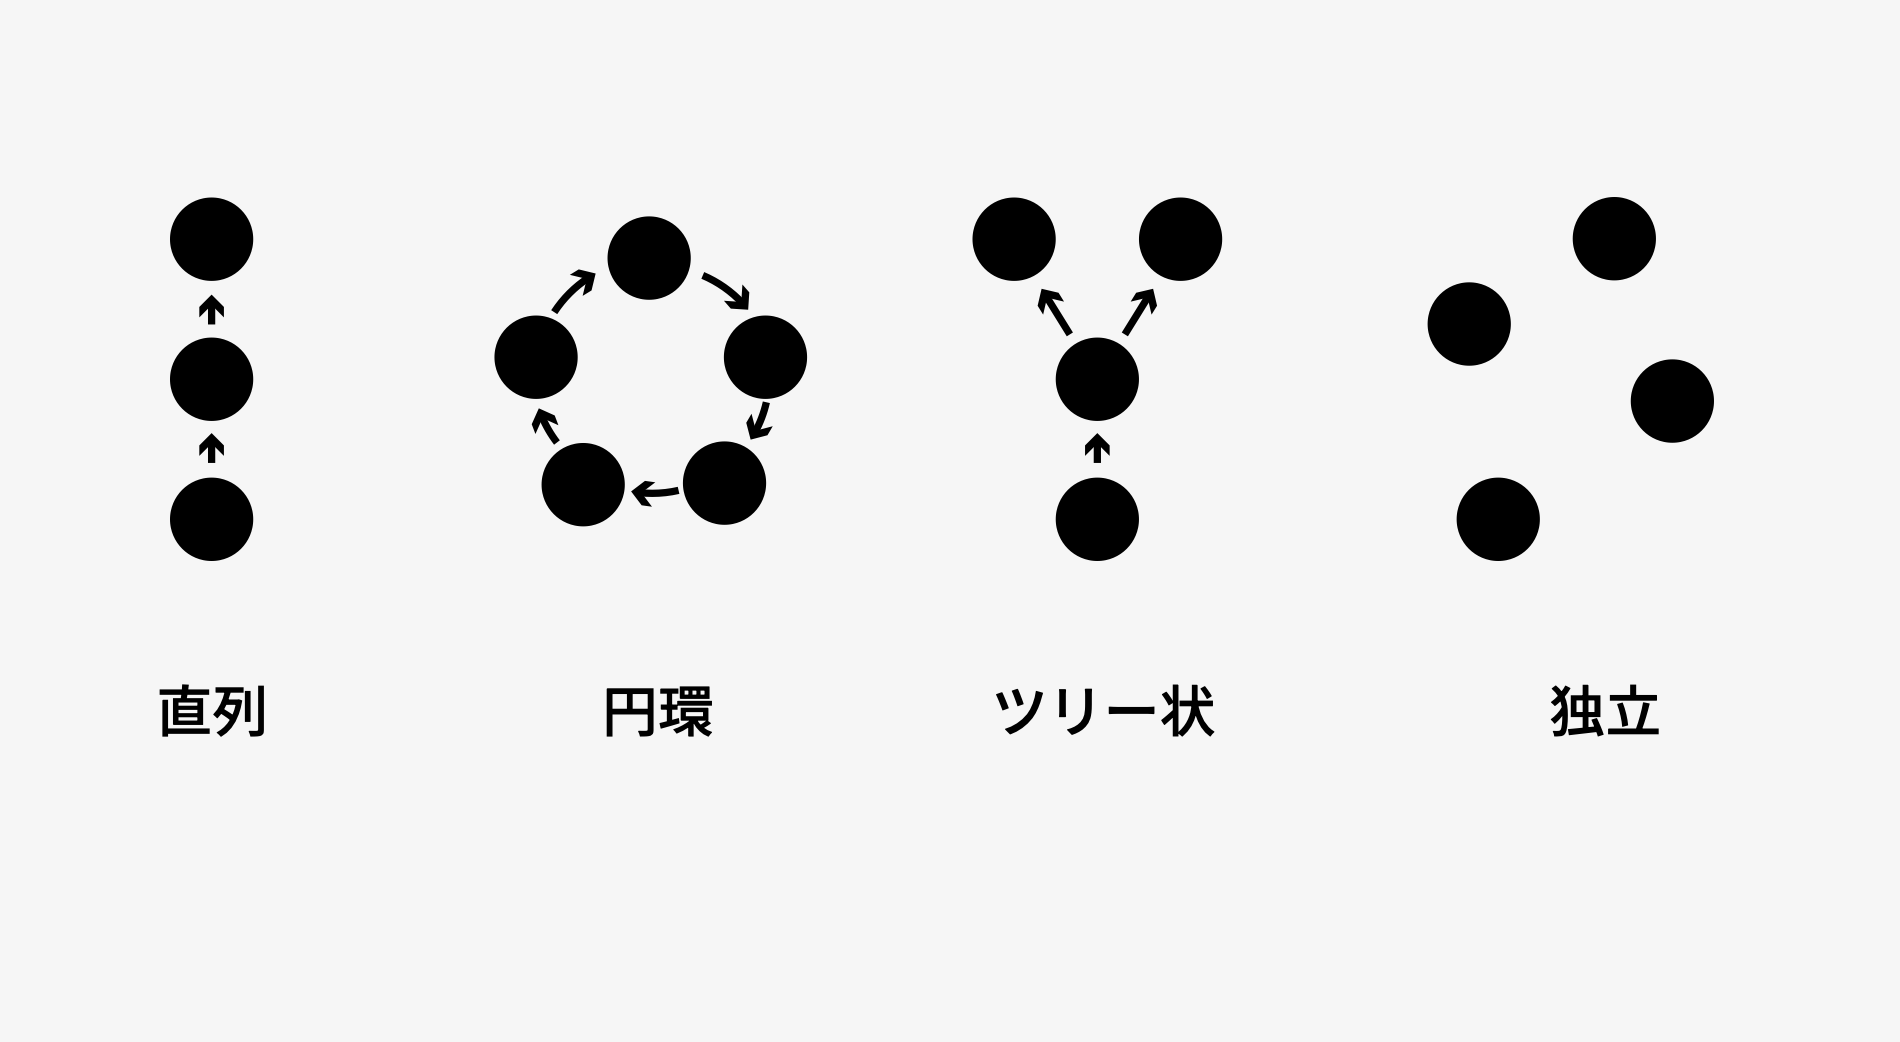
\includegraphics[width=10cm]{img/network.png}
  \caption{繋ぎ方のバリエーション}
  \label{fig:connection_valiation}
\end{figure}



\subsection*{指をユニットとしないバリエーション}
手指の動きを全て包み込む皮膜を「凸包(convex envelope)」のアルゴリズムを用いて実装したり、また指先と付け根の動きだけでなく、指の関節の開き具合を変数として、二等辺三角形の頂角の大きさが変化するバリエーションなどを作成した。

\subsection{マッピング}
マッピングについては、1つの動きが1箇所に対応しているものだけでなく、1つの動きを複数のパーツの動きへと複製したバリエーションなどを作成した。図\ref{fig:networked_finger}に示すプロトタイプ\footnote{\url{https://eee-handpose-playground.vercel.app/work/createNetworkedFingers}}では、指先をクリックすると5本ある指のうちのいずれかの動きを追従する指が、指先に追加されるものである。どの指が付け加わるかはランダムである。そのため指が新しく追加されるたびに、一本一本指を動かして、どこがその指に対応しているのかについて同定する必要がある。

またそのほかに、図\ref{fig:fractal_finger}に示すプロトタイプ\footnote{\url{https://eee-handpose-playground.vercel.app/work/fractalFingers}}は、フラクタル構造で指の動きを配置したバリエーションである。親指の先に人差し指の動きが複数分岐し、さらに人差し指の先から中指の動きが複数分岐して配置される。

\begin{figure}[htbp]
  \begin{minipage}[b]{0.5\linewidth}
    \centering
    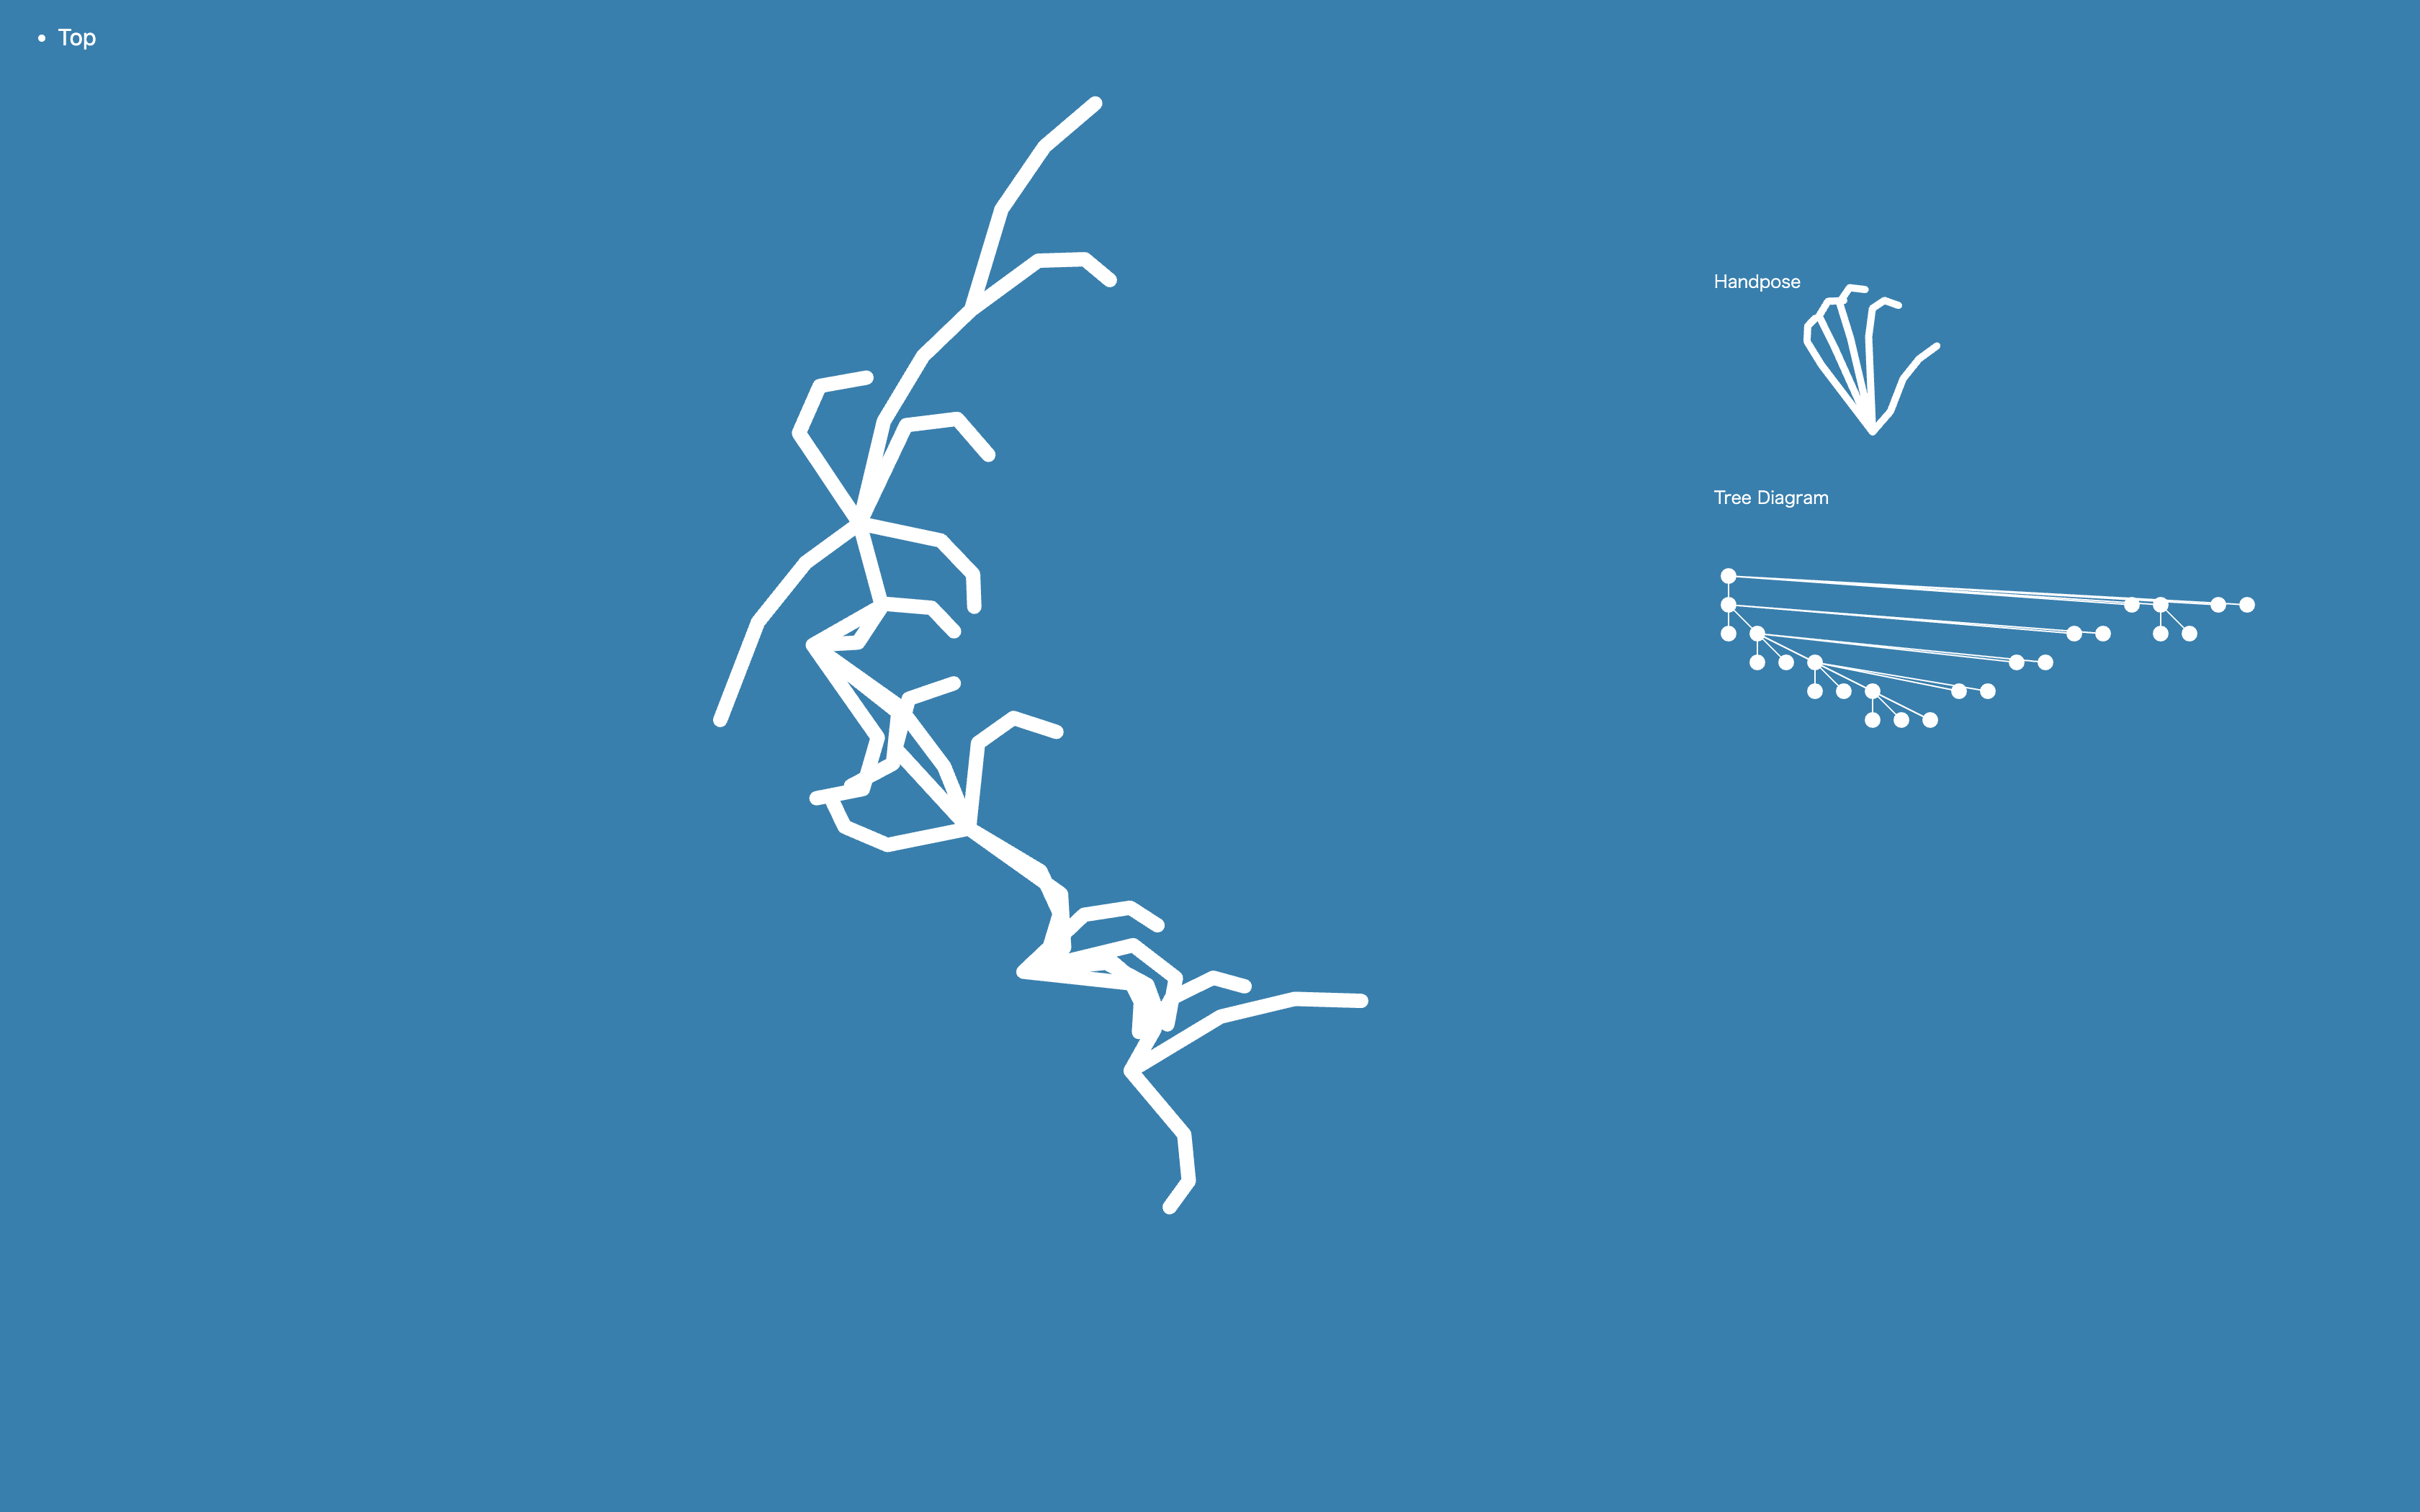
\includegraphics[keepaspectratio, width=7cm]{img/networked_finger.png}
    \caption{Networked Finger}
    \label{fig:networked_finger}
  \end{minipage}
  \begin{minipage}[b]{0.5\linewidth}
    \centering
    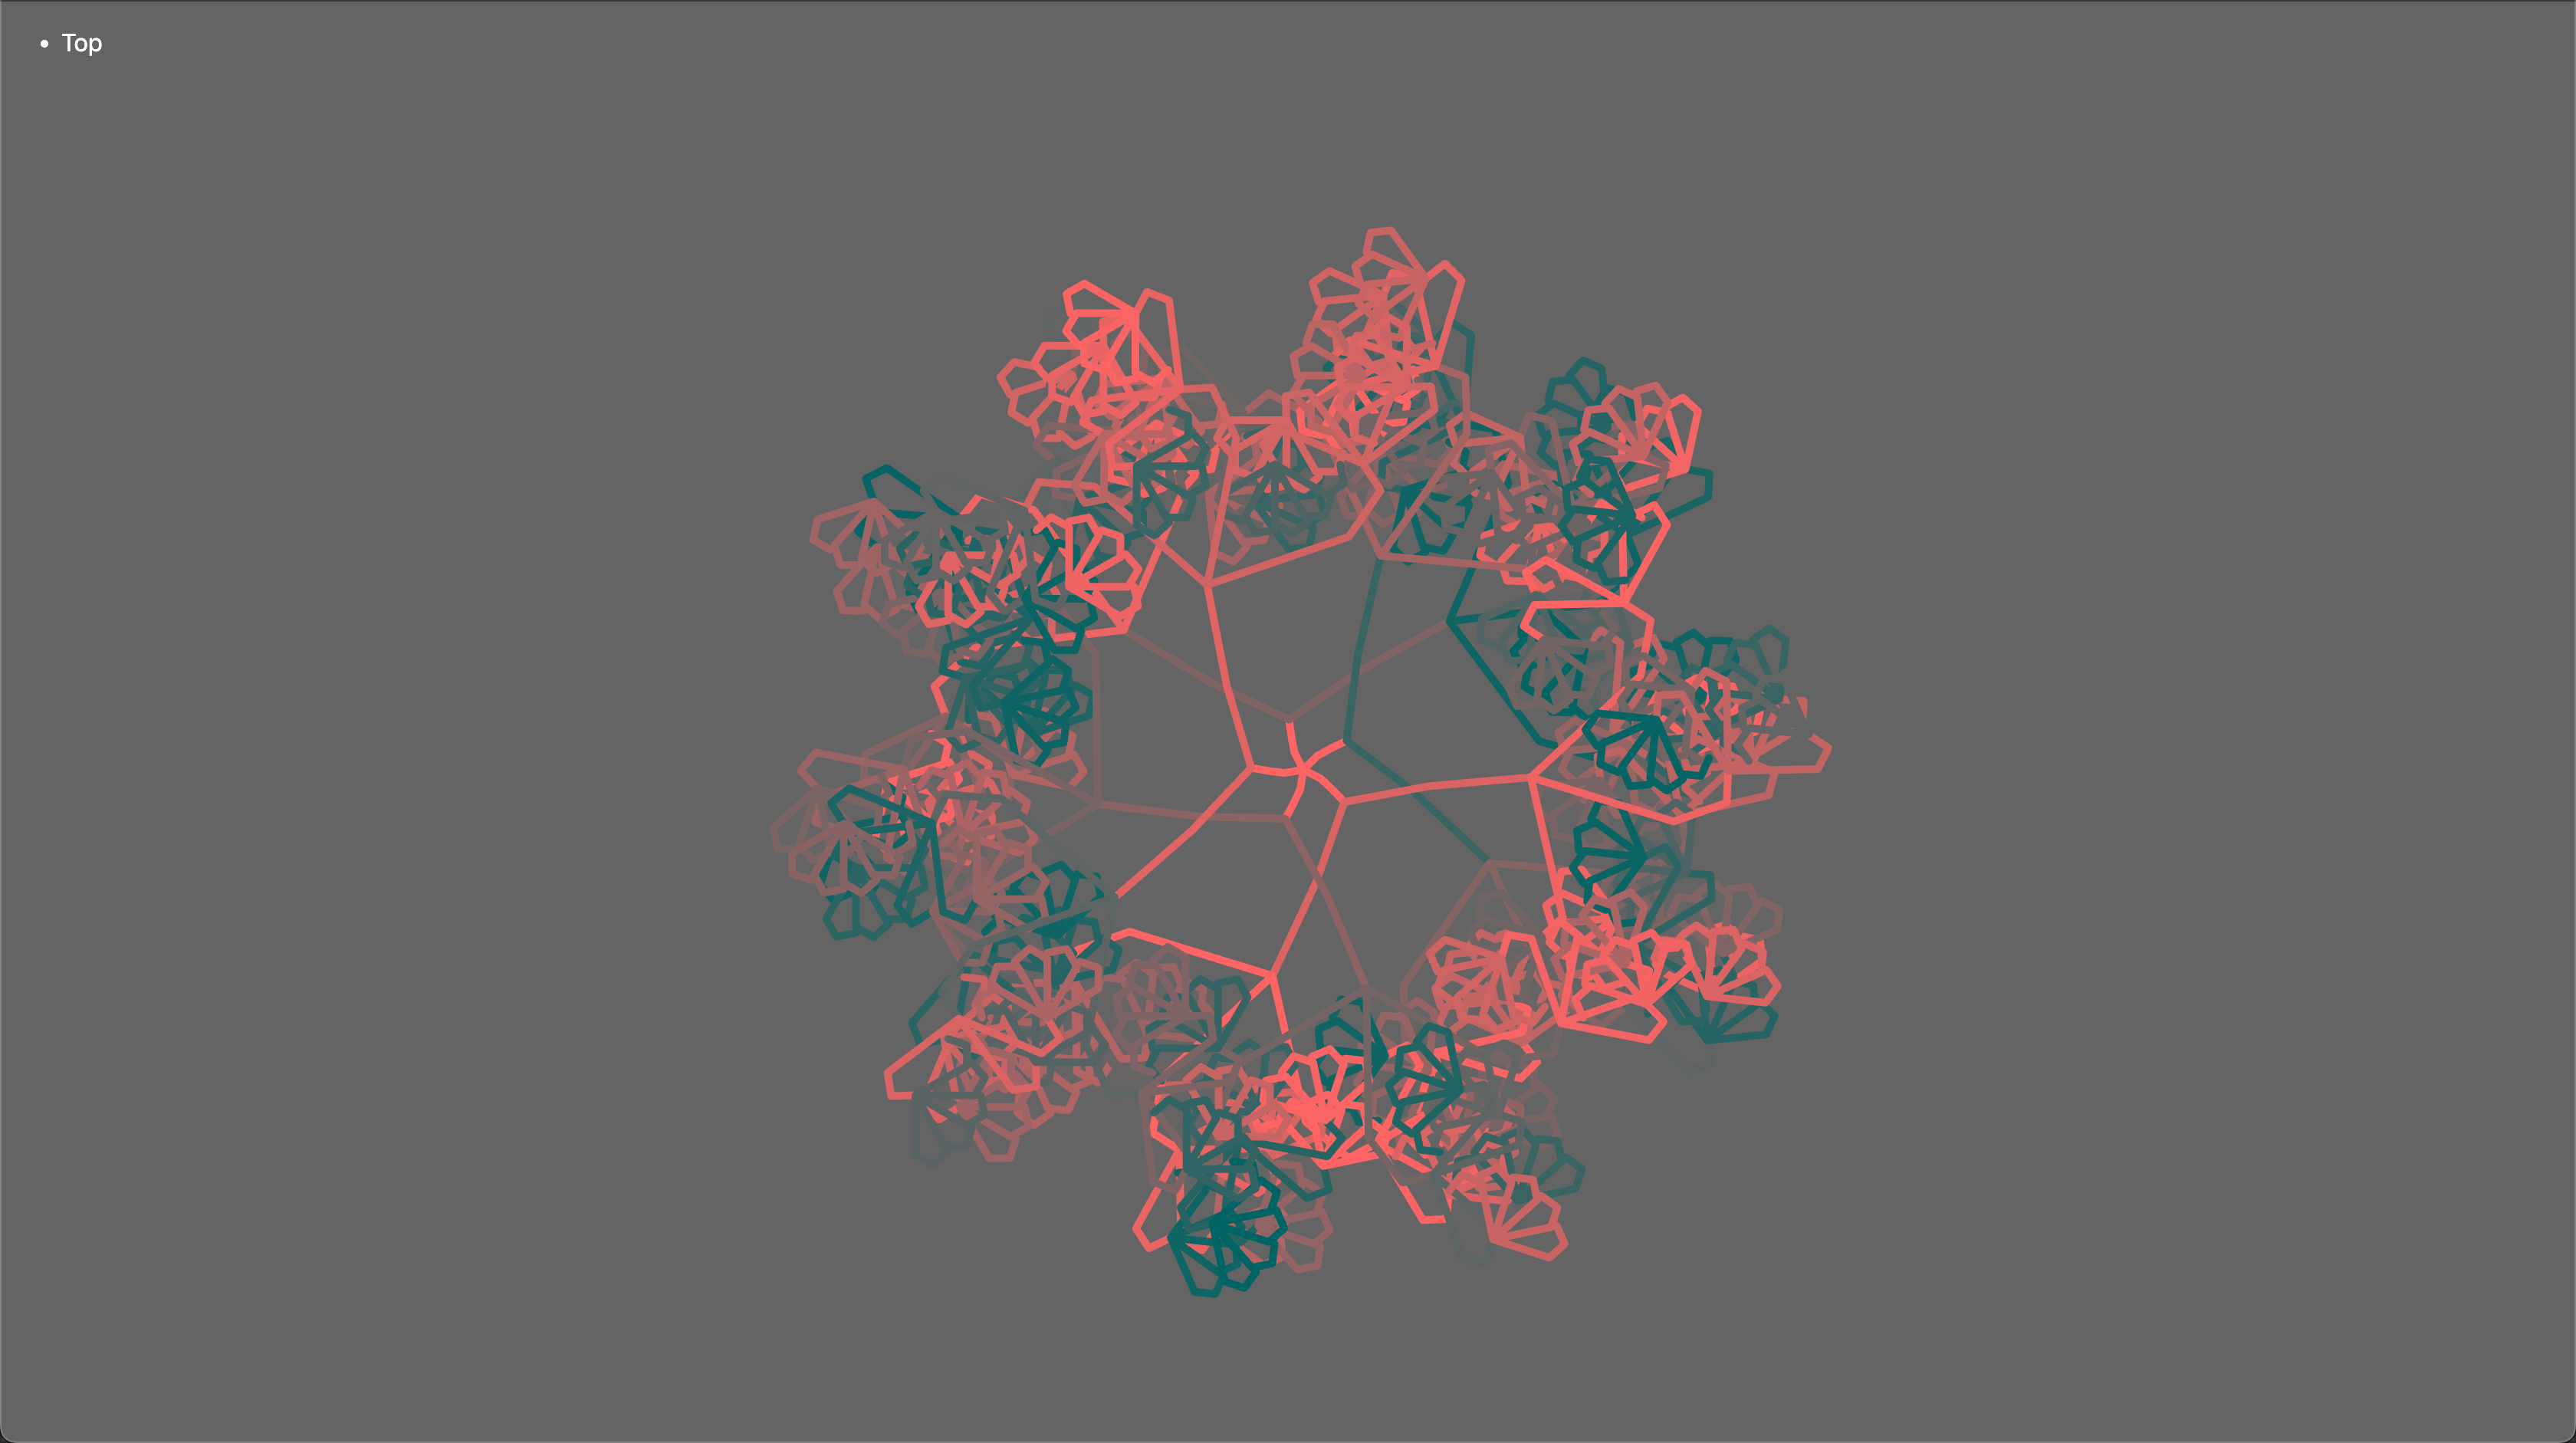
\includegraphics[keepaspectratio, width=7cm]{img/fractel_finger.png}
    \caption{Fractal Finger}
    \label{fig:fractal_finger}
  \end{minipage}
\end{figure}

\subsection{時間操作}
以下は、現在の自分の動きだけを表示するのではなく、過去の動きも表示するバリエーションである。図\ref{fig:prototype_delay}に示すプロトタイプでは、5本の指の動きが等間隔に並べられているが、それぞれの指は、鉛直上向きの角度に現在の指の動き、そこから時計回りに、順次過去の指の動きが並べられている\footnote{\url{https://interaction005-moe5dbh11-k1105.vercel.app/}}。このプロトタイプでは、指先を小さく動かすと、その動きが時計回りに伝播していくような動きが起こる。これは例えばゼリー状の物体を触れた時のような、物体の衝撃が全体へと伝播していくようすにも見立てられる。そのためか、柔らかいオブジェクトに触れているときのような手触りのようなものを感じた。
また、数ミリ秒前の動きが隣接する形に現れ、全体として2秒程の期間の全ての動きが表示されることになる。そのため、2秒間のあいだに動きの変化があれば、身体を動かしていても止まっていても画面に変化が現れることが、直感に反した動きとなることに注意が向く。

\begin{figure}[H]
  \centering
  
\includegraphics[width=15cm]{img/past_time.png}
  \caption{過去の動きを用いた例}
  \label{fig:prototype_delay}
\end{figure}

\subsection{ボール操作}
ここまでは手指をいかに変換するかについて探索を行なってきたが、その手指を用いた動きの複雑度に影響する要素としてボール操作について検討した。こうしたバリエーションを制作し、ボールがないものと並置して「IAMAS openhouse2023」にて展示した際、体験した方の一人から2つを比較して、手指の変換表現だけのものについては「途中から自分が何やってるか忘れてしまって、なんとなく指を動かすとなんとなく画面の描画内容が変わってる、となってしまっている」一方で「ボールの方はそんなことはなかった」とし、その理由として「具体的なタスクがあったほうがずっと続きやすい」といったことを挙げていた。そのため、よりタスクを明確化したバリエーションとして下記のような、マトあてのバリエーションも制作した。

\begin{figure}[H]
  \centering
  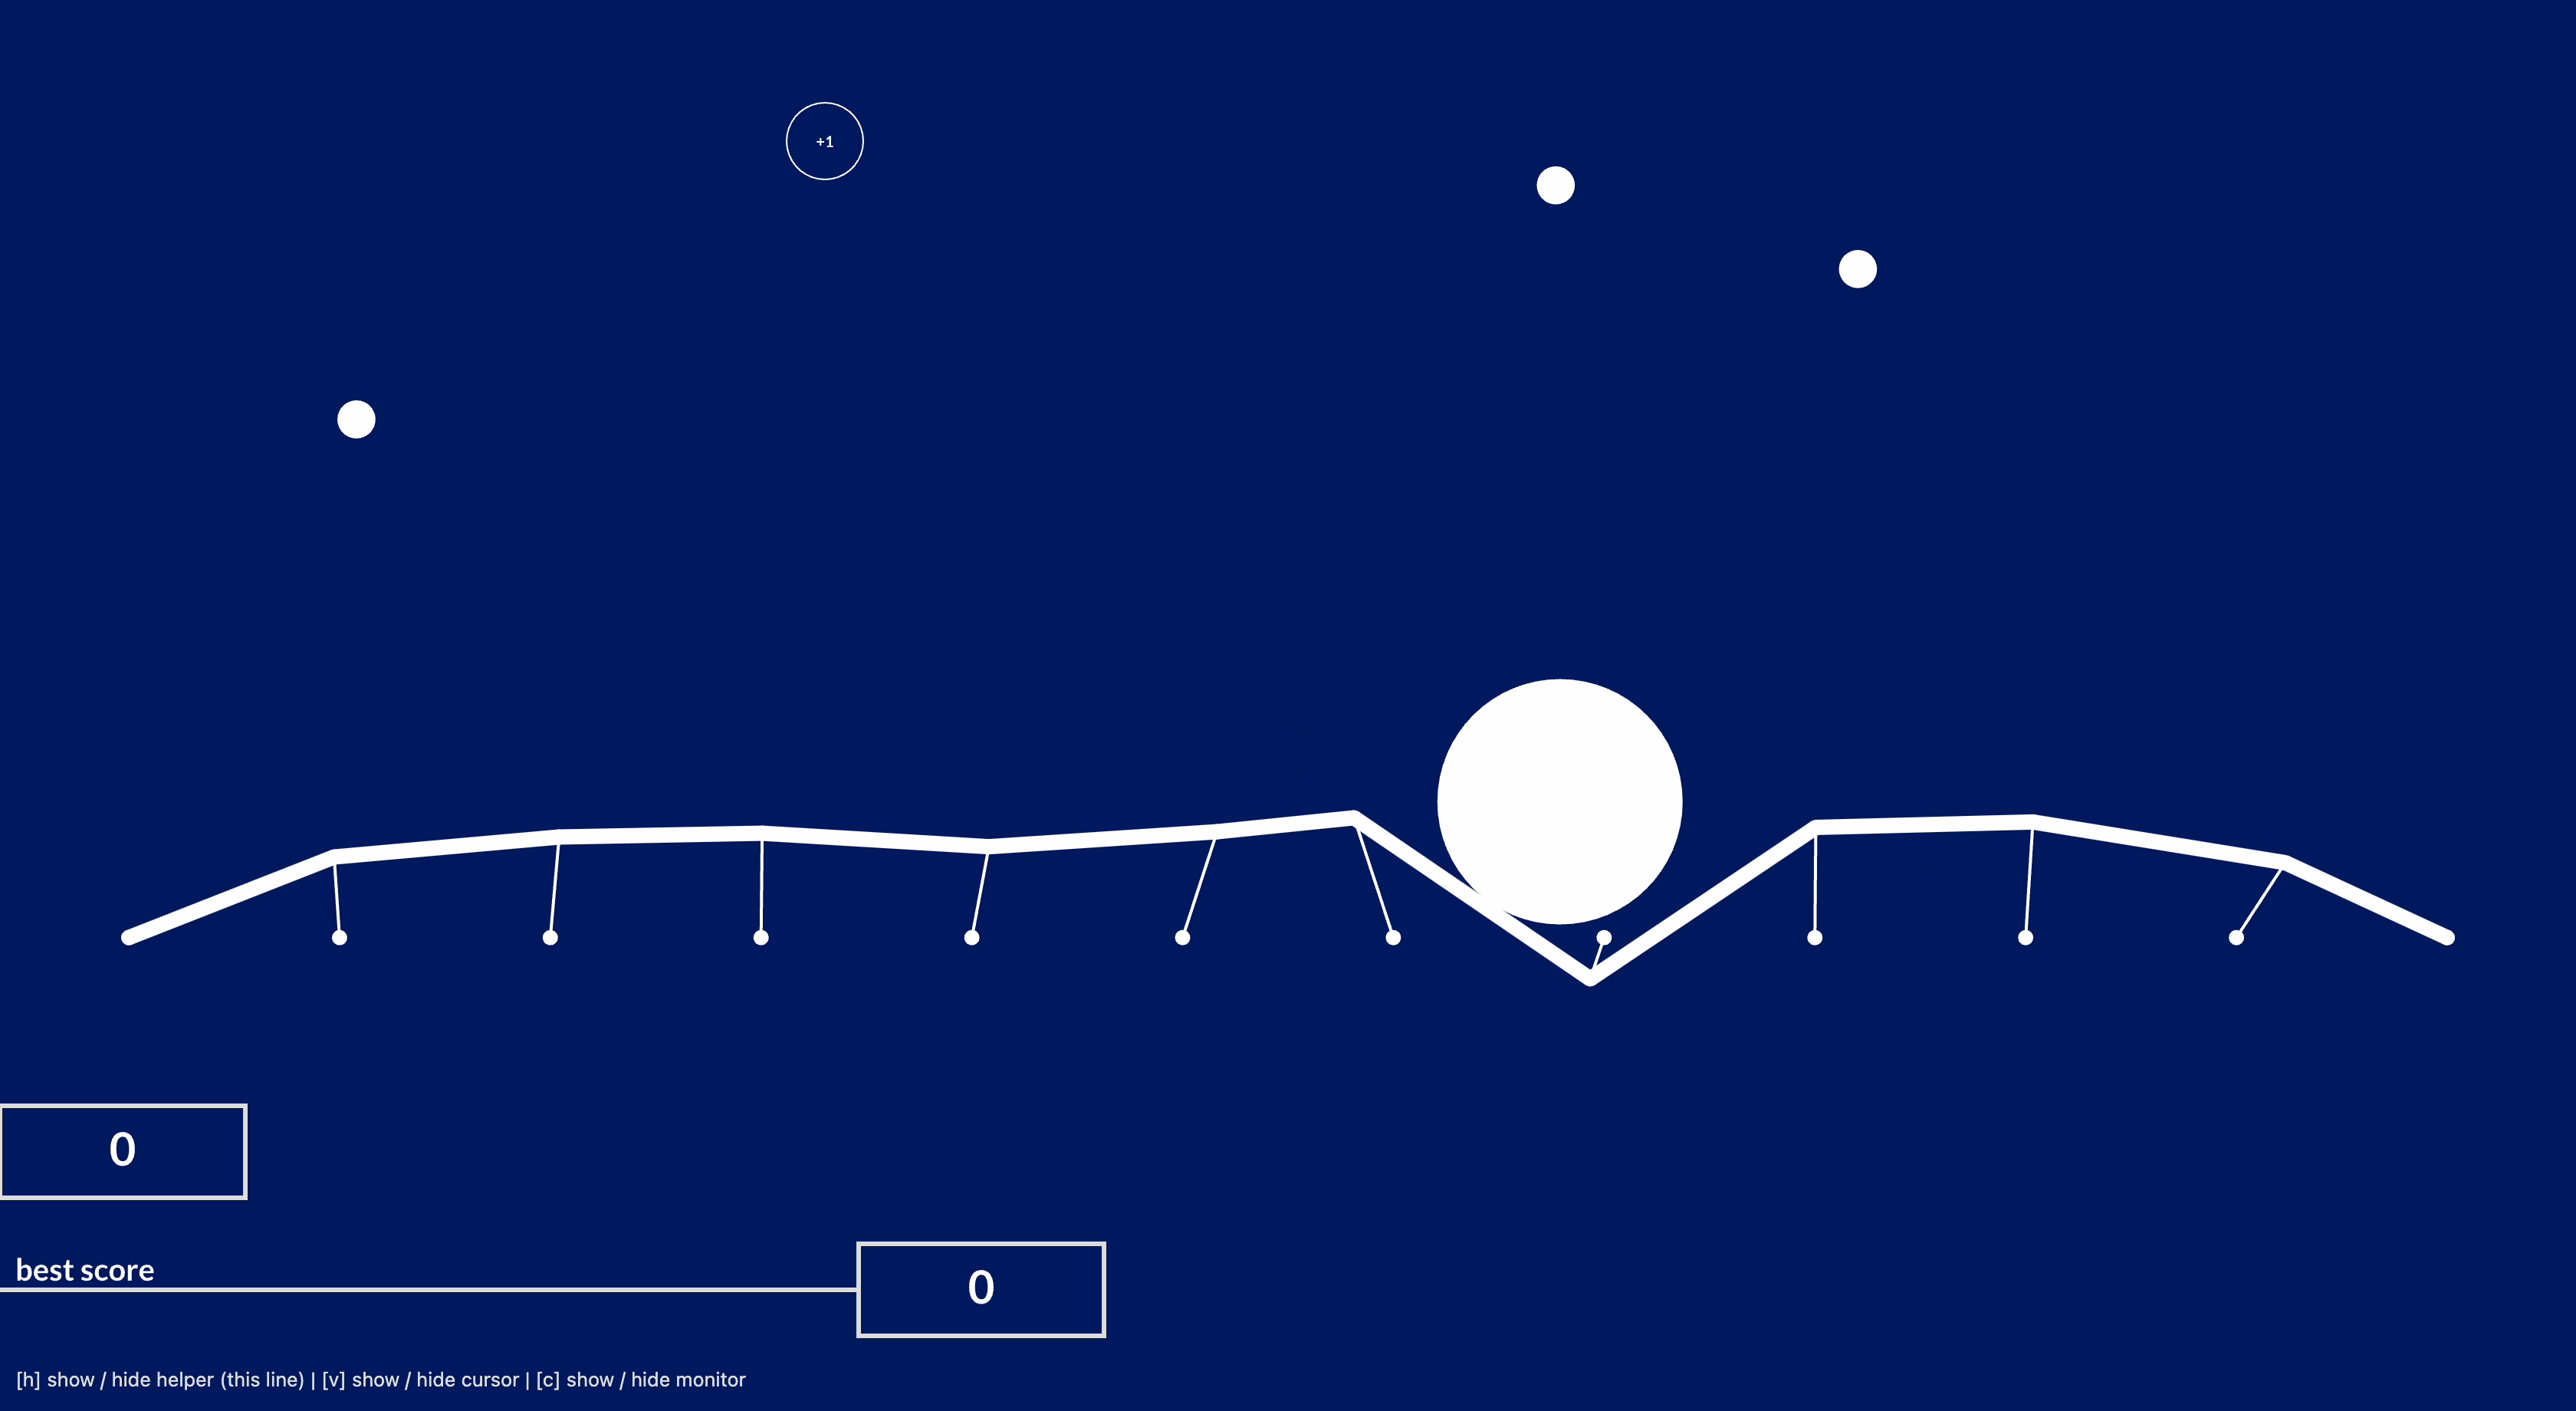
\includegraphics[width=15cm]{img/ball_overview.png}
  \caption{ボール操作の例}
  \label{fig:ball_overview}
\end{figure}

また、過去に制作したバリエーションを拡張する形で、ボール操作のパターンについて検討した\footnote{\url{https://interaction023.vercel.app/}, \url{https://interaction024.vercel.app/}}。

\begin{figure}[htbp]
  \begin{minipage}[b]{0.5\linewidth}
    \centering
    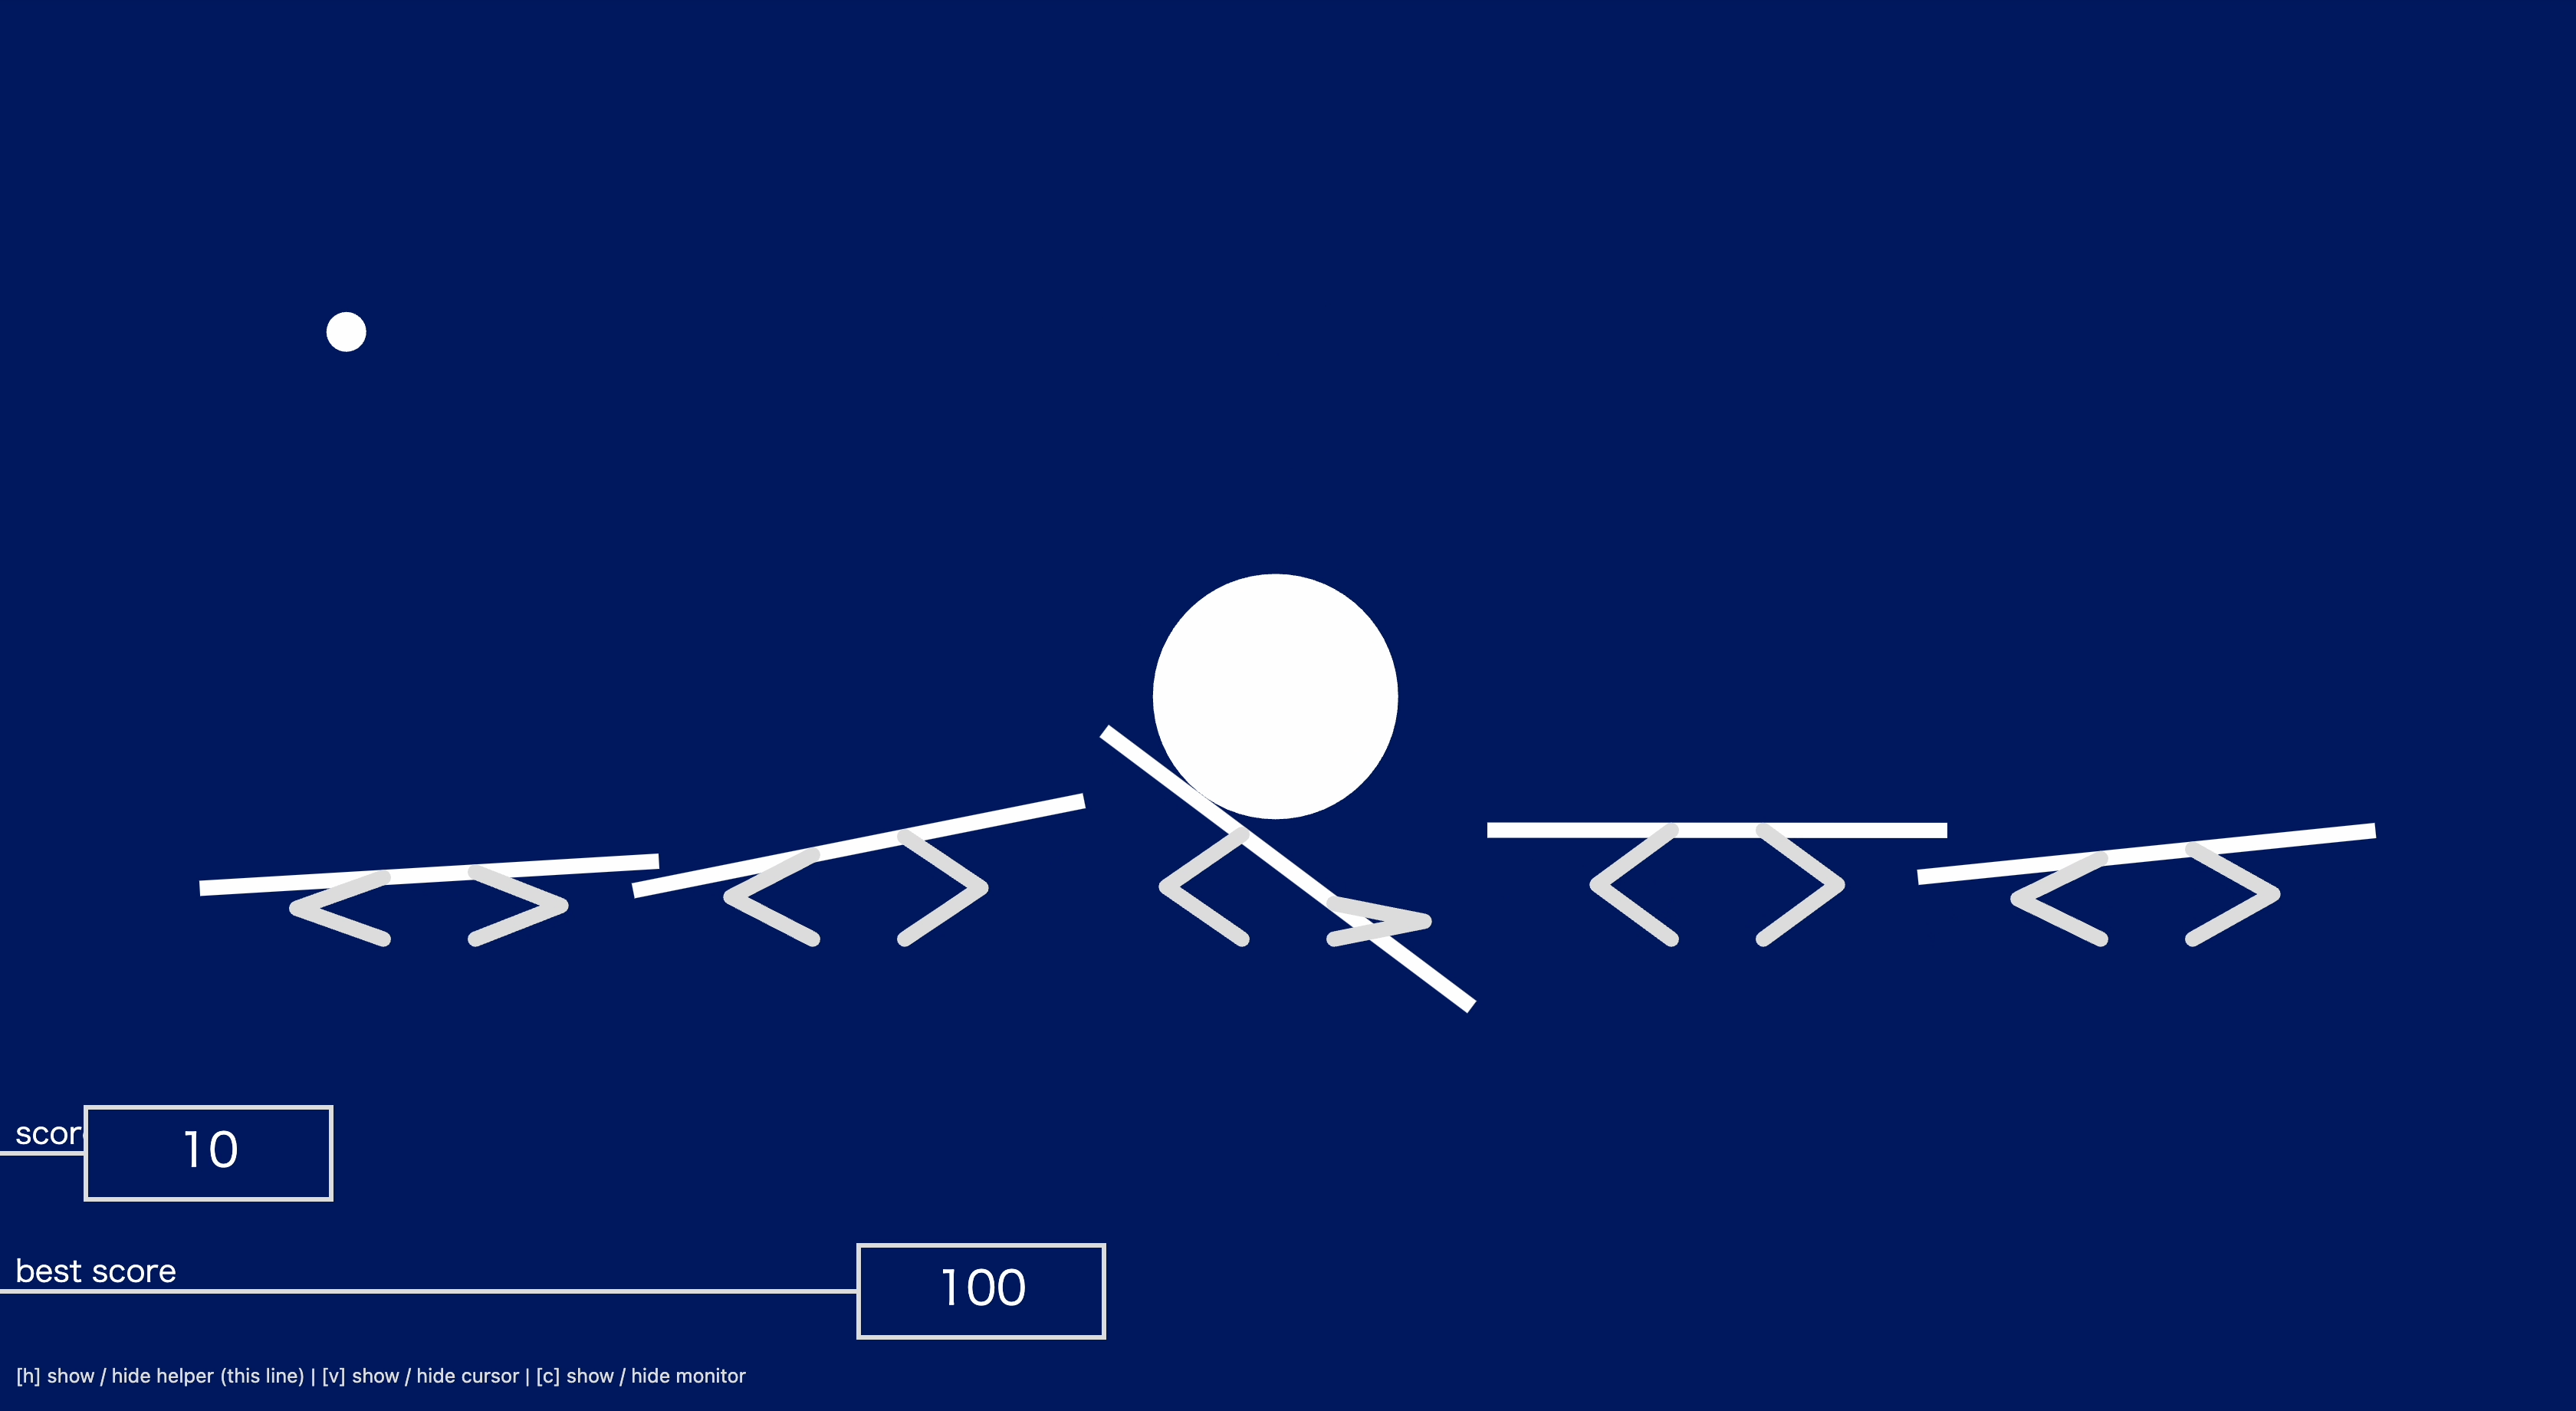
\includegraphics[keepaspectratio, width=7cm]{img/ball_0.png}
    \caption{Networked Finger}
    \label{fig:ball_0}
  \end{minipage}
  \begin{minipage}[b]{0.5\linewidth}
    \centering
    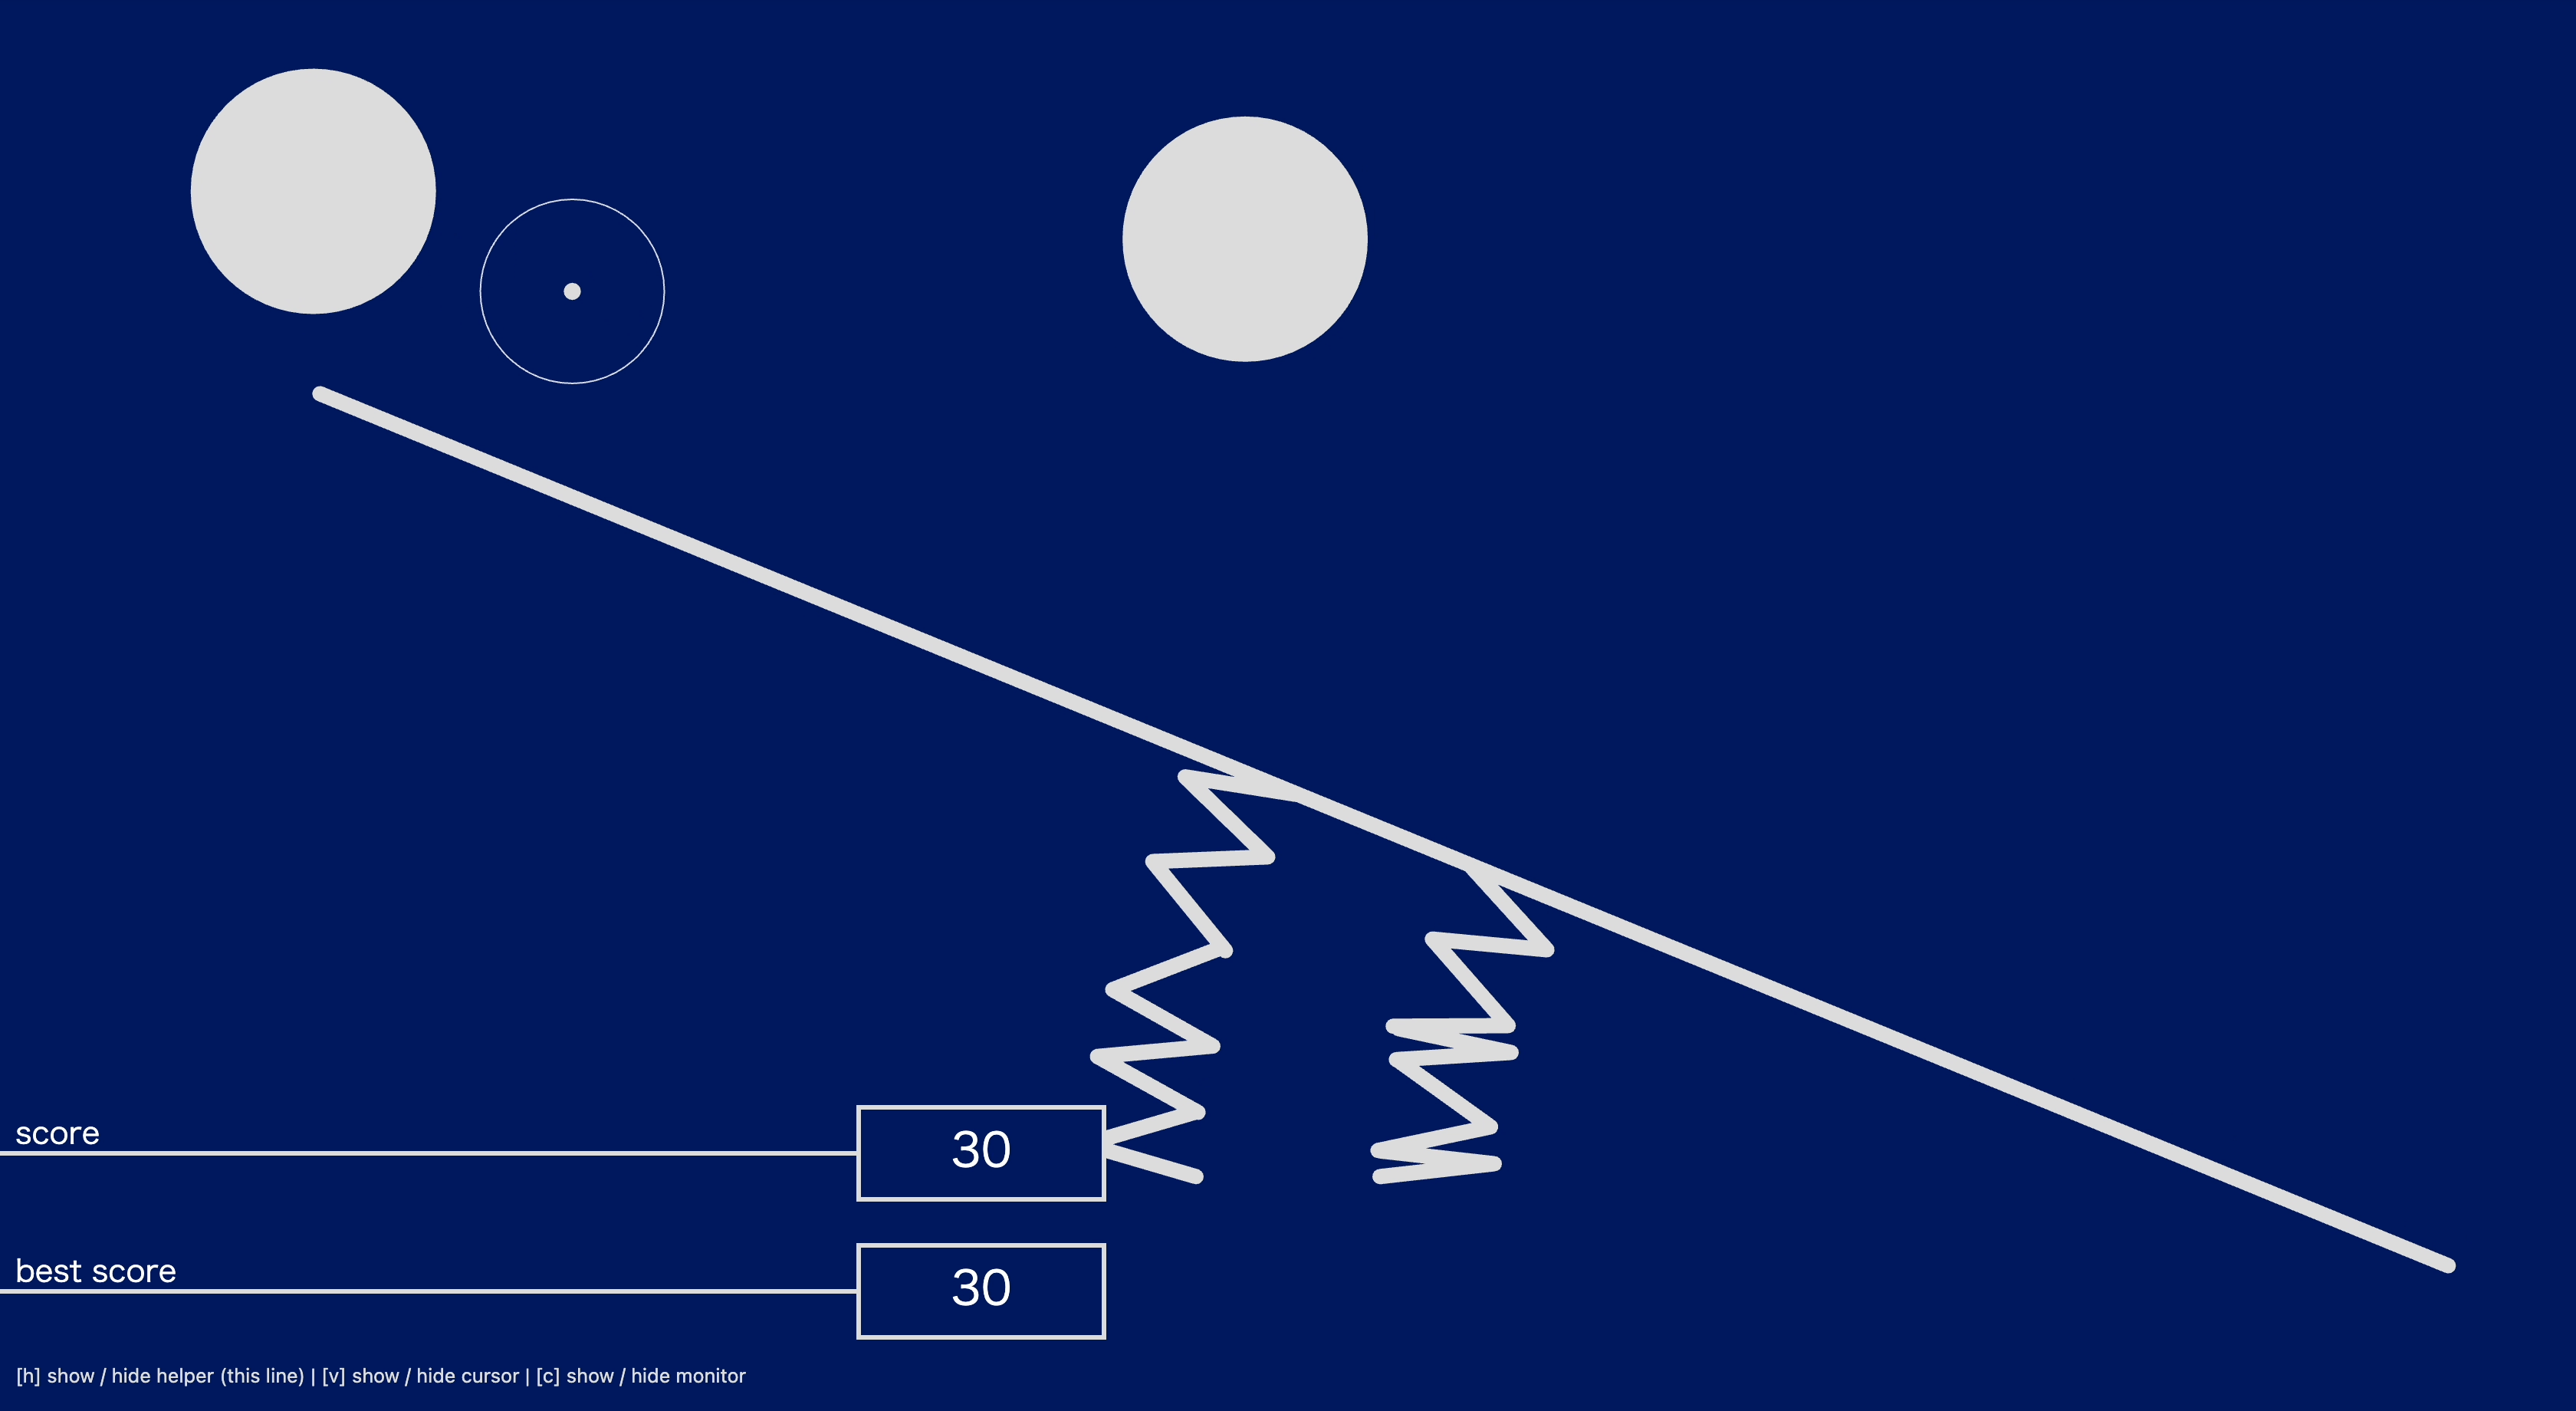
\includegraphics[keepaspectratio, width=7cm]{img/ball_1.png}
    \caption{Fractal Finger}
    \label{fig:ball_1}
  \end{minipage}
\end{figure}

\section{表現の選定}
ここまで、変換表現を扱ったプロトタイプについて概観してきた。以下では、これらのプロトタイプを踏まえて、「人馬一体感」の生起に向け、それを具現化する表現とは何か、という観点から重要だと考えられる観点を列挙し、プロトタイピングについて分析する。

\subsection{動かしている感覚が強い表現}
1つ目の観点として、手指の微細かつ複雑な動きをもって、緻密な制御をしているという感覚が引き出される表現へと絞り込んでいくことにした。

形状については、指を単位としない場合についても検討したが、指は一本一本独立して動かすことができる性質上、指が一つの単位となっている変換に注意を向けやすいのではないかと考えた。その中でも、円形、くの字、ひょうたん型などの変換を試みたが、動きに対して注意が向けられたのは「くの字」の形状であると感じられた。この理由について、身体動作である指の折り曲げとの対応から考察する。

身体動作として指の折り曲げが画面の中で、円の半径へと対応している場合とくの字のような折り曲げ動作に反応している場合とを比べたとき、後者は実際には指先と指の付け根の距離しか評価していないにも関わらず、制御点が3つあるように感じられる。そう捉えると、円の半径が変化していくことよりも対応関係が厳密であり、それを動かすことによって得られる心地よさは、Felsの「Control」による心地よさであると捉えられる。その一方で、円の半径に関節の動きをマッピングさせるような表現については、縮んだり、膨らんだりする動きには共感しづらい。微細な運動が増幅されることに気持ちよさを感じるが、これは身体動作との連動によってもたらされる気持ちよさではなく、動作に対するフィードバックに対する気持ちよさ、すなわちFelsのいう「Response」によるところが強い。

マッピングに関しては、1つの指の動きが規則的に配置される場合について、グラフィックの複雑度が上がっているにも関わらず、感覚としてはより単純な動きであると感じた。これについては、グラフィックデザイナーの女性が体験した際「構造としては緻密であるのに、動きは単純であるように感じる」と意見したことにも重なる。その理由として彼女は、「対称性が前面に出ているため、シンボルとしての印象を強く感じてしまう」「意識していないところも同時に動いている感覚があるため、自分の動きだと思えない」からではないかと推測した。一方で、不規則的に配置される図\ref{fig:networked_finger}のような形状の場合は、1つの動きが複数箇所に複製されているが、指の数が増えると複雑度も比例して上がっているように感じる。これは一つの動きが波及する箇所が多く、動きの予想がつきづらいためではないかと考える。

そのため、1つの動きを複製して円形に配置したり、フラクタル的に配置するパターンは採用しなかった。また、形状についてのバリエーションでの振り返りを通して、関節の動きが身体動作との関連について想起しやすい変換であると考え、それ以外の展開を採用しなかった。

\subsection{注意の対象による作品の分割}
ボール操作に関しては、身体動作を通して直接的に動かすことのできる対象ではないものが現れたことによって、体験の中に「もどかしさ」が生じたと考える。特に、マトのあるときが強かった。これは、明確かつ簡単に達成することのできない目標設定がされることからではないかと考える。また、マトあての利点として、「一体化」の度合いを「いかに器用にマトに当てることができたか」という観点から、客観的にも、主観的にも確かめることができると考えた。しかしその一方で、ボールの出現によって手指だけを動かして感覚を確かめていたときとは、全く異質の体験であると感じた。手指の変換のみが行われていた時には、指一本一本の動きや、それによって構成される全体的な動きに注目していたが、ボールが出現したことによってボールと手の関係性にのみ、注目するようになったと考える。

ボール操作に関するバリエーションを制作した際の気づきから、ボール操作は「もどかしさ」を経験するほどの比較的強い注意を喚起する一方で、ボールがなかった場合と比べると、注意の向く対象が、手指の運動ではなく、ボールと手指の関係性に注意が生じることがわかった。そこで、最終的な作品としてはその2つを分けて構成した。そして、手指の形状が変化することを起点に注意が生じる作品と、ボールと手指との関係性に注意が生じる作品というように、何に注意が生じるかという観点に着目して2つの体験を整理した。

また、ボールの現れる作品においては、プロトタイピングの過程で表示していた「スコア」を設けなかった。理由として、スコアが存在することで「マトに当てる」という目的意識を強く与えてしまうことが挙げられる。強固な目的意識の設計は、より多くの人を同一の目的に向かわせ、一定の体験が期待できる一方で、その目的以外の興味や注意が生じる余地を排斥してしまうと考えた。

\subsection{モーフィングの追加}
過去に展示していたバージョンではモーフィングを示さず、手指が認識されたとたんに全く違う手指が提示される作品形態であった。しかし、この形態で展示した場合、画面の中の手指と自身の関係性について意図しない受け取られ方をすることに気づいた。つまり、全く異なる生命体のようなものを、操り人形のように自分の手指の指令によって動かす、といったような関係性として認識されることがある。また、全く見慣れない形なので「手指を細かく動かせる」といった、作品がもつ可能性に気づけないことがある。そこで、形状の変化を確認できるモーフィングを実装した。そうすることで、白い点が関節を表していること、そして手指の運動を細かくトラッキングしていることを事前に伝え、それが形を変えた姿として画面の前に提示されていることがわかるようになる。

\section{展示形態の設計}
展示形態について、時系列順に過去2つのバージョンについて説明し、その流れから最終的な展示形態の根拠を示す。

\textbf{初期:カメラを画面前に配置した状態}\\
最初期は、体験装置について下図\ref{fig:kyotai_ver0}のように、モデルトラッキングを行っているカメラを直接画面の前に配置していた。
\begin{figure}[H]
  \centering
  \includegraphics[width=12cm]{img/kyotai_ver0.jpg}
  \caption{初期:カメラを画面前に配置した状態}
  \label{fig:kyotai_ver0}
\end{figure}

プロトタイピングの段階でもあったため最低限の構成としていたが、この構成には次のような問題があった。
\begin{quote}
  \begin{itemize}
    \item カメラのトラッキング精度が環境光の影響を受けて変動してしまう
    \item 体験者ではない周囲の人の手指を間違ってトラッキングしてしまう
    \item 手指の形がそのまま出力されるわけではないので、トラッキングの範囲がわからず、腕を大きく振ったり、手指がトラッキングできない範囲で動かしてしまう
  \end{itemize}
\end{quote}

このため、制作者が指示をすることなく自由に体験してもらうことを意図していた展示であっても、体験方法がわからなかったり、後方で見守る人の手を誤ってトラッキングしてしまうといった問題が起き、有効なフィードバックを得ることができなかった。

\textbf{中期:専用筐体を用いて手首を固定した状態}\\
こうした課題を踏まえて、次に専用筐体を制作し、穴に手を入れる形式について試した(図\ref{fig:kyotai_ver1})。

\begin{figure}[H]
  \centering
  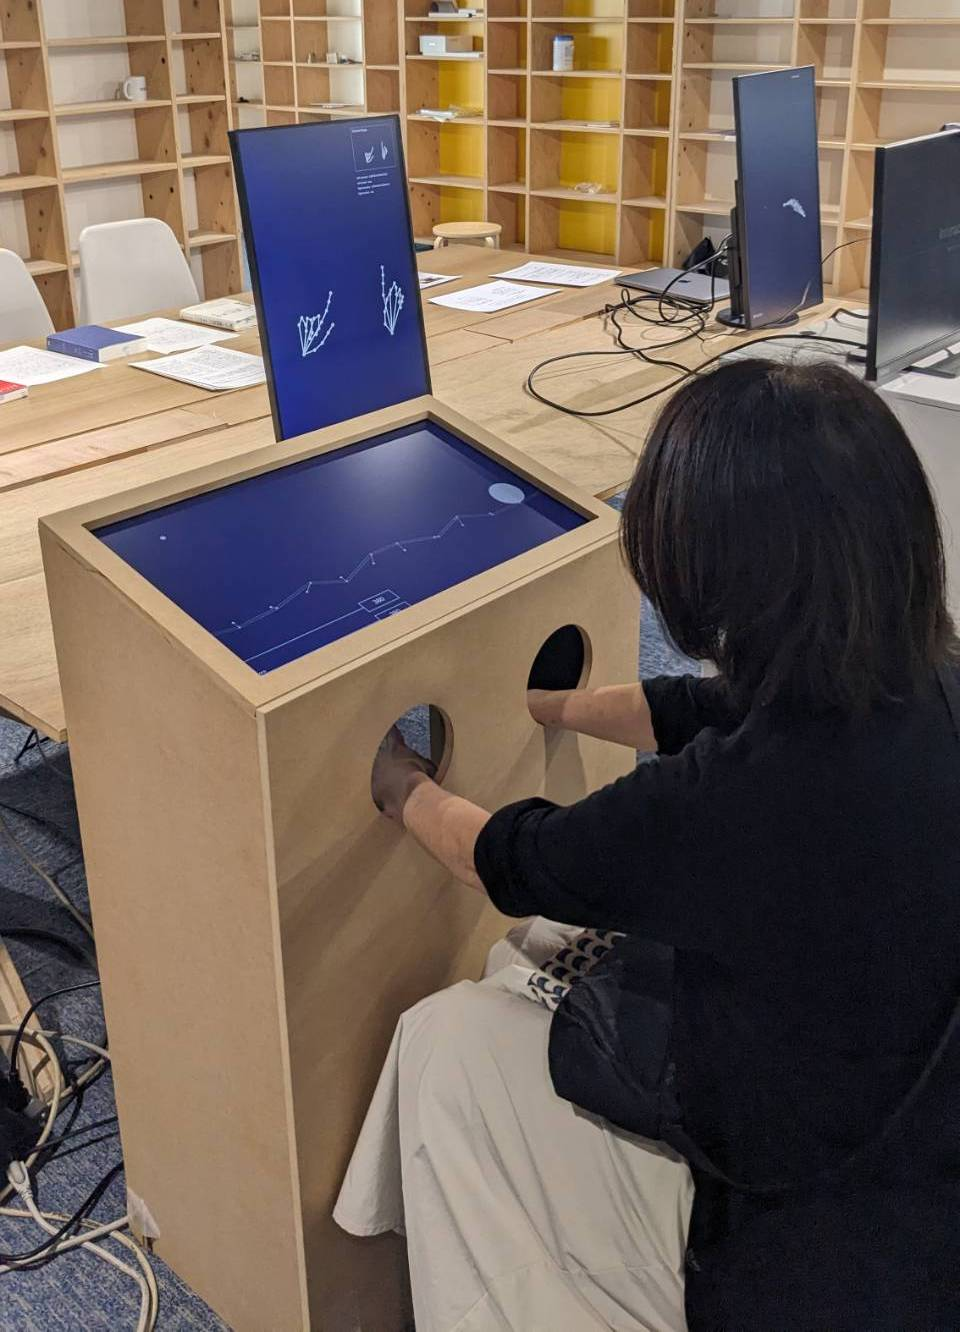
\includegraphics[width=8cm]{img/kyotai_ver1.jpg}
  \caption{中期:専用筐体を使用してカメラを隠蔽した状態}
  \label{fig:kyotai_ver1}
\end{figure}

この形式では、カメラの画角に映り込むのは筐体の内部と体験者の手のみであるため、環境光の影響や周囲の人の影響を受けずに体験できるようになった。また、穴によって手首の位置が固定されるため、腕を大きく振ることが構造上不可能となり、比較的身体動作の幅が抑えられた。

ただし、この形式は単に上記の問題を解決したというだけではなく、指先の動きが見えなくなったこと、画面に対する指先の位置関係についてを変更するものであった。

画面に対する手指の位置関係については、本作品では手指の形状が、もとの形とは全く関係のない構造へと変化するため、作品体験には大きな影響はないと判断した。手指の動きが見えなくなったことについては、画面の中の手指は体験時、自身の身体に代わる存在であるから、同時に視認できない今の形態の方がむしろ、より適した構成であると判断した。

しかしその一方で、手首の動きを固定してしまったことは、身体の動きを過剰に限定してしまう結果となった。身体の動きを限定してしまうと、何か特定の動作を求められているような説明的な構成になってしまう。そのため筐体としては、より簡素な構成が好ましいと判断した。


\textbf{作品展示:専用筐体を用いて手首を固定せず指先を自由にした状態}\\
そこで最終的には、図\ref{fig:kyotai_ver2}のような、トラッキングの範囲を暗示しながら、手首を固定しない方式に変更した。また、トラッキングに用いるカメラを、視野角150°の広角カメラ(Sanwa Supply CMS-V43BK-3)に変更し、大きく手指を動かしてもトラッキングの外れることの少ないものへと変更した。

\begin{figure}[H]
  \centering
  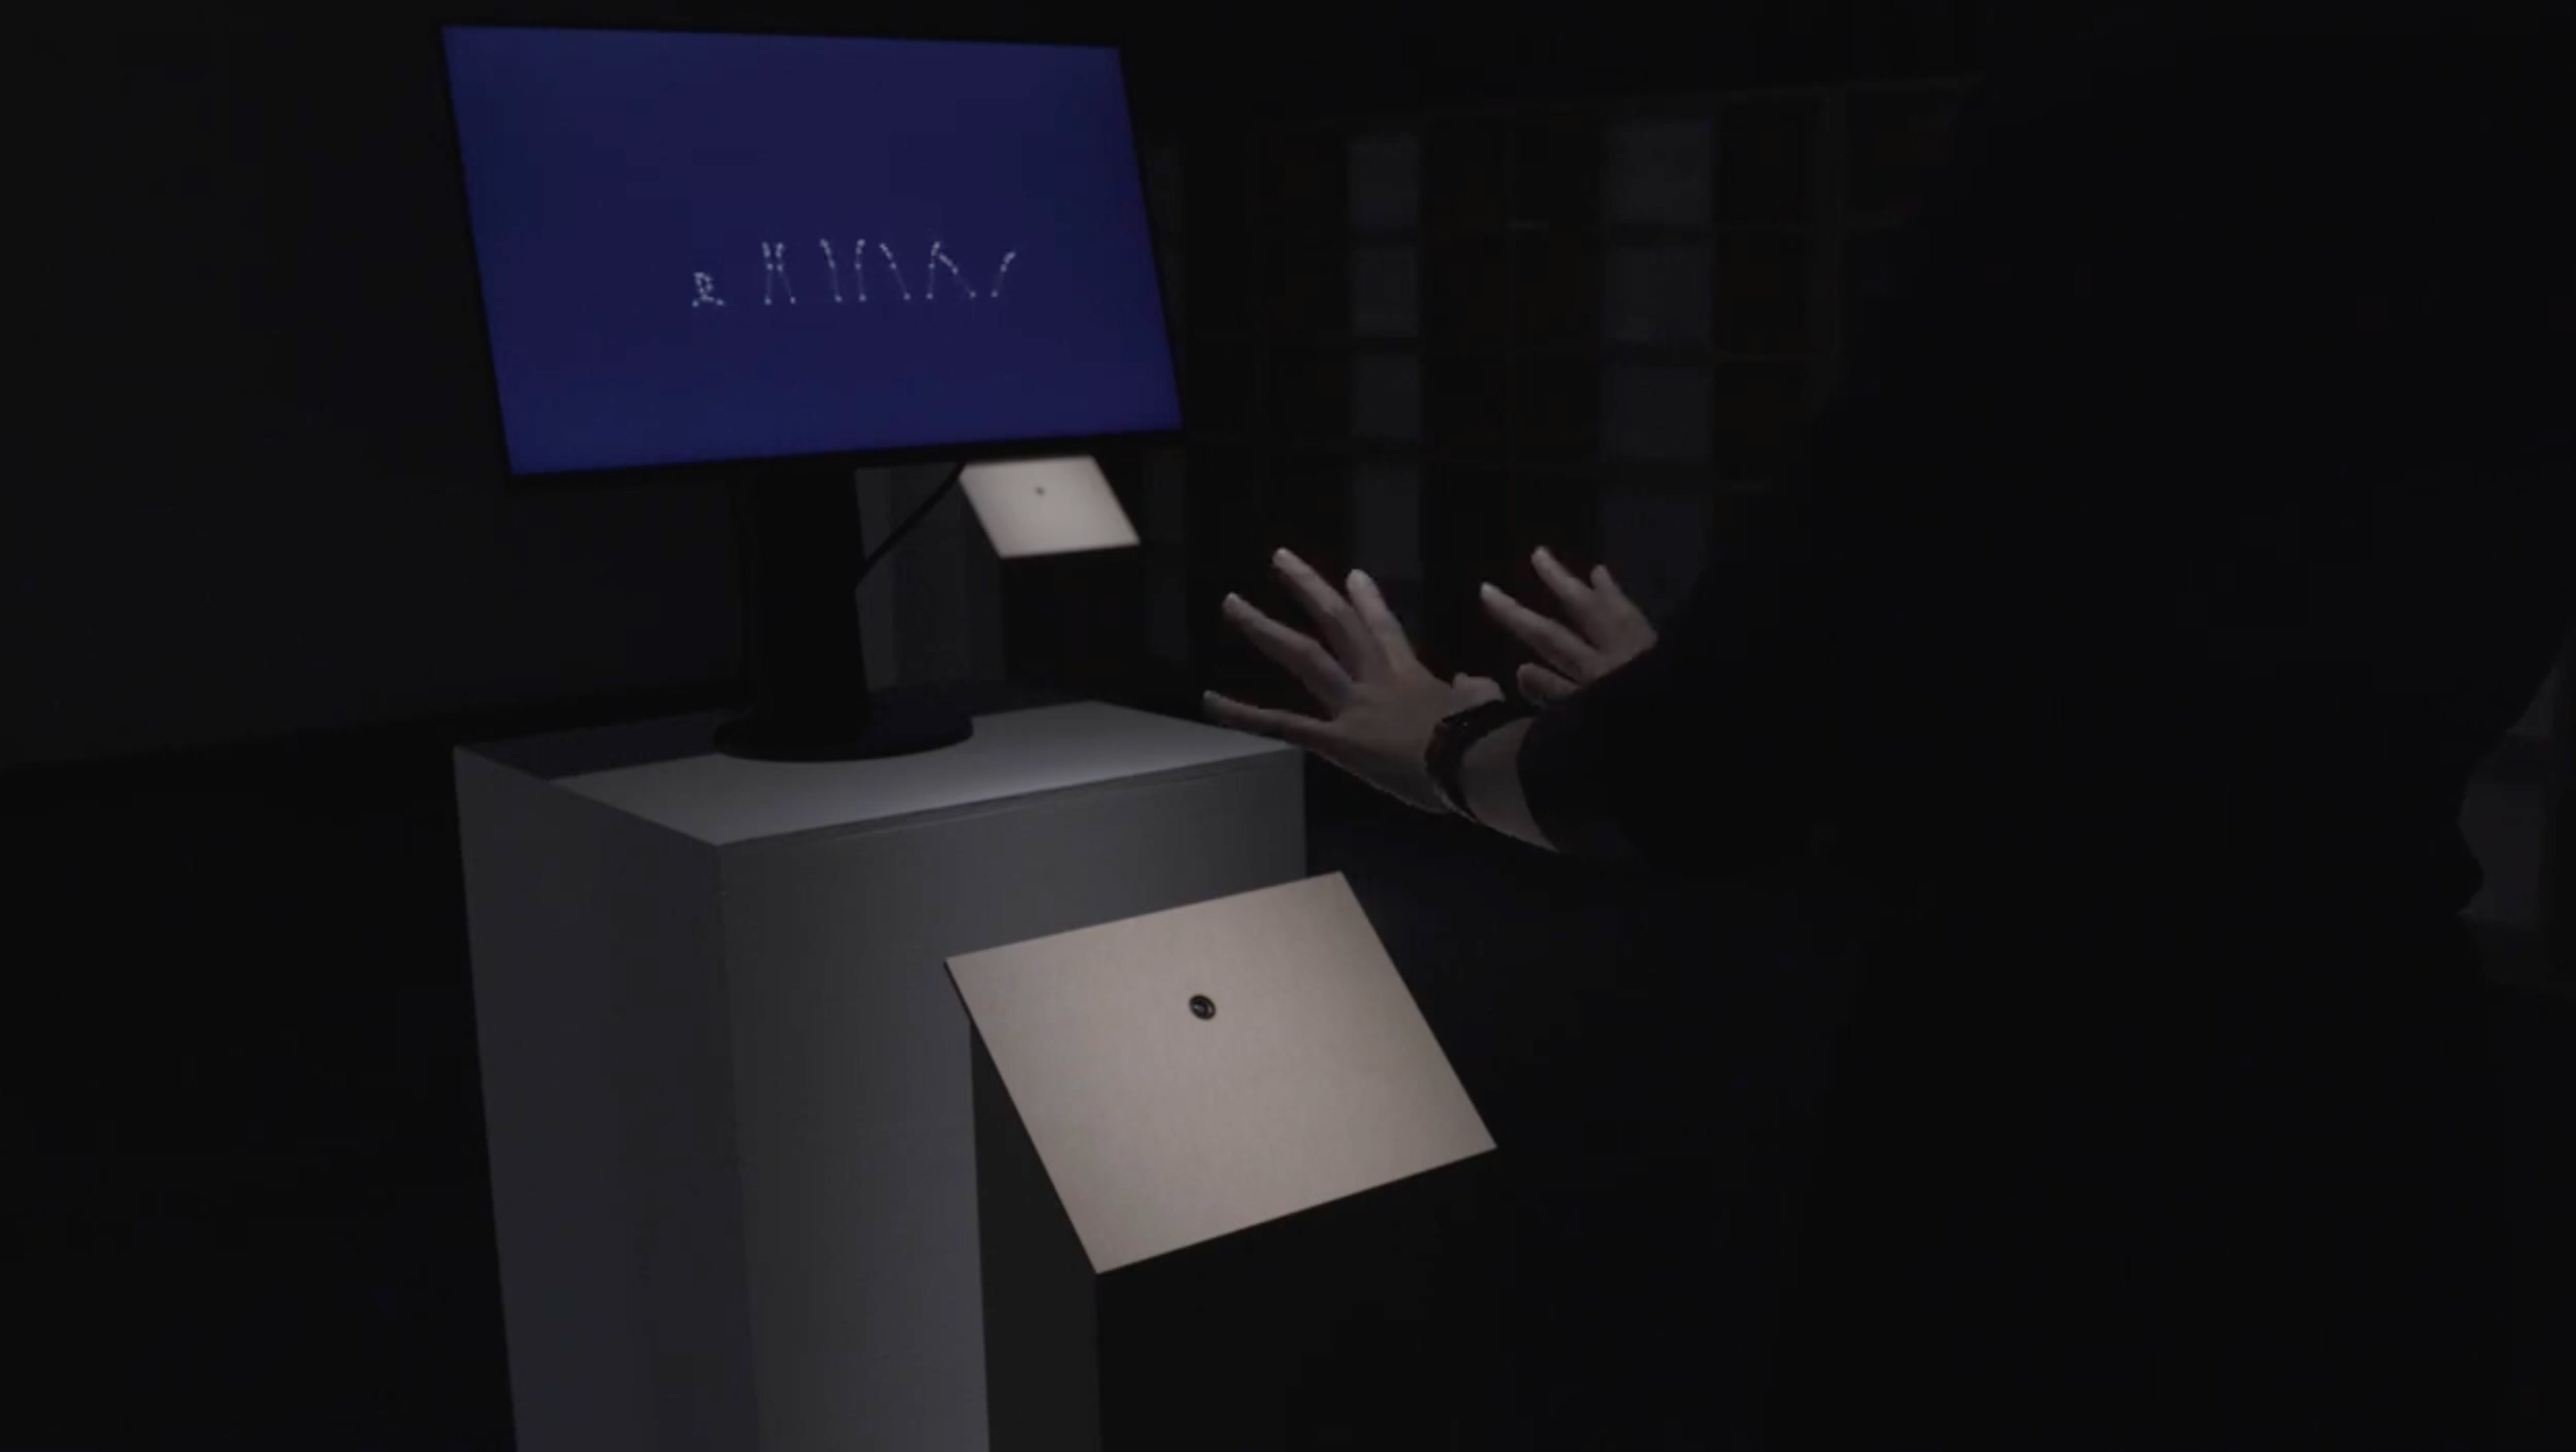
\includegraphics[width=12cm]{img/kyotai_ver2.png}
  \caption{作品展示の際の筐体}
  \label{fig:kyotai_ver2}
\end{figure}

筐体の高さは腰ほどの高さ(850mm)とすることで、キーボードのブラインドタッチのように、画面を見ながら手を同時に見ることが難しい構成とした。

カメラは、鉛直上向ではなく斜めを向いているので、筐体の前に立つと体験者の身体と手指の位置が重なり、トラッキングしやすい状況ができる。

また、ライティングの調整によってトラッキングの精度を高めた。
最終的な展示形態では、スポットライトを当てることで筐体周りを明るくすると同時に照り返しで手元の採光をし、周囲の照明を落とすことで明暗差を作ることで、手指の姿勢を認識しやすくなる。

\begin{figure}[H]
  \centering
  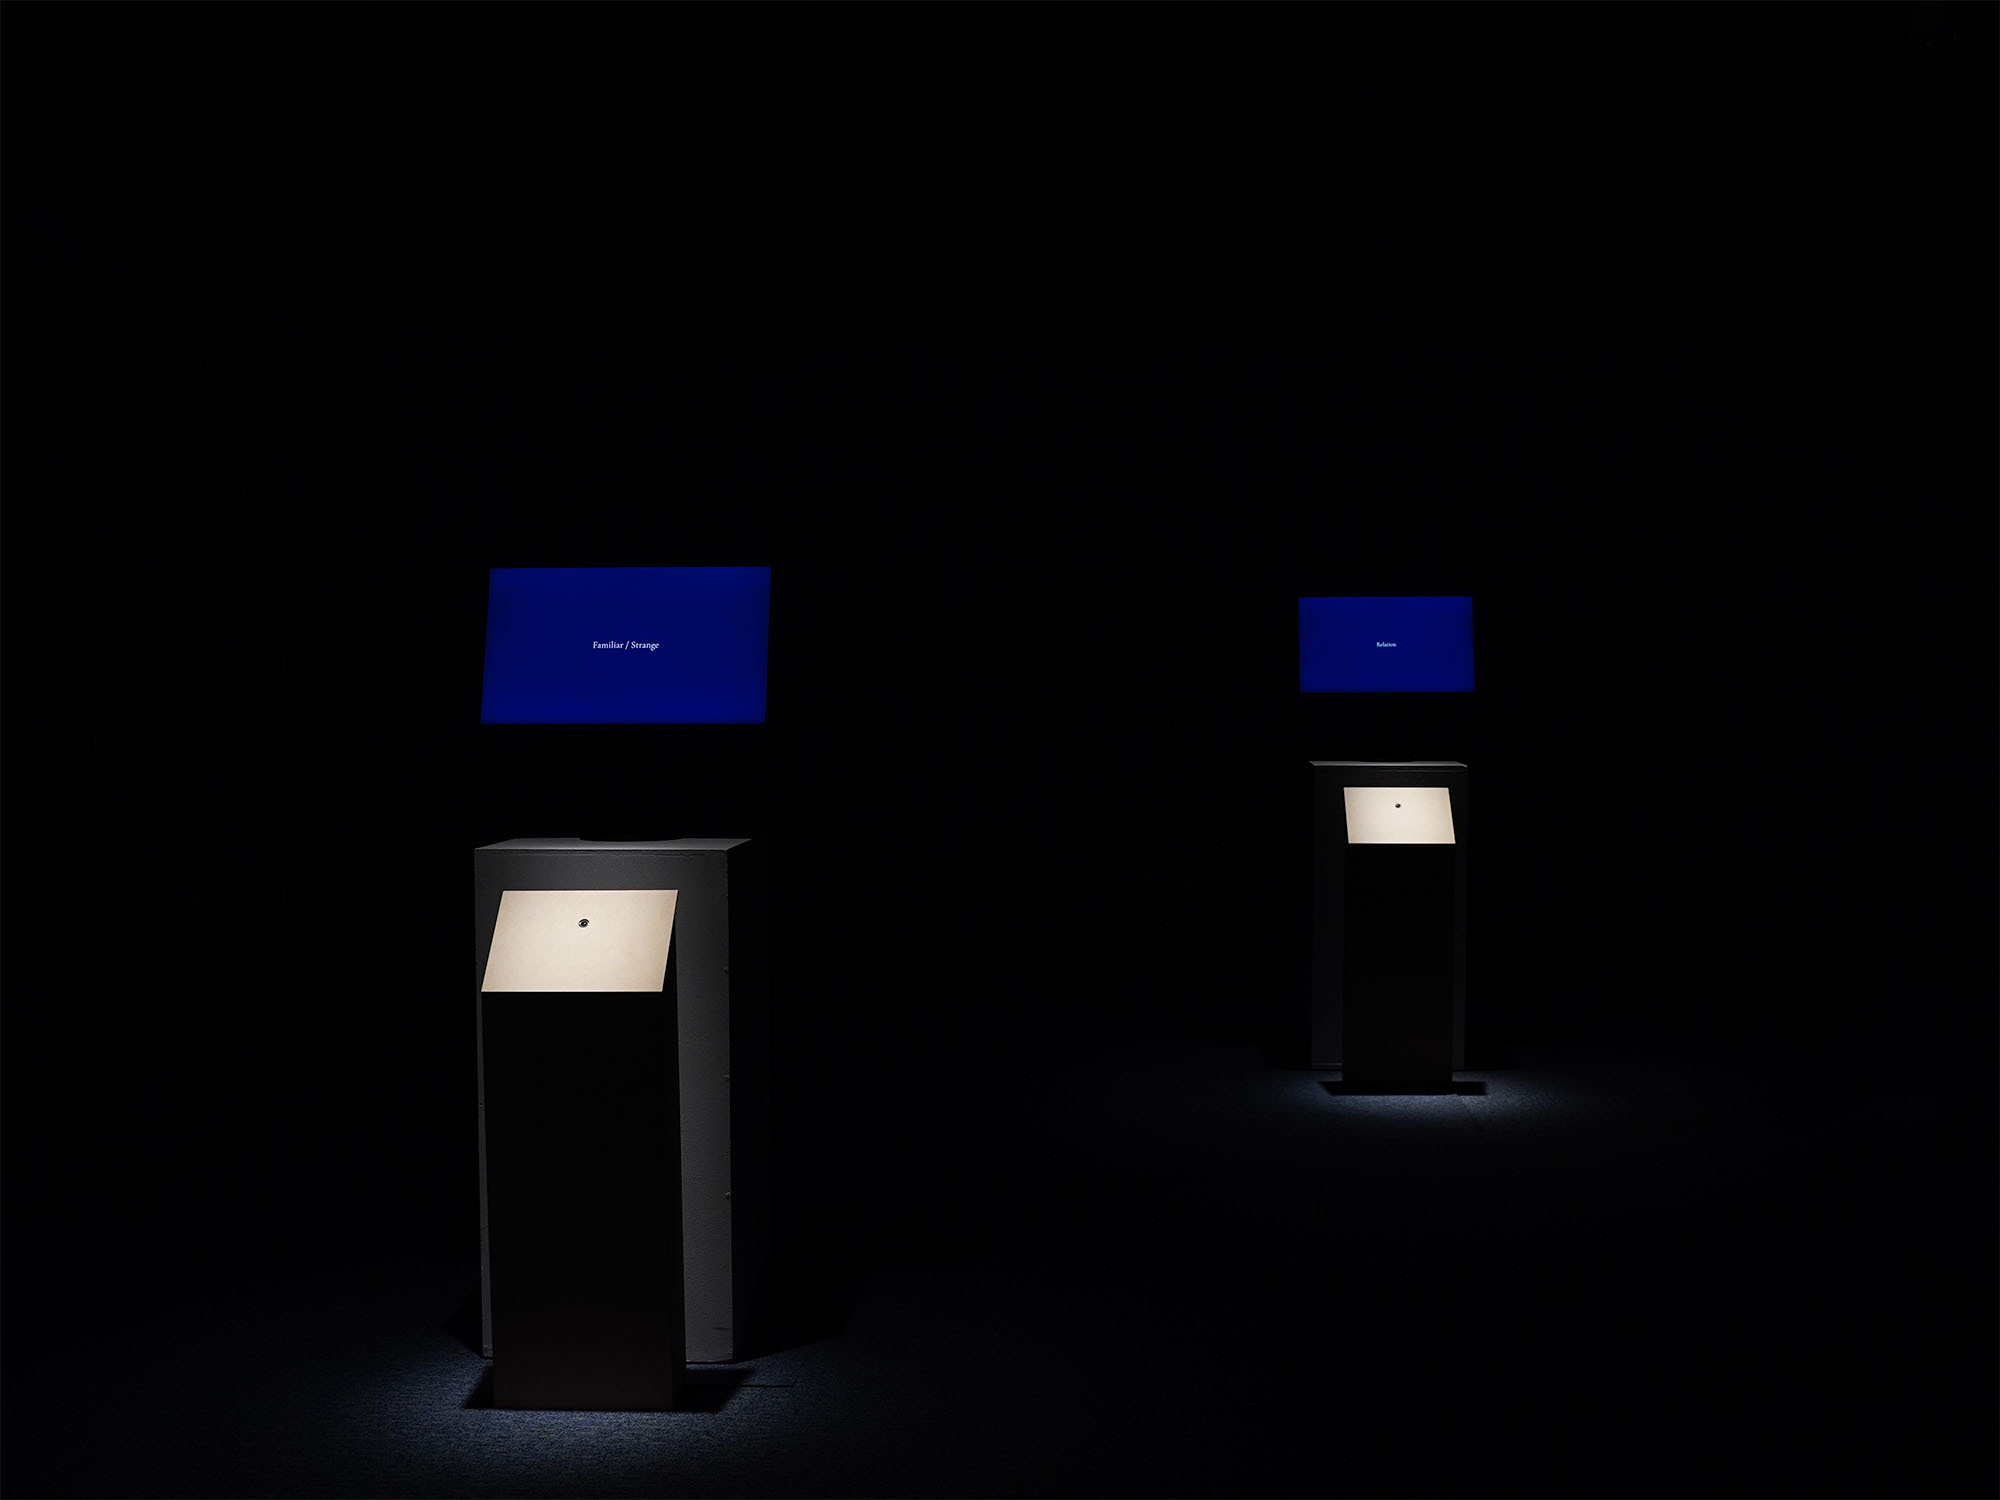
\includegraphics[width=12cm]{img/lighting.jpg}
  \caption{作品展示の際のライティング}
  \label{fig:lighting}
\end{figure}

\section{ライブラリの開発}
本作品を構成するにあたり、基本的な関数をまとめたライブラリを開発した。ライブラリには、円滑に体験するための補完処理を実装している。
具体的には、ガウシアンフィルターによる平滑化処理、トラッキングが途切れた際の例外処理の2つである。

\subsection{ガウシアンフィルターによる平滑化処理}
推定精度の問題から、モデルより推定される姿勢情報をそのまま出力すると、手指を動かしていなくても小刻みに振動したり、一時的なフレームレートの低下に起因してスムーズに動作していないように感じることがある。\\
そこで、体験者にフィードバックする際に使用する姿勢情報は、前後2フレーム分のフレーム情報にガウシアンフィルターを適用した平滑化処理を実装している。ただし、トラッキングが開始した直後は5フレーム分のフレーム情報を使用することができないため、この場合は取得できる限りのフレーム情報を用いて同じ処理を行なっている。
% そのため以下では、各フレーム情報に対する重みづけと、それを用いて体験者に提示される姿勢情報を求める上での一般式を示す。
% モデルより推定された最新の姿勢情報を\(P_{n}\)、出力されている姿勢情報を\(S\)とすると、
%   % 平滑化フレーム S の定義
%   \begin{equation}
%     S = \sum_{i=-2}^{2} w_i' \cdot P_{n+i}
%     \end{equation}

% ここで、\(w_i'\)は正規化されたガウシアンフィルタの重みを表す。正規化前の重み\(w_i\)は、
% \begin{equation}
%   w_i = \frac{1}{\sqrt{2\pi}\sigma} e^{-\frac{i^2}{2\sigma^2}}
%   \end{equation}

% 正規化された重み\(w_i'\)は、
%   % 重みの正規化
%   \begin{equation}
%   w_i' = \frac{w_i}{\sum_{j=-2}^{2} w_j}
%   \end{equation}
% と表現される。
この処理のため、最良時で60fps程度で取得される姿勢情報は、慢性的に0.3sほどの遅延を伴って体験者にフィードバックされることになる。

\subsection{トラッキングが途切れた際の例外処理}
体験時、環境光や、手指を動かす範囲や速度の関係から、トラッキングが途切れることがある。素早い動きをしている最中に1フレームでも途切れると円滑に体験することができないため、この時は例外的に、トラッキングが途切れる直前のフレーム情報で失われたフレーム情報を埋め合わせる処理を実装した。また、トラッキングが途切れていることに起因する不快感は、本作品の体験外の問題なので、手指の動きがトラッキングできていない状態を視覚的にフィードバックするため、トラッキング不能時に塗りつぶしを透過する視覚効果を実装した(\ref{fig:track_true}, \ref{fig:track_false})。

\begin{figure}[htbp]
  \begin{minipage}[b]{0.5\linewidth}
    \centering
    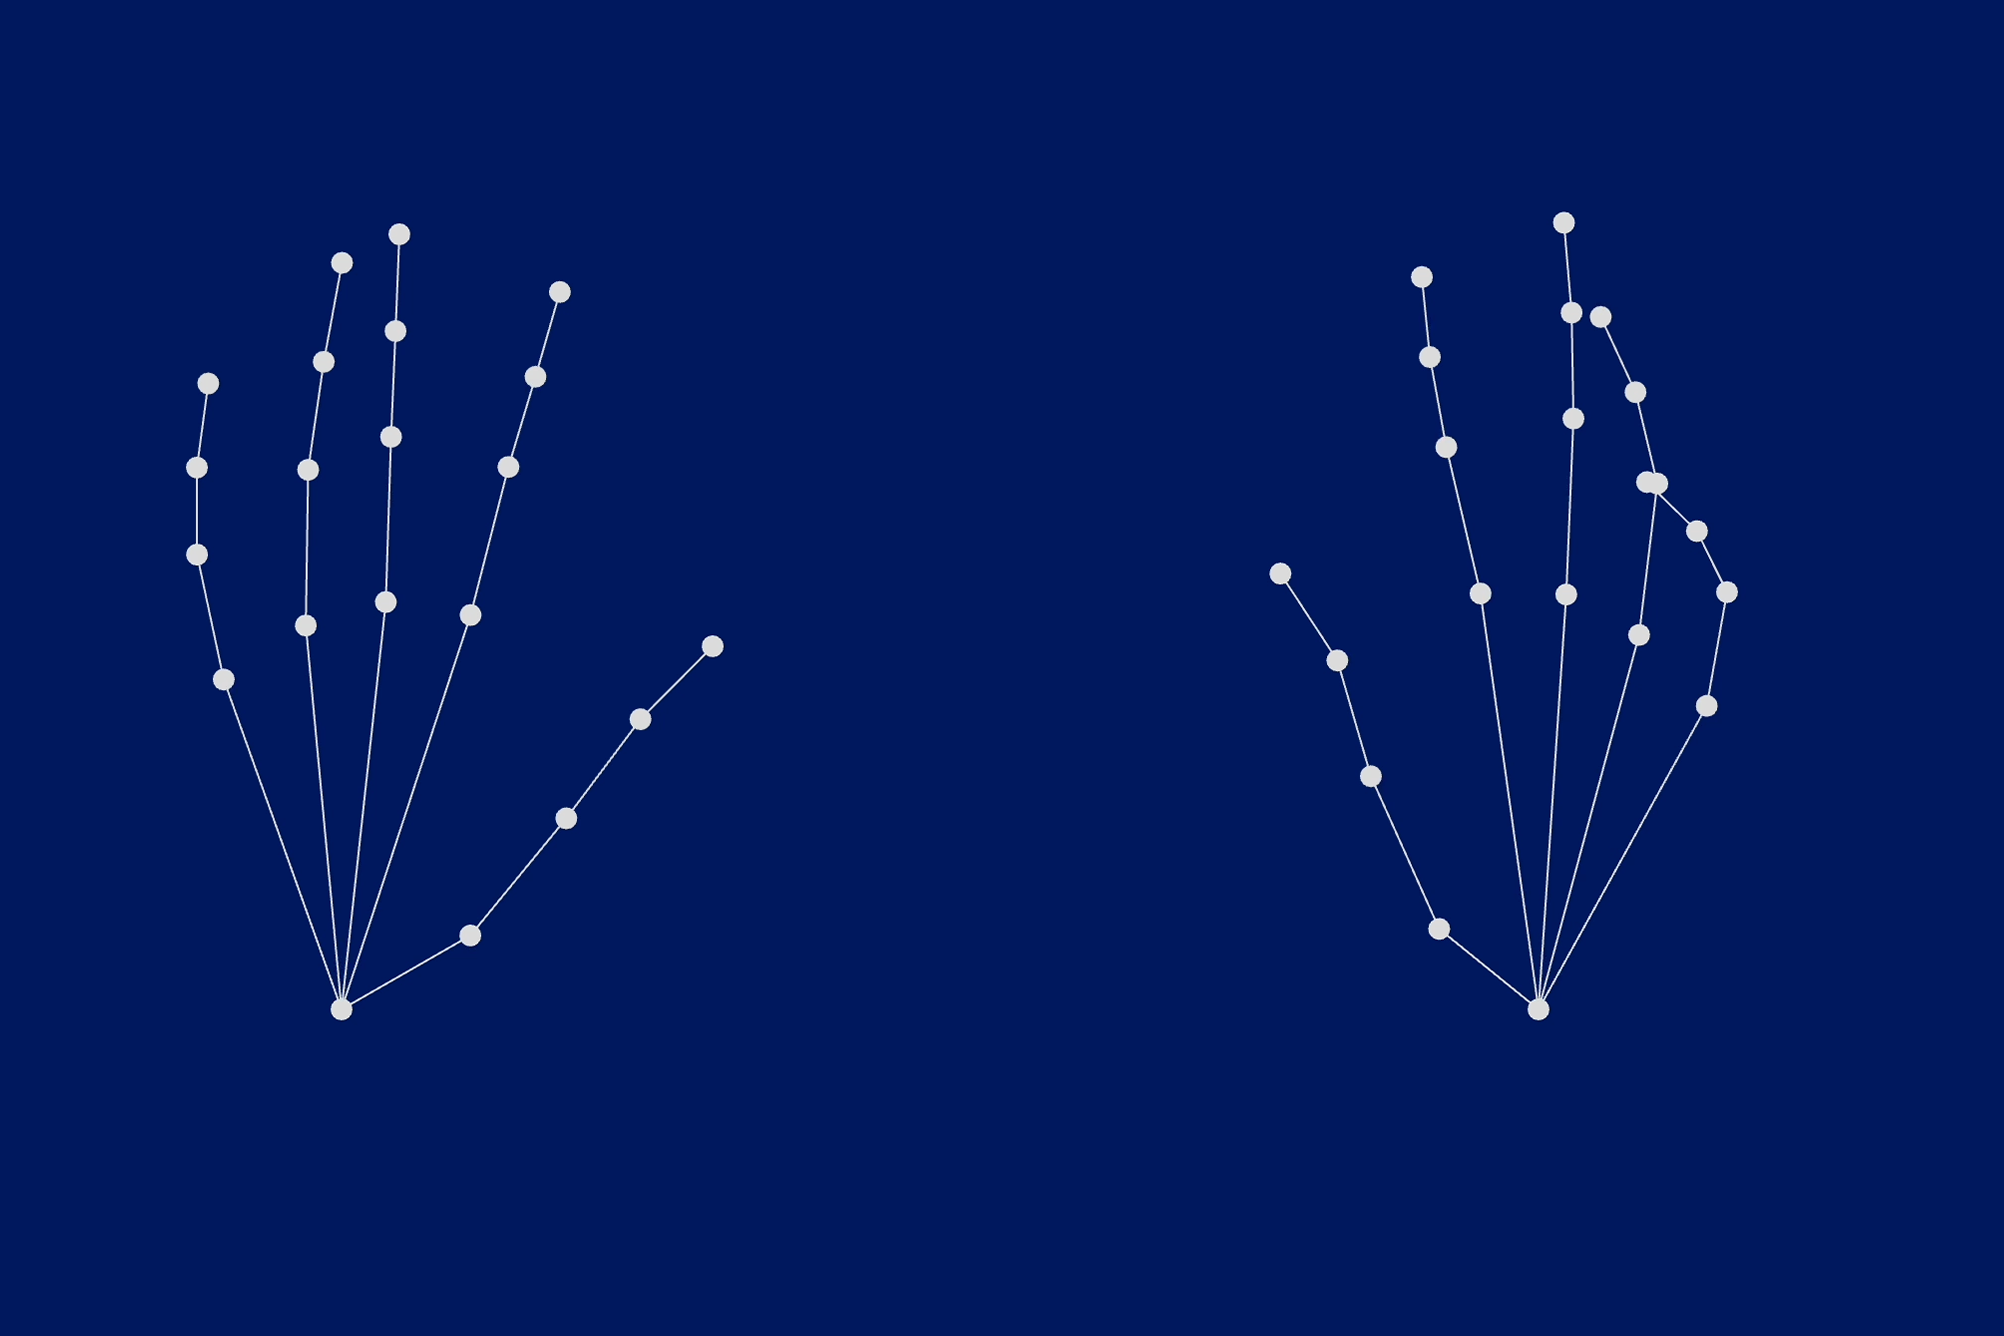
\includegraphics[keepaspectratio, width=7cm]{img/track_true.png}
    \caption{トラッキングが正常にできているとき}
    \label{fig:track_true}
  \end{minipage}
  \begin{minipage}[b]{0.5\linewidth}
    \centering
    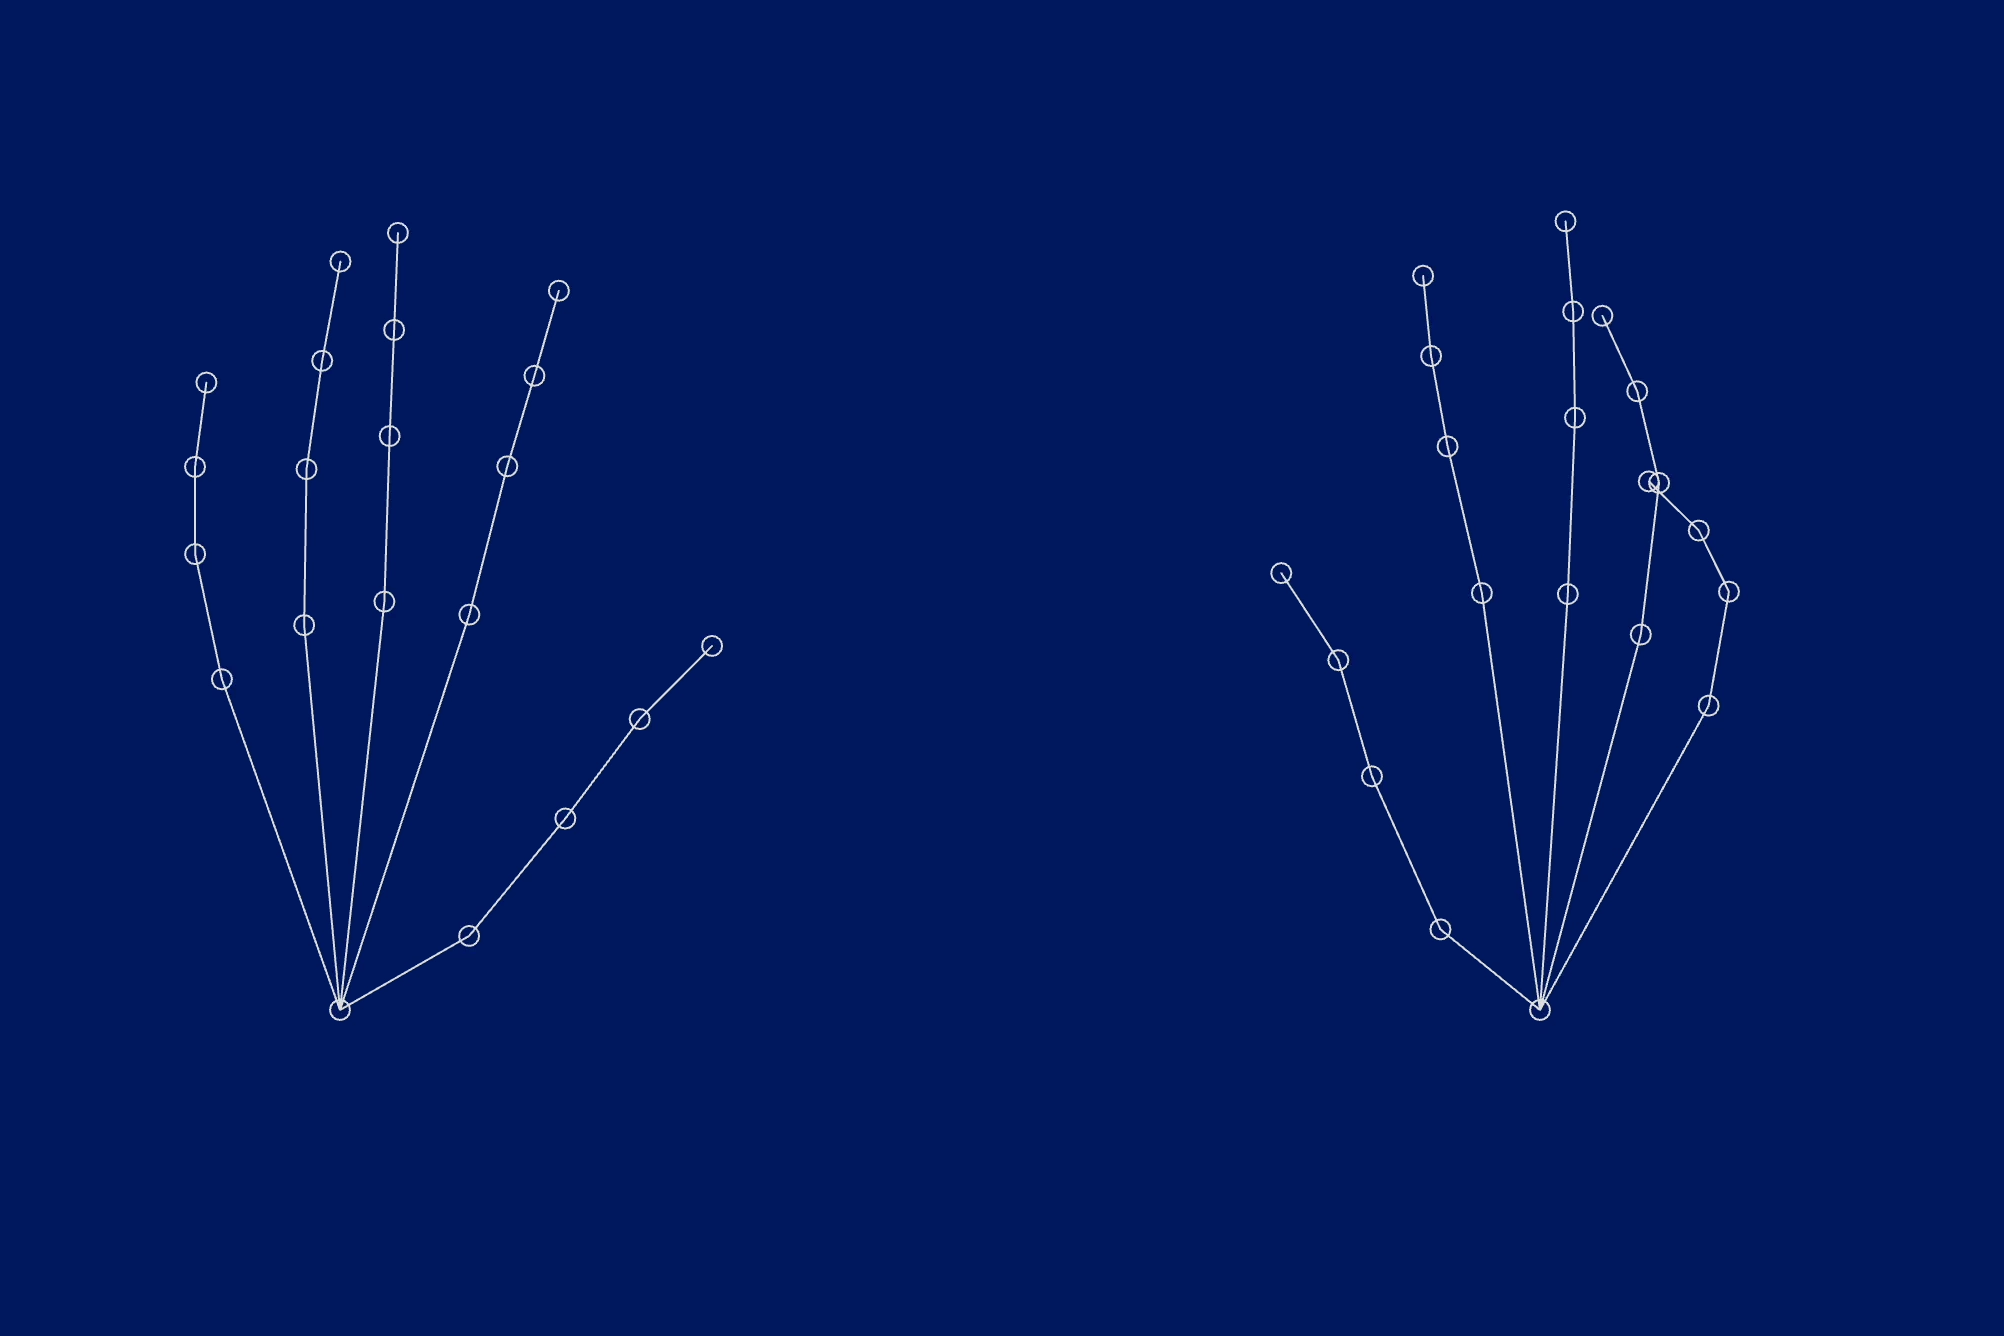
\includegraphics[keepaspectratio, width=7cm]{img/track_false.png}
    \caption{トラッキングに失敗しているとき}
    \label{fig:track_false}
  \end{minipage}
\end{figure}
\newpage
%----------------------------------------------------------------------
% 4章 実験結果 
%----------------------------------------------------------------------
\chapter{修士作品 《Grasp(er)》}
\label{about_grasper}
本章では、修士作品《Grasp(er)》の作品概要と、作品におけるねらいをSydney Felsが定義したembodimentの分類に基づいて示す。

\section{作品概要}
\begin{figure}[H]
  \centering
  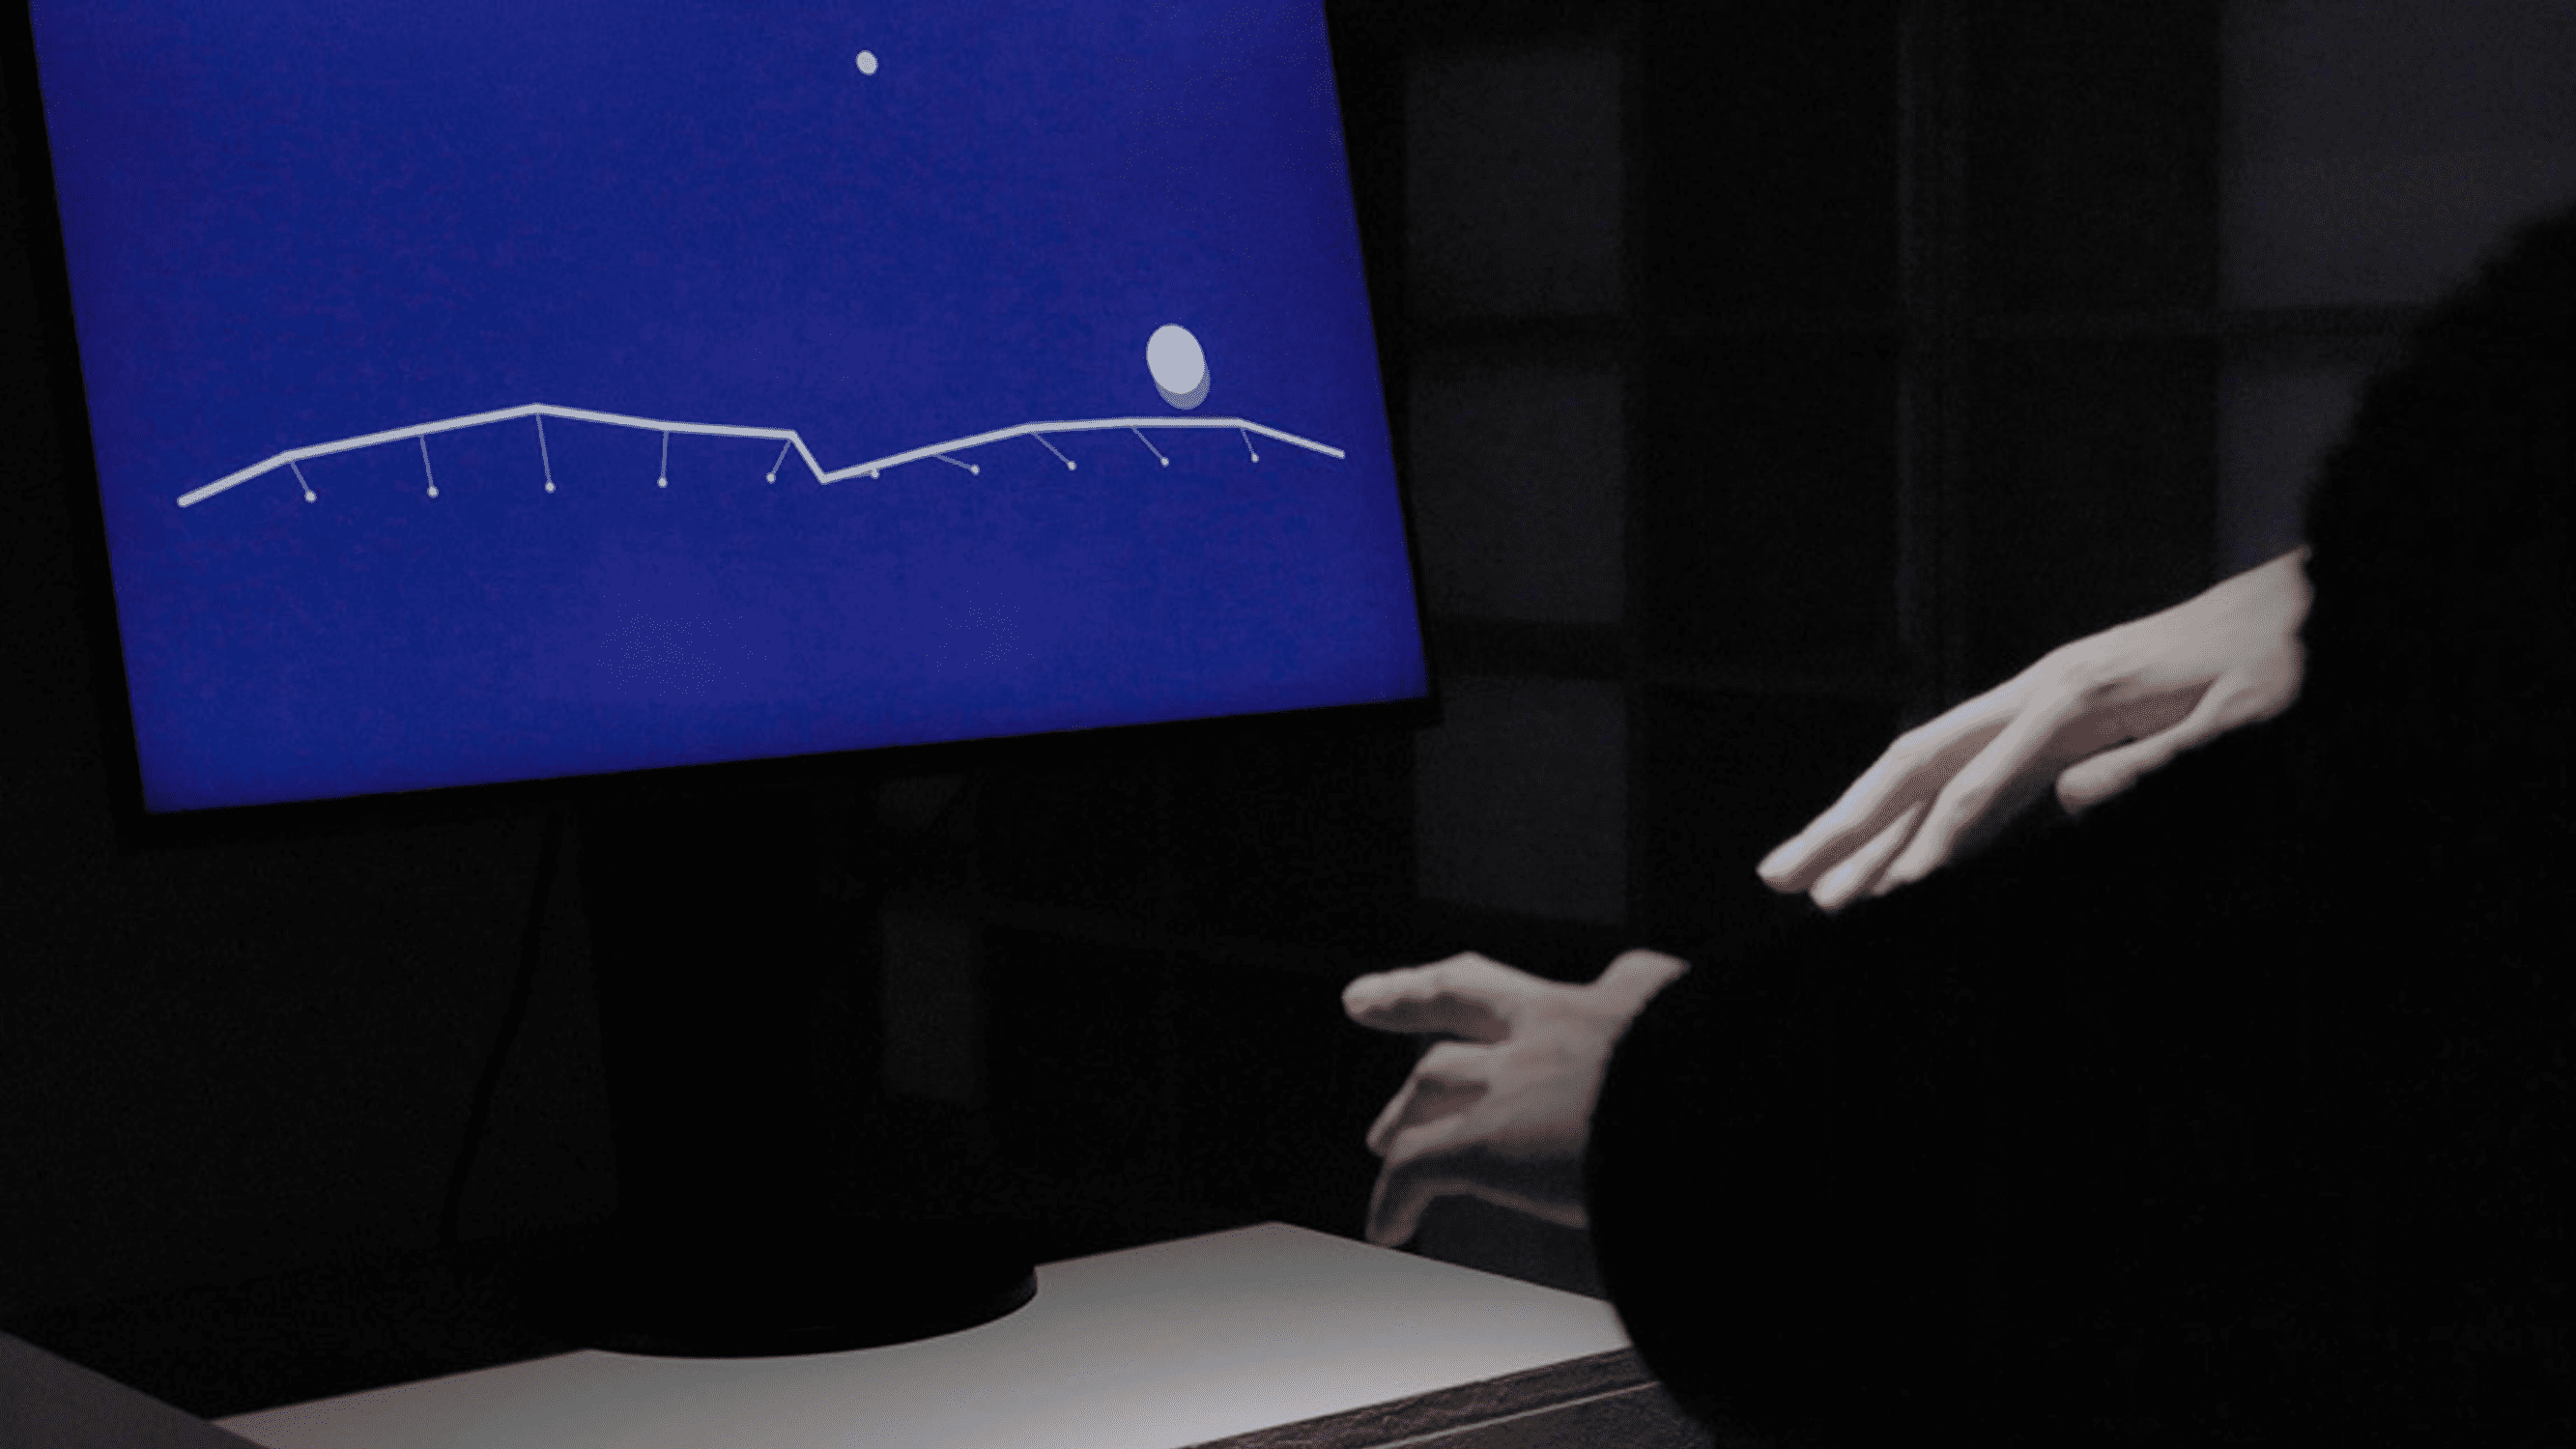
\includegraphics[width=15cm]{img/thumbnail.png}
  \caption{修士作品《Grasp(er)》}
  \label{grasper}
\end{figure}

《Grasp(er)》は、「Familiar / Strange」と「Relation」という二つから構成された作品群である。最初鏡合わせのように映った手の形が大きく変化する中で、自身の身体と手指の関係がわからなくなりながらも、注意を向けて探索的に手指を動かしていると、体の動きと画面の中の動きが一致するような感覚が芽生える。また、形の変わった手指を使って緻密な動きをする中、最初はうまくいかずもどかしさを感じながらも、試行錯誤を経て一体感が芽生えるようになる。このように《Grasp(er)》では、体験の中で意識的に調和する感覚を掴み取り、一体となる感覚を目指した。

以下では、本作を構成する2つの作品について説明する。

% これらに共通するのは、\textit{grasp}の中で個人が目的意識や興味を抱くことで、\textit{grasp}が連鎖的に生じることである。

% 制作者は「このようなことをしてほしい」という行為の中身を設計せず、体験する個人がその中で次々と注目する対象を見出すことによって、個人が行為を創造していくことを目指している。このため、「手指の構造や、手指を取り巻く環境を変化させることで、手指の運動に注目する構造」を作ることに取り組んだ。このときの「注目」が起点となって\textit{grasp}の期間が生じるが、その先々で起こる体験は個人に委ねられ、明示的な目的は設定されていない。

\subsection*{Familiar / Strange}
\begin{figure}[H]
  \centering
  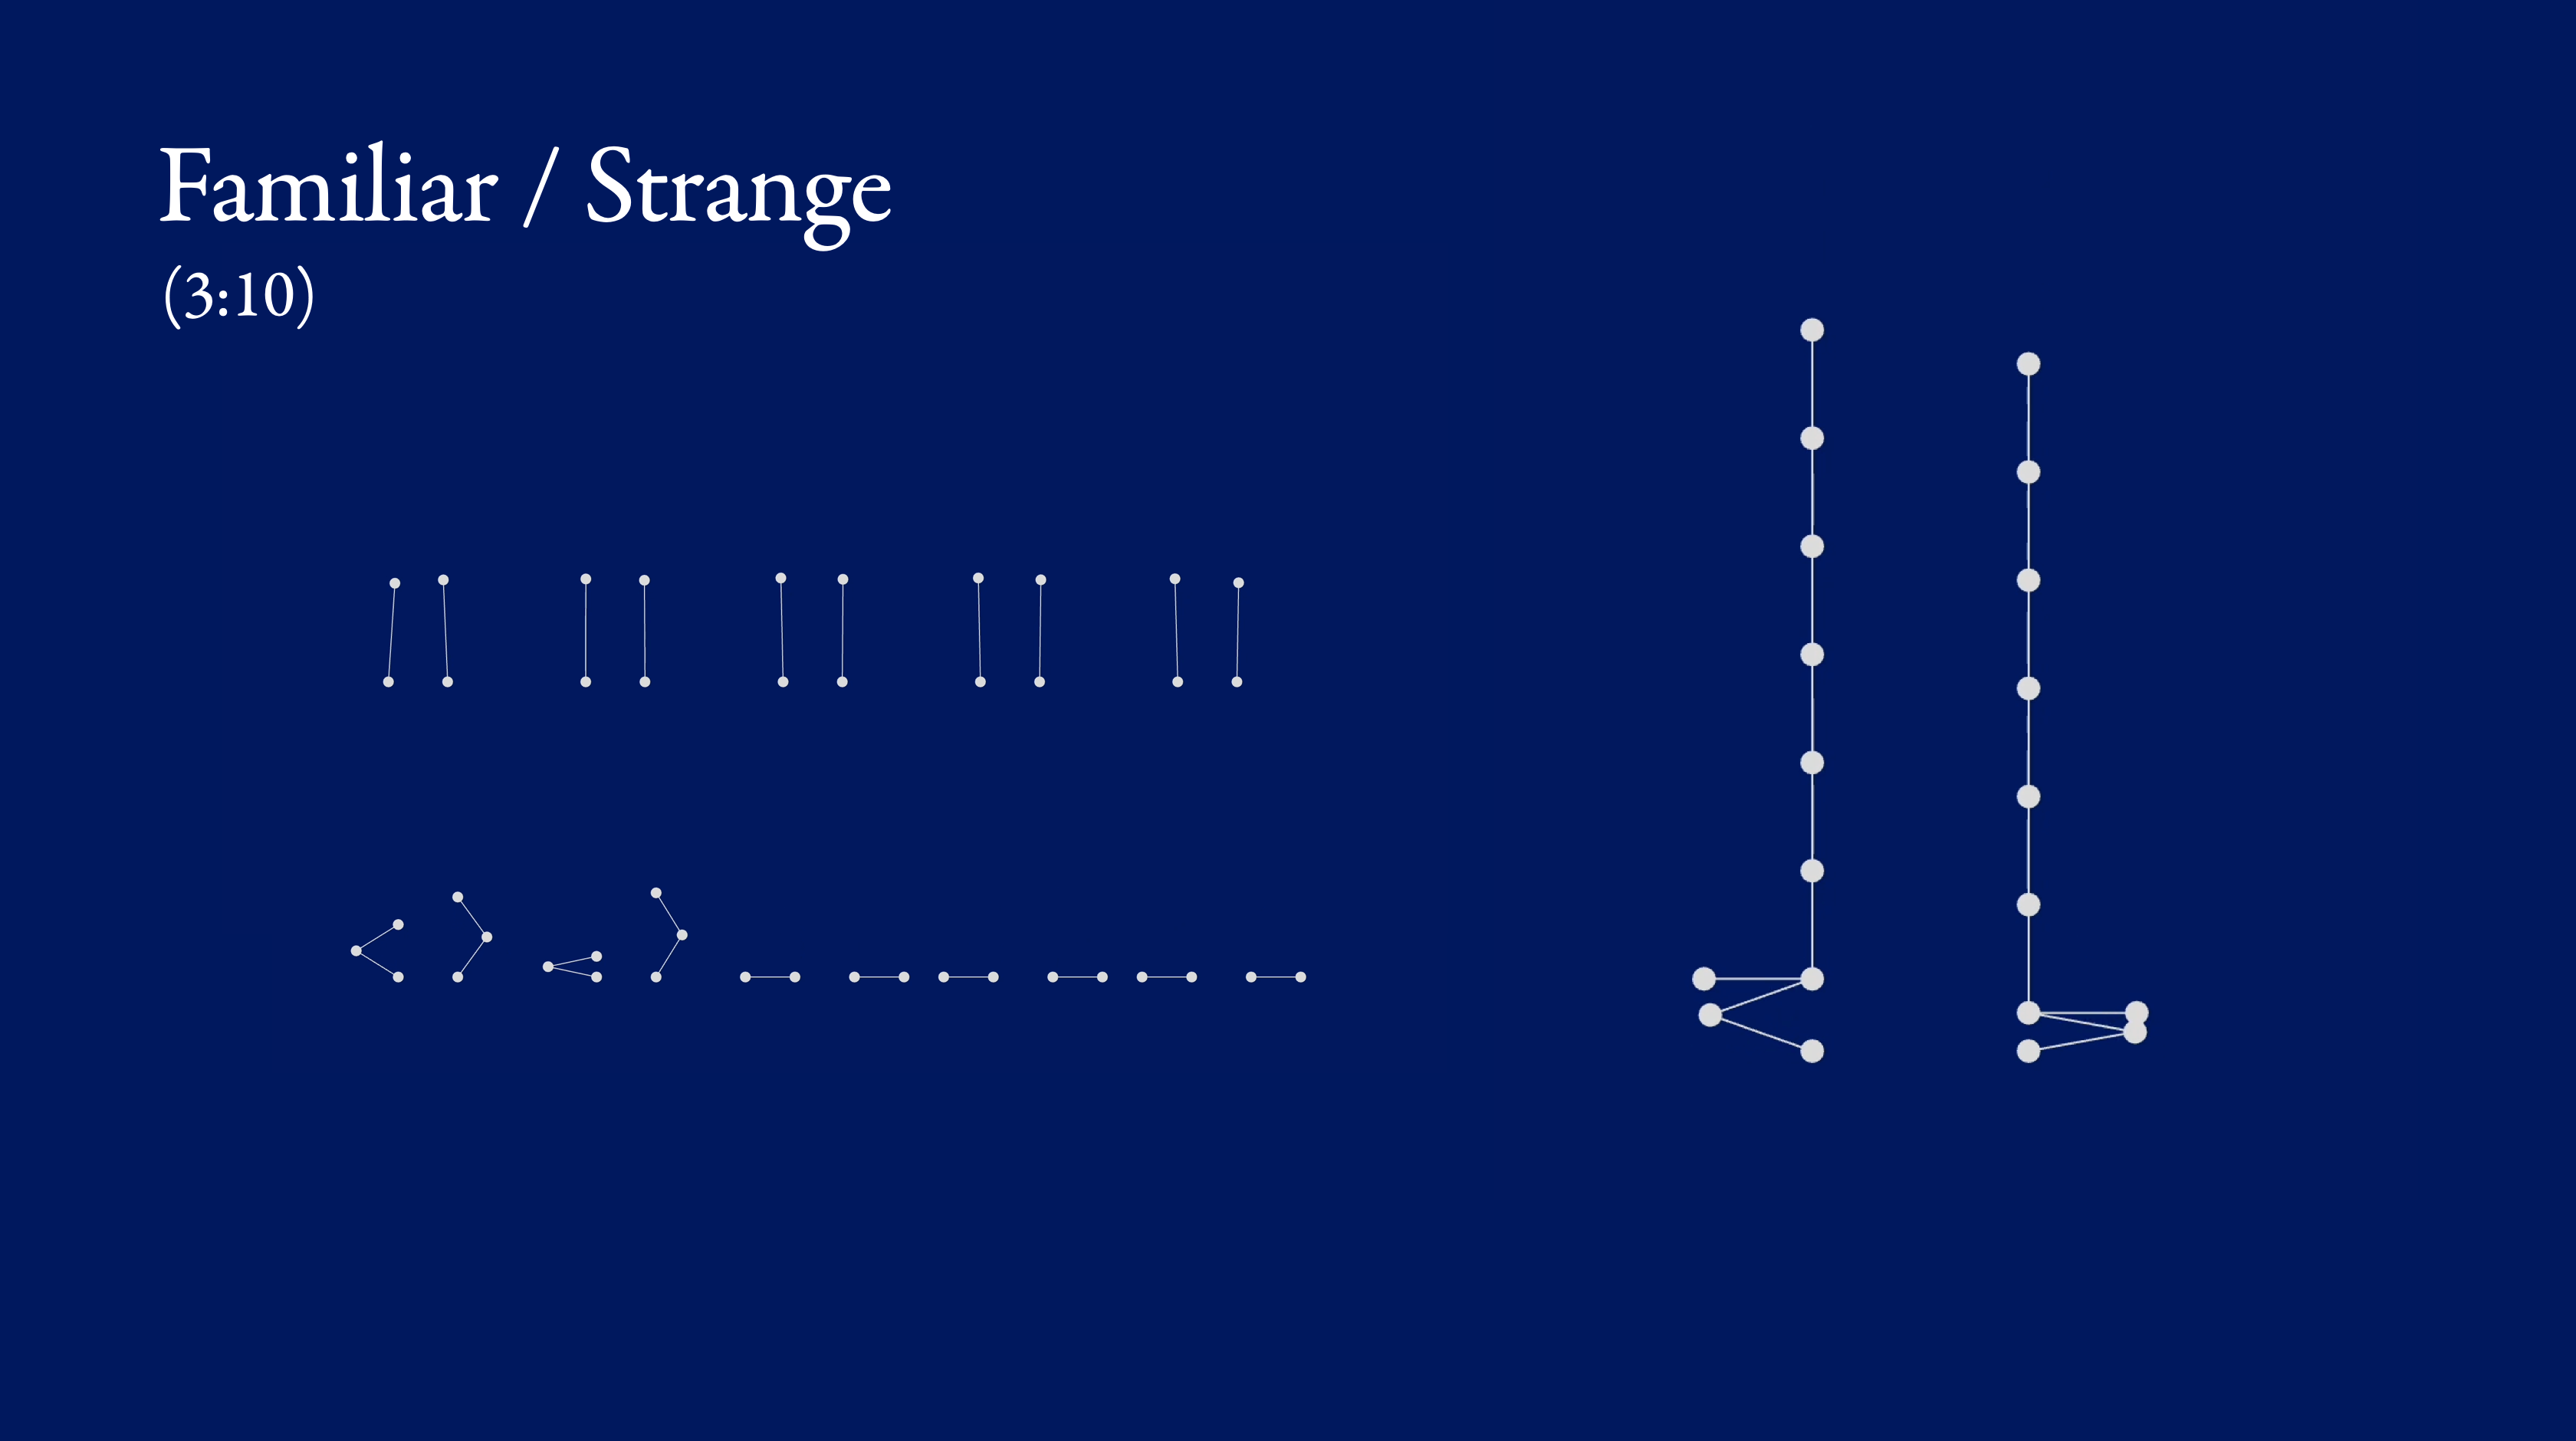
\includegraphics[width=15cm]{img/fs-02.png}
  \caption{Familiar / Strange}
  \label{fig:familiar_strange}
\end{figure}
「Familiar / Strange」は、手指の配置や関節の数・位置が次々と変化していく作品で、手の運動に対する再注目が起きることを目指している。作品は最初、手の形がそのまま現れた状態から開始し、指の並びや関節の配置の変化が起きる。一本一本の指がくの字の形をして積み上げられる様子をピークに、逆順に変化が巻き戻され、再び元の手の形に戻るという、3分10秒で1ループの構造となっている。変換の過程は、イージングやゴム紐が切れた時のような振動を伴う動きによって補完される。シーン遷移を説明する図を以下に示す。

\subsection*{Relation}
\begin{figure}[H]
  \centering
  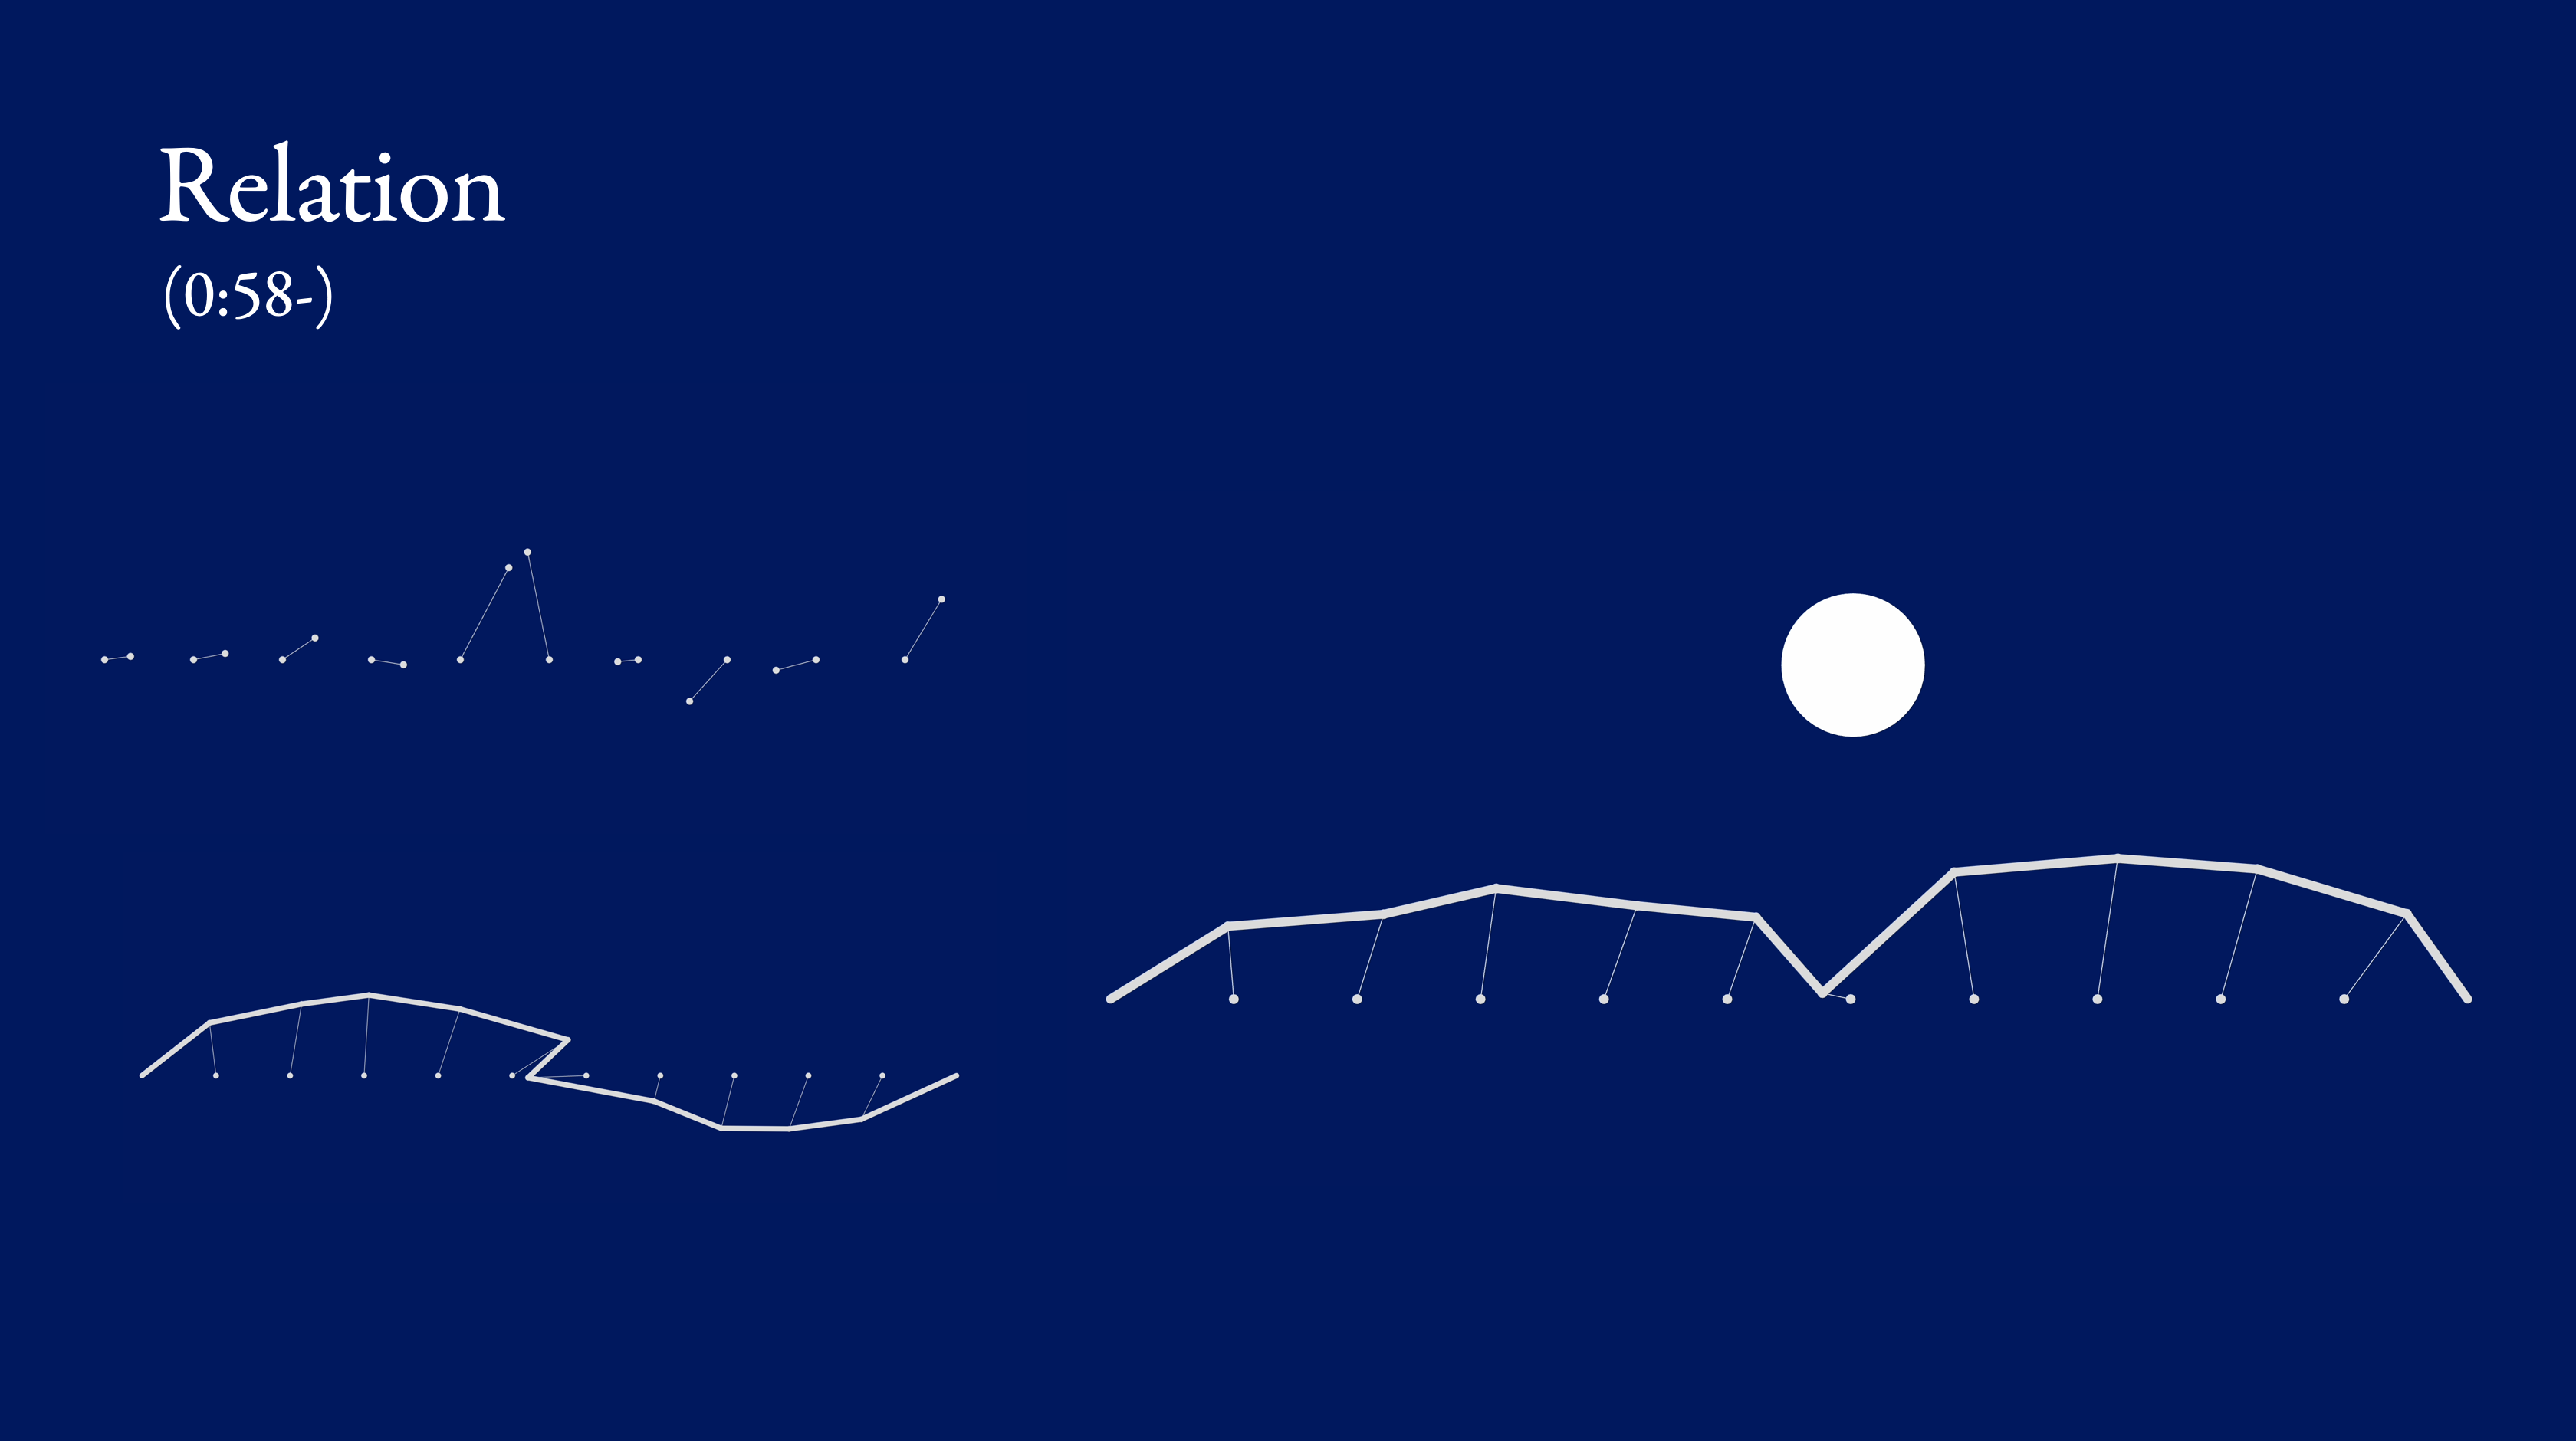
\includegraphics[width=15cm]{img/relation.png}
  \caption{Relation}
  \label{fig:relation}
\end{figure}
「Relation」は、変化した手指を取り巻く関係が次々と変化していく作品で、手と直接的に制御できないボールの関係に焦点を当てている。1つ目の作品と同様、最初は手が表示された状態から始まり、段階的に並び替えられた手指を覆う皮膜が現れ、ボールが現れる。最後はマトが現れ、的を取るたびにボールの大きさが小さくなり、3つ連続してマトにあたったとき、皮膜は消え、再び元の手の形に戻る。

トラッキングされた手指の位置が、手首から指ごとに分割され、左端から右へ、左手の小指から親指、そして右手の親指から小指の順に整列される。しばらくすると、指先以外の運動が捨象され、残された指先を結ぶ線が現れる。ここで、現れた線によって再び全ての指が1つのまとまりとして統合されることになるが、その線は後に現れるボールに対して衝突判定が適用される、新しい構造の手指を覆う皮膜のような機能を有する。皮膜のある領域を外れるとボールは落下するが、そのあとは再び画面の中央にボールが出現する。

さらに一定時間が経過すると、皮膜の上方に白い点:マトが現れる。マトに対してボールを当てると、ボールは一回り小さくなり、ボールを落とさずに合計3回マトに当てることでボールは消失し、皮膜が現れるときと逆の順序を辿って画面の中の手は再びもとの形状に戻る。

\section{作品体験のねらい}
\label{nerai}
本作について、Felsのカテゴリをもとに作品体験のねらいを説明する。

\subsection*{Familiar / Strange}
この作品におけるねらいは、トランジションの際の違和感が起点となって意識的な試行が引き出され、身体動作が変化することで一体感が生起することである。以下の説明では、便宜上図\ref{fig:diagram_familiar_strange}のように、それぞれのシーンに対して番号を割り当てる。その上で、図\ref{fig:nerai_fs}に、本作品におけるねらいを図示した(数字はシーン番号)。

\begin{figure}[H]
  \centering
  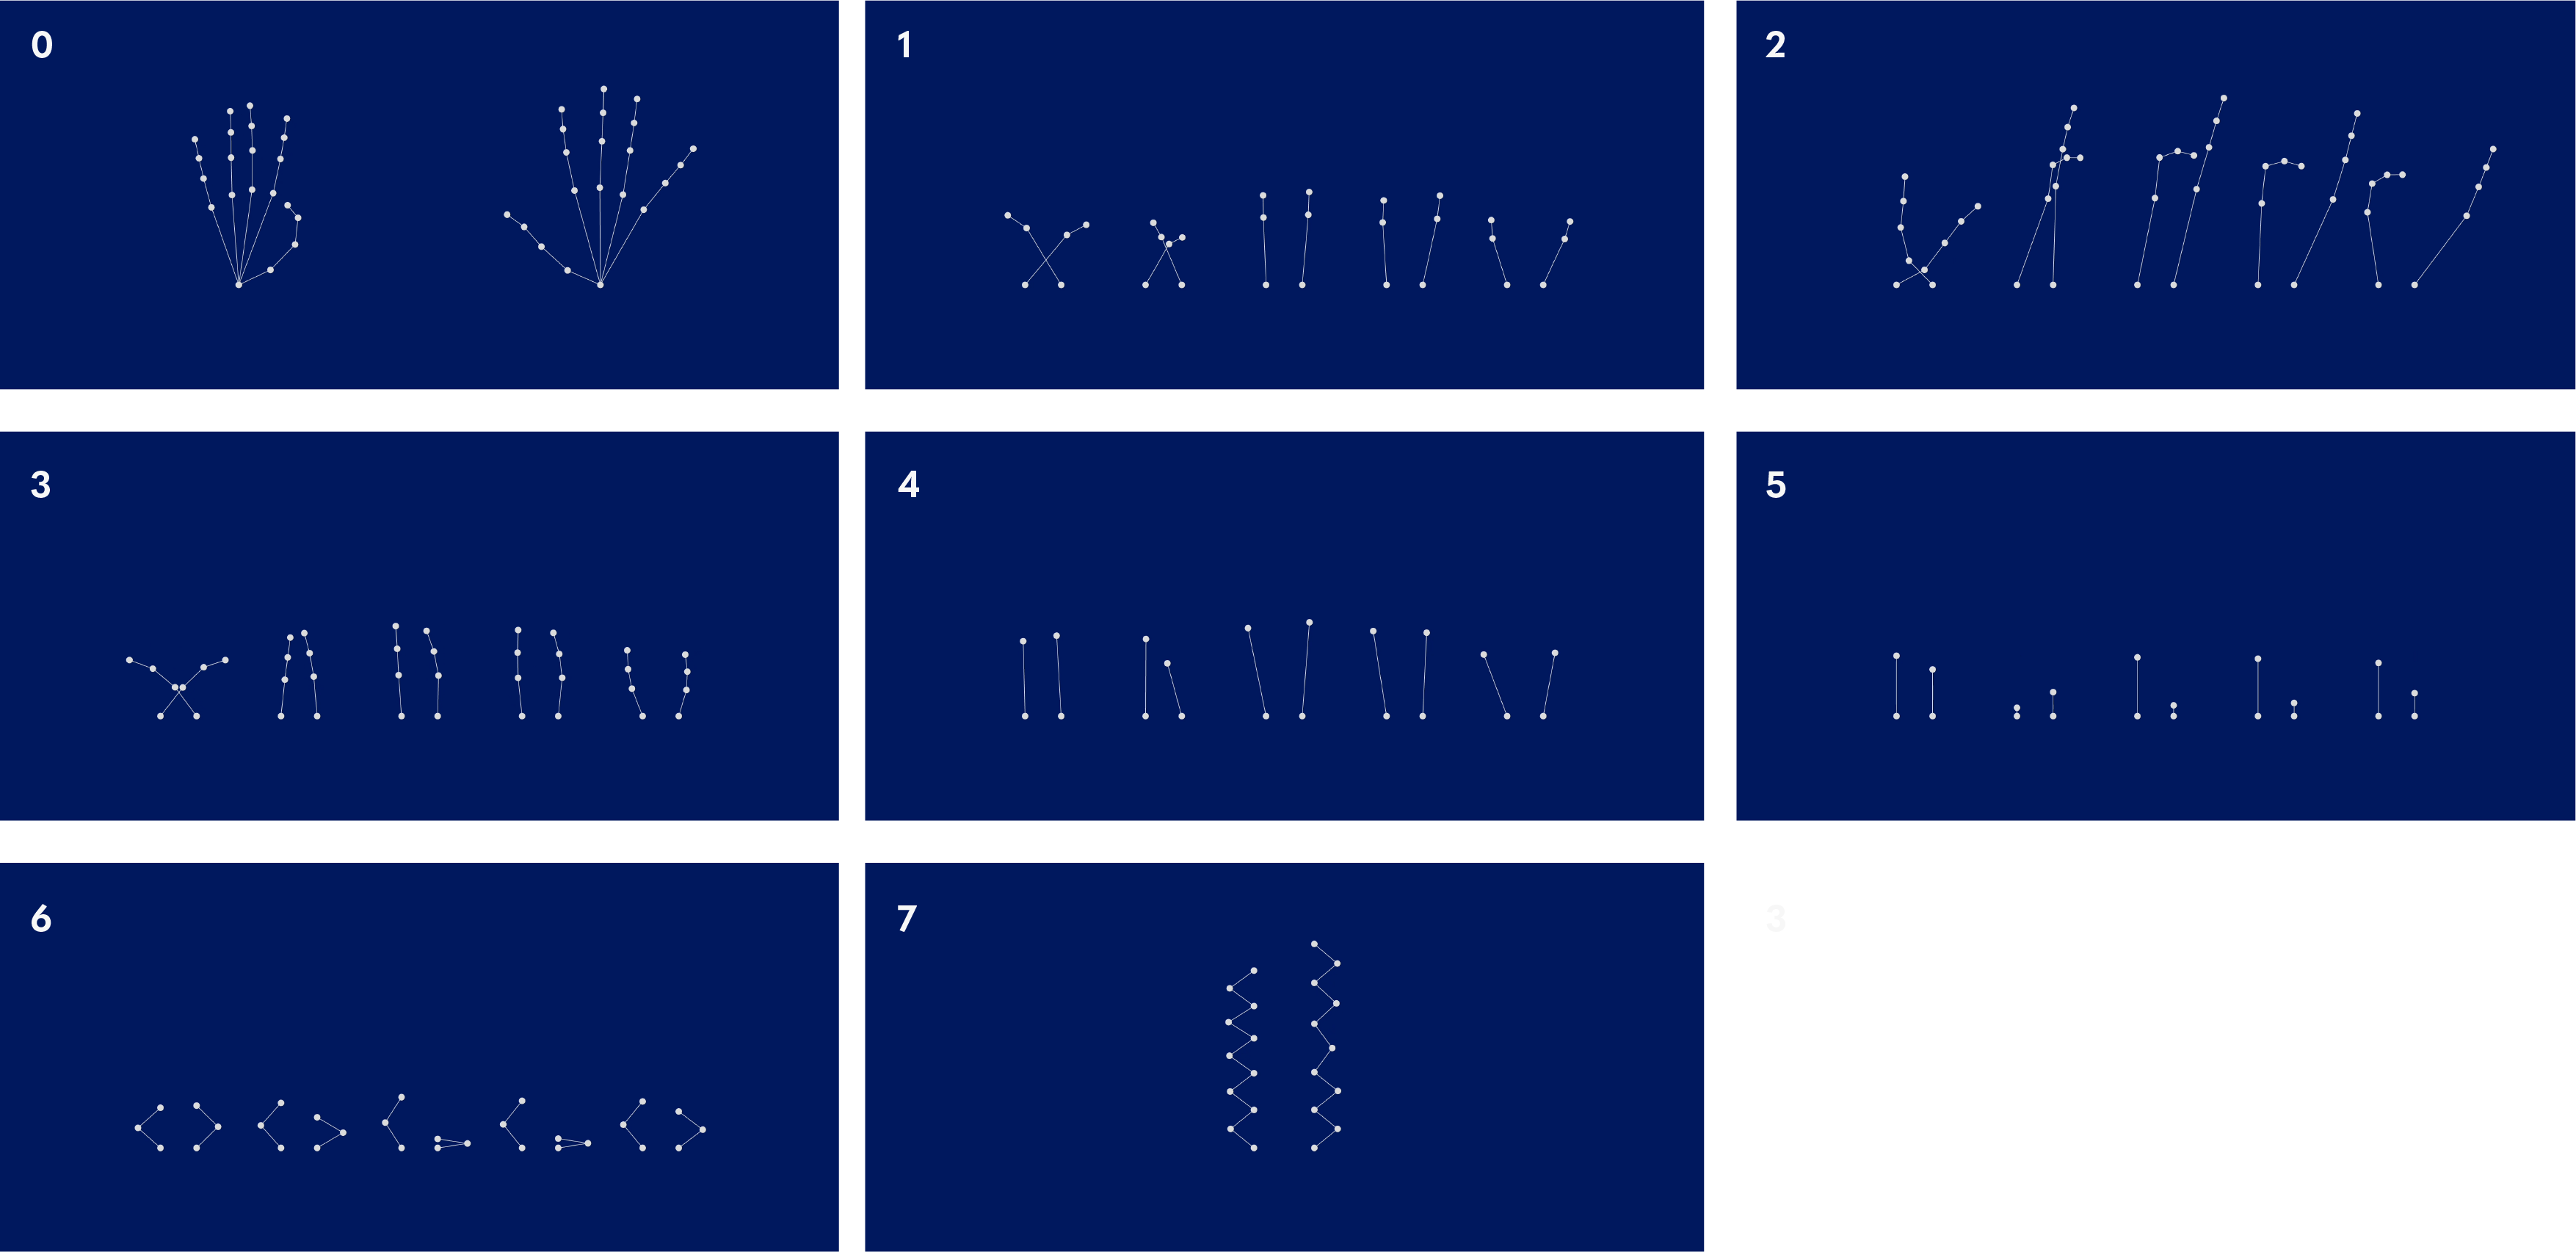
\includegraphics[width=15cm]{img/handpose-sequence.png}
  \caption{Familiar / Strangeにおけるシーン遷移}
  \label{fig:diagram_familiar_strange}
\end{figure}

\begin{figure}[H]
  \centering
  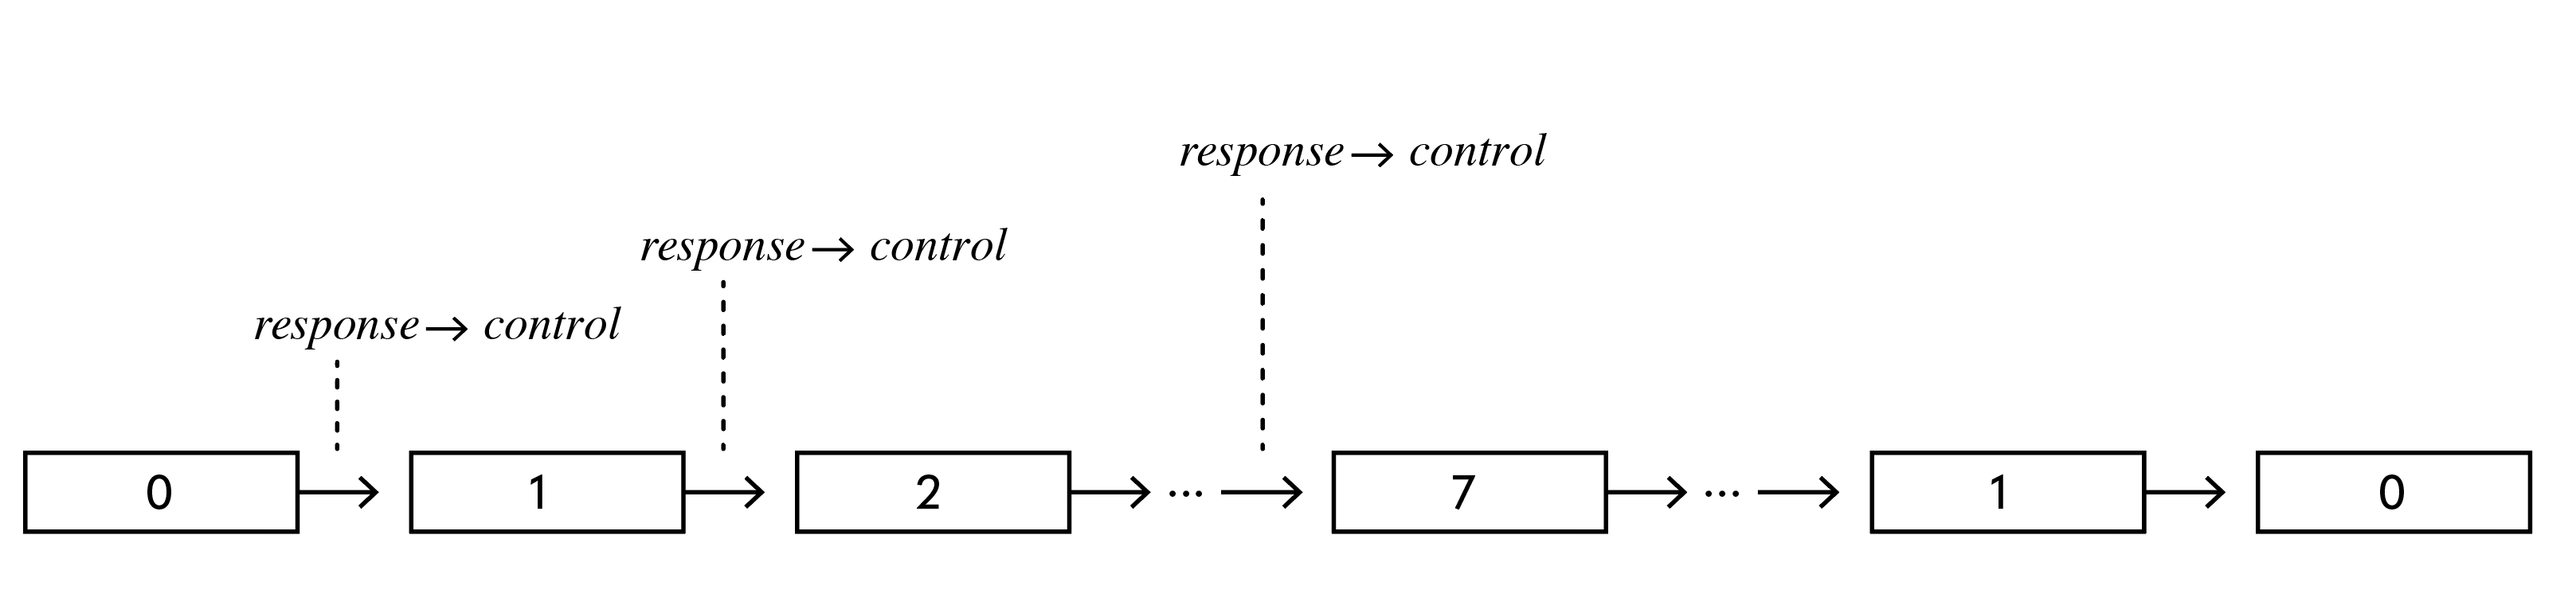
\includegraphics[width=15cm]{img/nerai_fs.png}
  \caption{《Familiar / Strange》のねらい}
  \label{fig:nerai_fs}
\end{figure}

最初、手指が鏡合わせのように表示された状態から始まり、ゆっくりと指一本一本の単位で分割されていく(シーン0からシーン1)。その瞬間に、見慣れていたはずの手指の動きが見慣れないものに感じられ、実際の手指と画面の手指との関係が、Felsの\textit{response}や\textit{contemplation}といった関係性に変化する。2つ目の作品と比べると、ゆっくりとしたテンポで手指の形状が変化する。そのためしばらくすると変化した手指の構造での身体動作を見出し、身体の動かし方が変化することで\textit{control}ができるようになると考えた。またそれが別の形に変化していくと再び関係性が変化し、その都度、構造に合わせて手指の動かし方が変化していくのではないかと考えた。また、バネ状に指の動きが連結されたとき(シーン7)には、はじめて指の動きが相互に干渉するようになり複雑度が増す。そのため、ある形や運動を持続させるためには複数の指の連携をとる必要が生じるため、それができるようになることでより強い一体感(\textit{intimacy})を感じるのではないかと考えた。

\subsection*{Relation}
この作品におけるねらいは、ボールの操作やマトに当てるといった目的意識が起点となって意識的な試行が引き出され、その目的を達成するための技量を身につけることで一体感が生起することである(図\ref{fig:nerai_rl})。ボールは手指のように直接動かすことができないため、目的意識が生じてもそれを即座に達成することができない。身体の動かし方を画面内の構造にあわせて変化させるだけでなく、ボールの動きを制御するための、より緻密な運動の統合が求められる。このようにして、巧みさを獲得することでボールが思い通りに動かせるようになる(\textit{control})ことで、一体感(\textit{intimacy})を感じるのではないかと考えた。またこの作品では、手そのもの、手とボール、ボールとマト、というように、段階的に緻密な運動の制御が求められることで、一体感(\textit{intimacy})が高まるのではないかと考えた。
% ボールと手の関係に注意が向いた途端、手指に感じる違和感や注意は向きづらくなる。さらに、マトが現れると、さらにその目的意識は強固になると考えた。これまでの展示の様子から、ボールと手指だけの関係性であっても、まずは飛ばしてみる、転がしてみる、落とさないように気を付けるといった目的意識を設定しやすい。その一方で、手指のみの状態から手指とボールとの関係性に切り替わったときと同様に、マトが出現することがそうした注意を不可視にしてしまうことがこれまでの展示の中で見受けられた。

% そのため、手指の変換、皮膜の出現、ボールの出現、そしてマトの出現は、それぞれタイミングを分けて出力するように調整した。本作はダイナミックな構造の切り替わりこそ少ないが、手指を取り巻く関係性が次々に変化する作品として構成された。そうすることで、それぞれの関係性において異なる注意が生じ、段階的に目的意識が強固になっていくことで、「マトにボールを当てる」という強い目的意識とその達成のための試行錯誤を通して、強い一体感が生じるのではないかと考えた。

\begin{figure}[H]
  \centering
  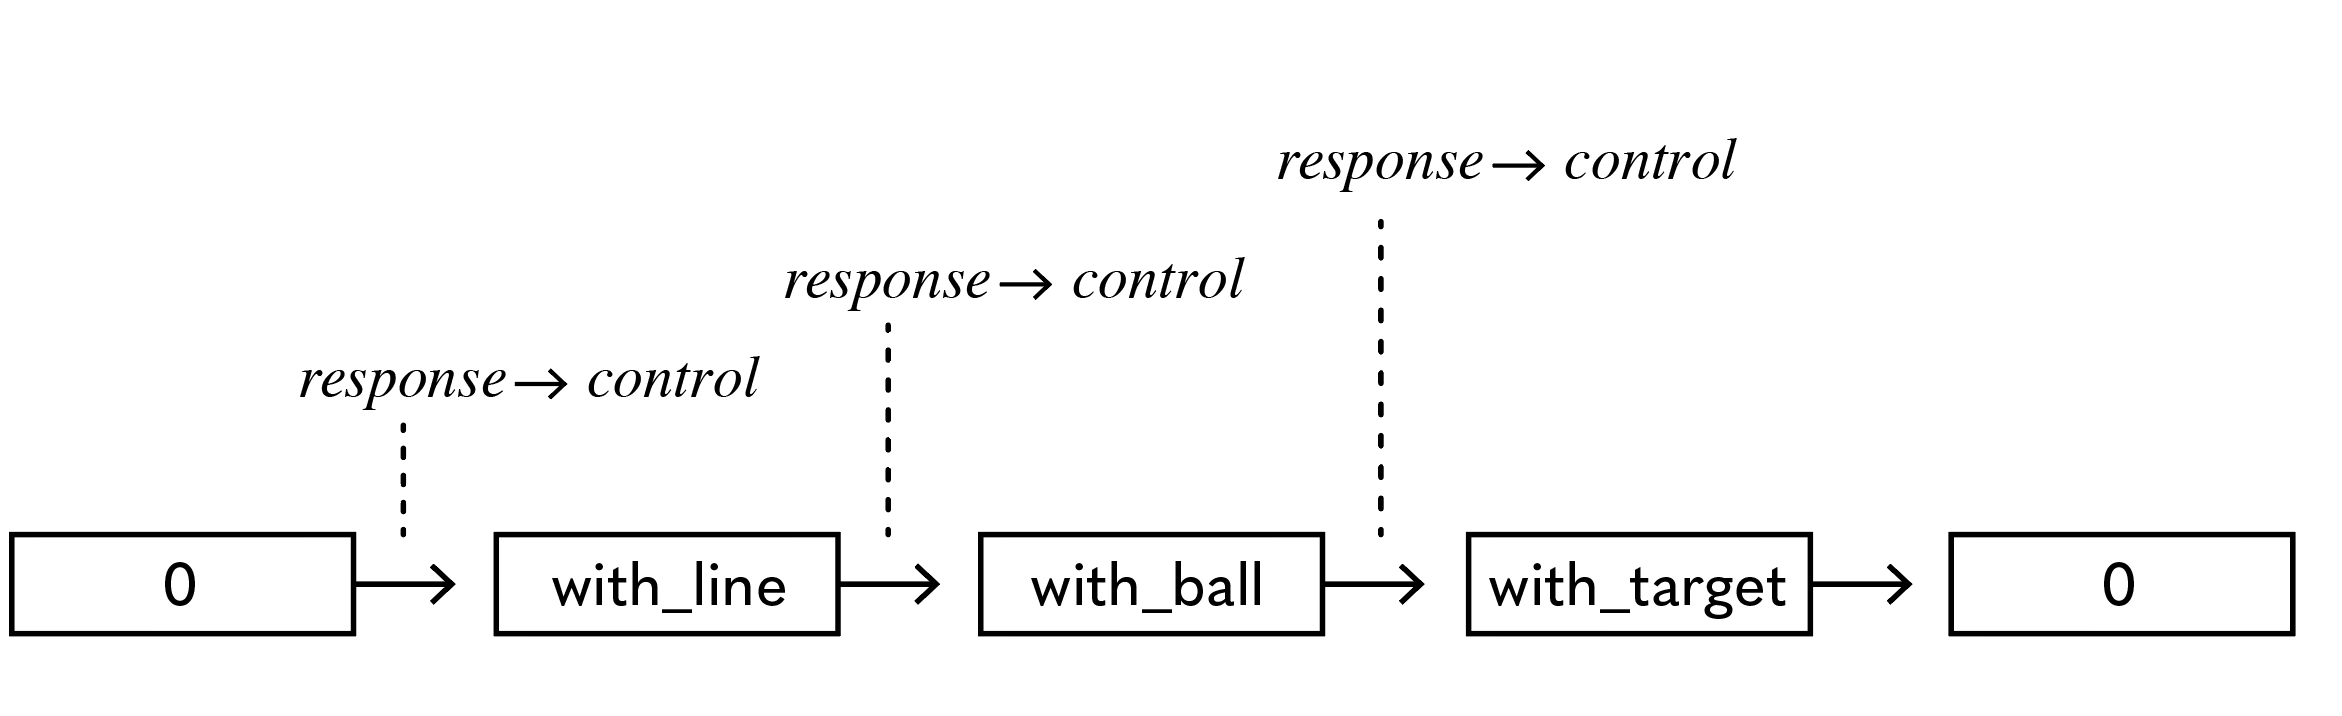
\includegraphics[width=15cm]{img/nerai_rl.png}
  \caption{《Relation》のねらい}
  \label{fig:nerai_rl}
\end{figure}

% \textit{grasp}には二つの性質がある。一つは、時間幅が注意を向けている対象によって、長い場合と短い場合があることである。目的意識が芽生えてからスムーズに操作できるようになる場合、'reach'から'manipulate'が近く、\textit{grasp}は短い、すなわち直感的で使いやすいものとして経験される。その一方、目的意識が芽生えてから試行錯誤を伴い、習熟に長い期間を要する場合、\textit{grasp}は長く、もどかしさを経験し、操れるようになった時に達成感を経験する。\\

% 二つ目に、\textit{grasp}の過程で他のことに対する意識が次々と芽生えることがある。具体的には「やってみるまでわからない」といった経験や、物事に対する解像度が高まる中で、当初とは異なる意識が芽生える状況に相当する。\\

% このコンセプトを展開し、「試行錯誤の余地」を設計することを目指したのが、修士作品《Grasp(er)》である。この作品では、\textit{grasp}を経験する中で、個人による創造的な活動が生まれ、\textit{grasp}という動作を行っているのではなく、そこに'er'の接尾辞がついた'Grasper'であると名付けた。
\newpage

%----------------------------------------------------------------------
% 5章 結論
%----------------------------------------------------------------------
\chapter{バリデーション}
\label{validation}
\section{概要}
制作された修士作品が実際にはどのように体験されるのかについて調査した。

\section{実施方法}
\subsection{Video Cued-Recall メソッド}
本作品を評価する上では、体験時、体験者がどのようなことに注意を向け、どのような行動を取ったかについて精緻に振り返る必要がある。そのため本研究では、Video Cued-Recallというメソッドを用いて体験時の言語データの収集を行なった。 Video Cued-Recallとは、体験時のようすが記録された映像を視聴しながら、体験者本人が映像を手がかりに作品での体験を回顧し、言語化する方法である\cite{Costello2005}。インタビューを通して回顧するよりも詳細に体験を振り返ることができ、また体験しているそのときに体験のようすについて語ってもらう方法よりも、自然な体験について記述できることがその利点として挙げられる。

\subsection{参加者について}
インタビューは、FabCafe Nagoyaでの展示に際して、4名の体験者を対象に実施した。ただし、うち1名(参加者4)は「Relation」の体験時、トラッキングの精度が著しく低下していたため、1つ目に体験した「Familiar / Strange」の体験についてのみ調査の対象とした。

\begin{figure}[H]
  \centering
  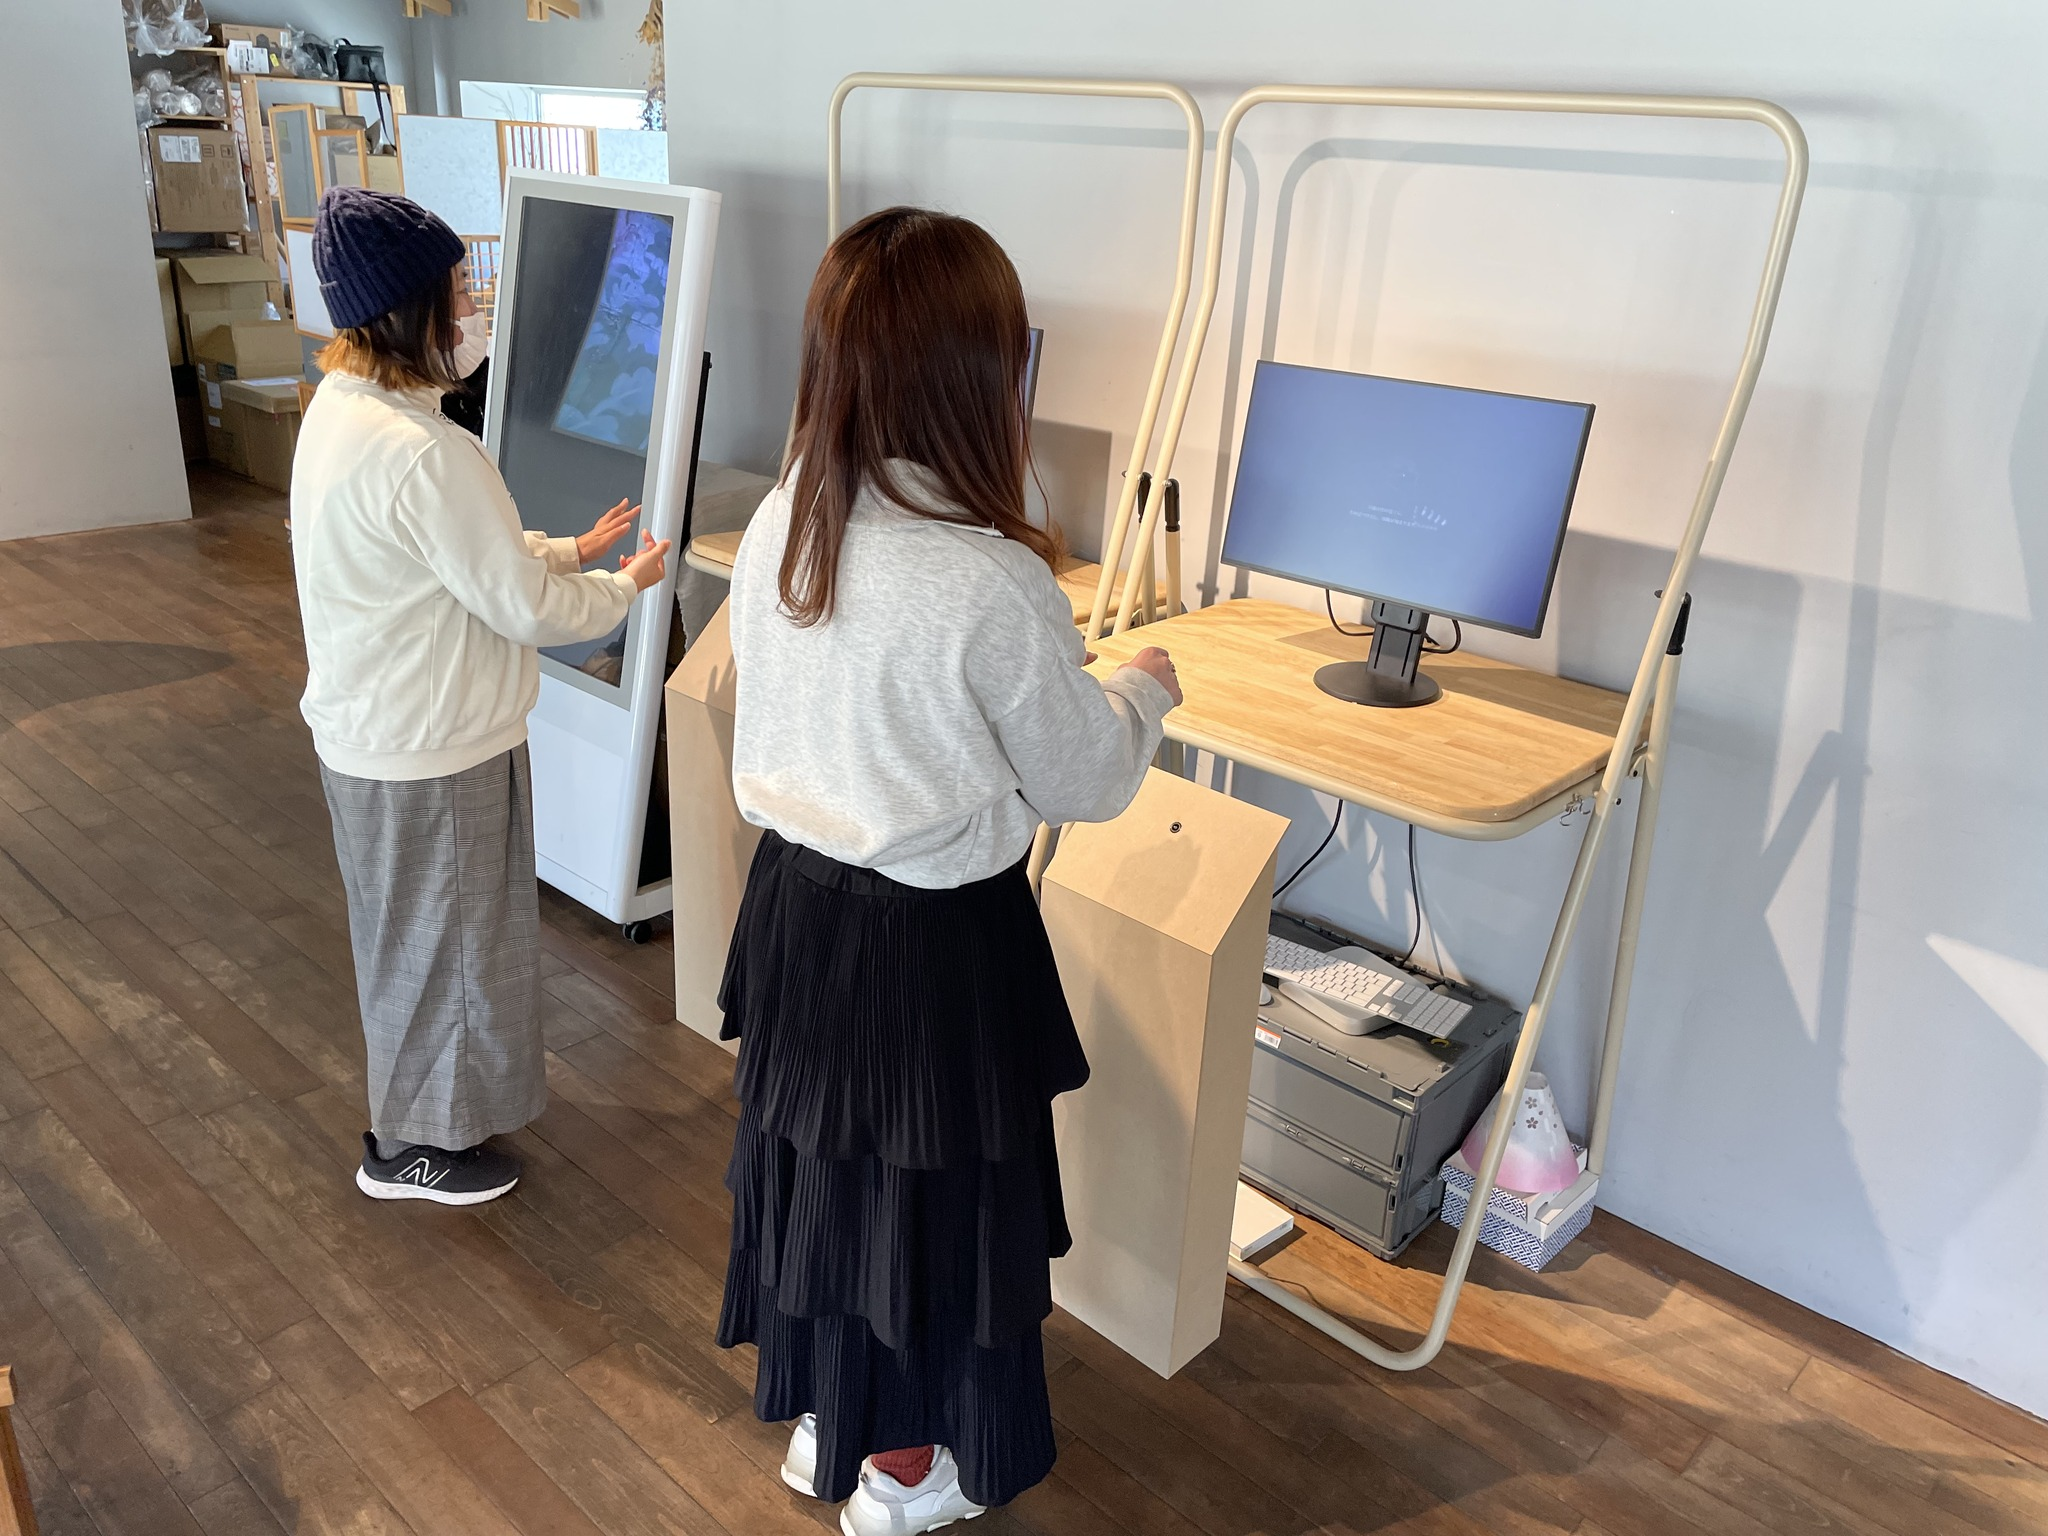
\includegraphics[width=10cm]{img/exhibit_at_fabcafe.jpeg}
  \caption{FabCafe Nagoyaでの展示}
  \label{fig:exhibit_at_fabcafe}
\end{figure}

\subsection{データ収集}
参加者にはまず、調査の大まかな流れについて説明し、撮影についての許諾を得た。コンセプトの説明が自然な体験に影響することを避けるため、作品の体験の前にはコンセプトや具体的な作品の内容については説明せず、トラッキングされた手が次々に形を変えていくこと、手の形が表示された状態から始まり、再びもとの手の形に戻るループ構造のある作品であること、という最低限の構造のみ伝えた。

体験のようすは、手もとのハンドトラッキングを行うカメラ映像、現在時刻、体験者が実際に見ているスクリーンの映像が図\ref{fig:record_monitor}のようにレイアウトされて記録される。

\begin{figure}[H]
  \centering
  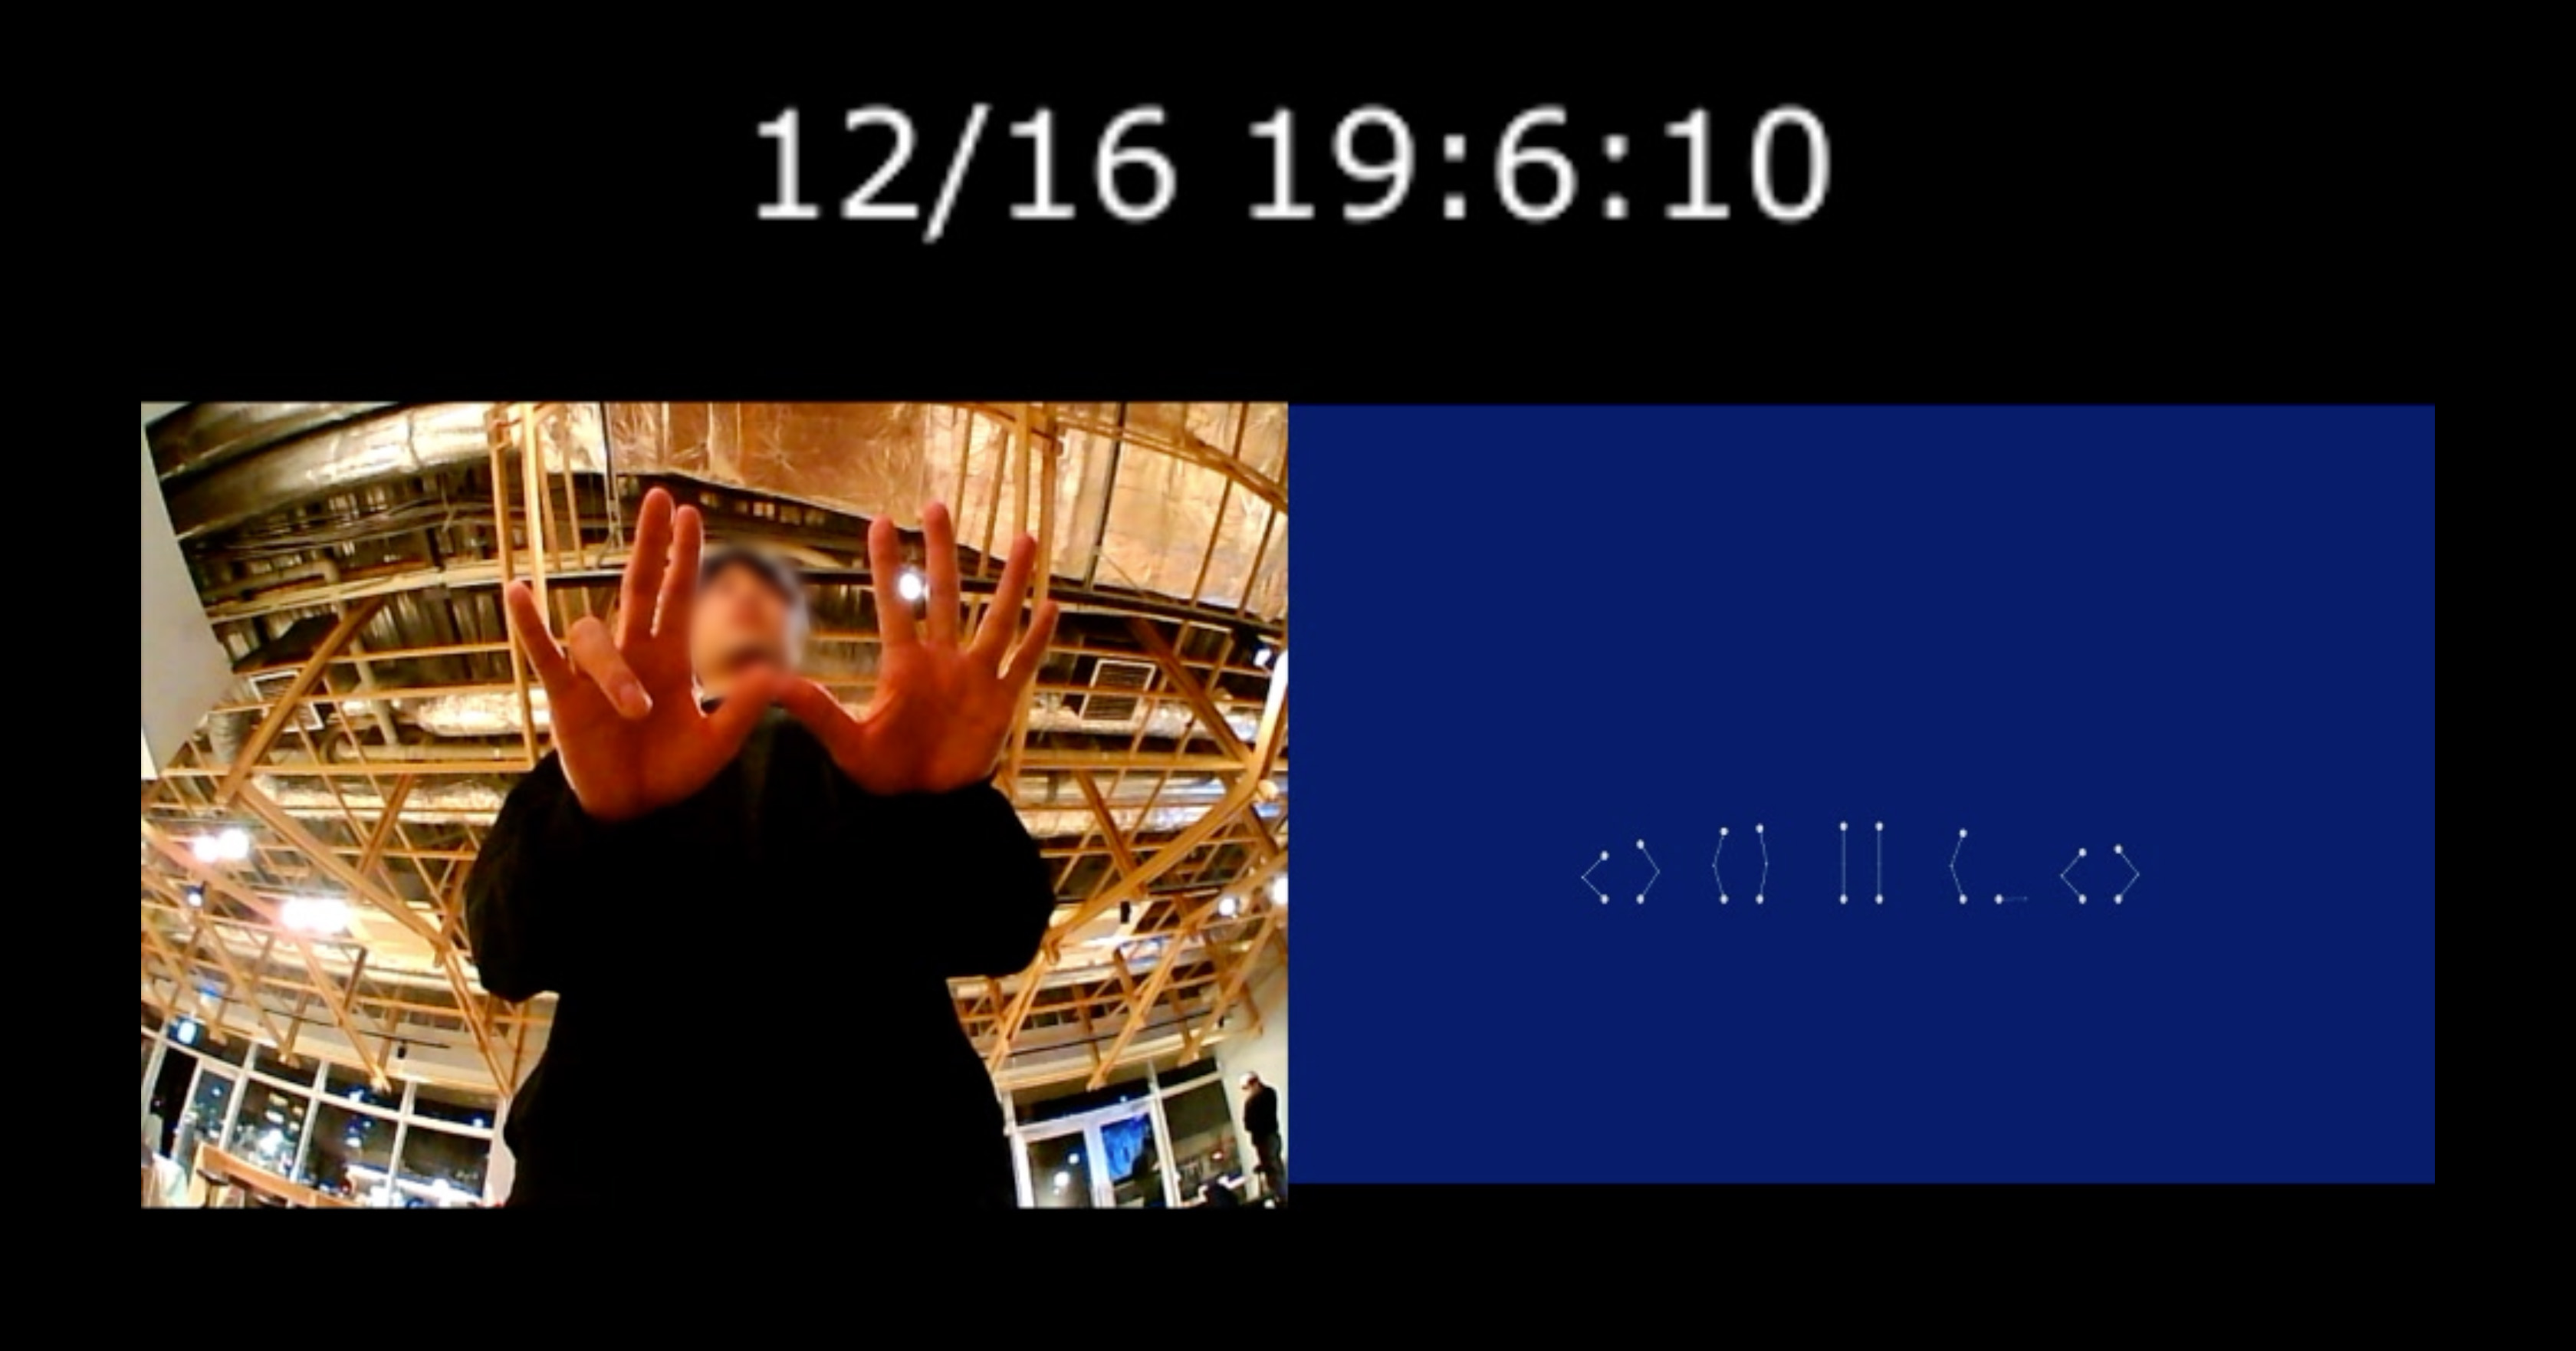
\includegraphics[width=10cm]{img/record_monitor.jpg}
  \caption{体験のようすの記録映像}
  \label{fig:record_monitor}
\end{figure}

作品体験が終了した後、体験者自身が上記の記録映像を視聴しながら、作品体験時のようすを詳細に言語化する振り返り作業を依頼する。この時点では、そのとき考えていたことや、試行した事柄とその理由など、作品体験を終えた今思う感想ではなく、その当時経験していたことについて言語化してもらうよう促した。体験者は、自由に映像を停止したり、巻き戻すことができる。
作業の際は研究実施者も同席しているが、調査を実施する上でのトラブルが生じない限り、原則体験者個人で振り返る。\\
その後、前の振り返りの作業や体験のようすを踏まえて、研究実施者が半構造化インタビューを実施することで、より精緻に作品体験のようすを振り返るとともに、体験を終えた上での感想などについて伺った。
いずれもループ構造の作品であるため、1周するまでの期間をその調査対象とした。ただし、作品「Relation」については、一周するための達成条件がシビアであることから、体験の終了は3分以上体験することを目安に、いつでも体験を終了してよいこととした。

\subsection{データの記録}
インタビューから言語化された体験時の回想を、図\ref{fig:spreadsheet}のようにスプレッドシート上に時系列で記録した。シート上には、1秒ごとのタイムスタンプ(日本標準時)、その時刻でのトラッキングの状況(右手、左手、全体)、その時刻での出力内容を示すシーン情報、並びに発言内容が記録されている。また、その後に行ったインタビューについては文字起こしをしてテキストデータで記録した。
\begin{figure}[H]
  \centering
  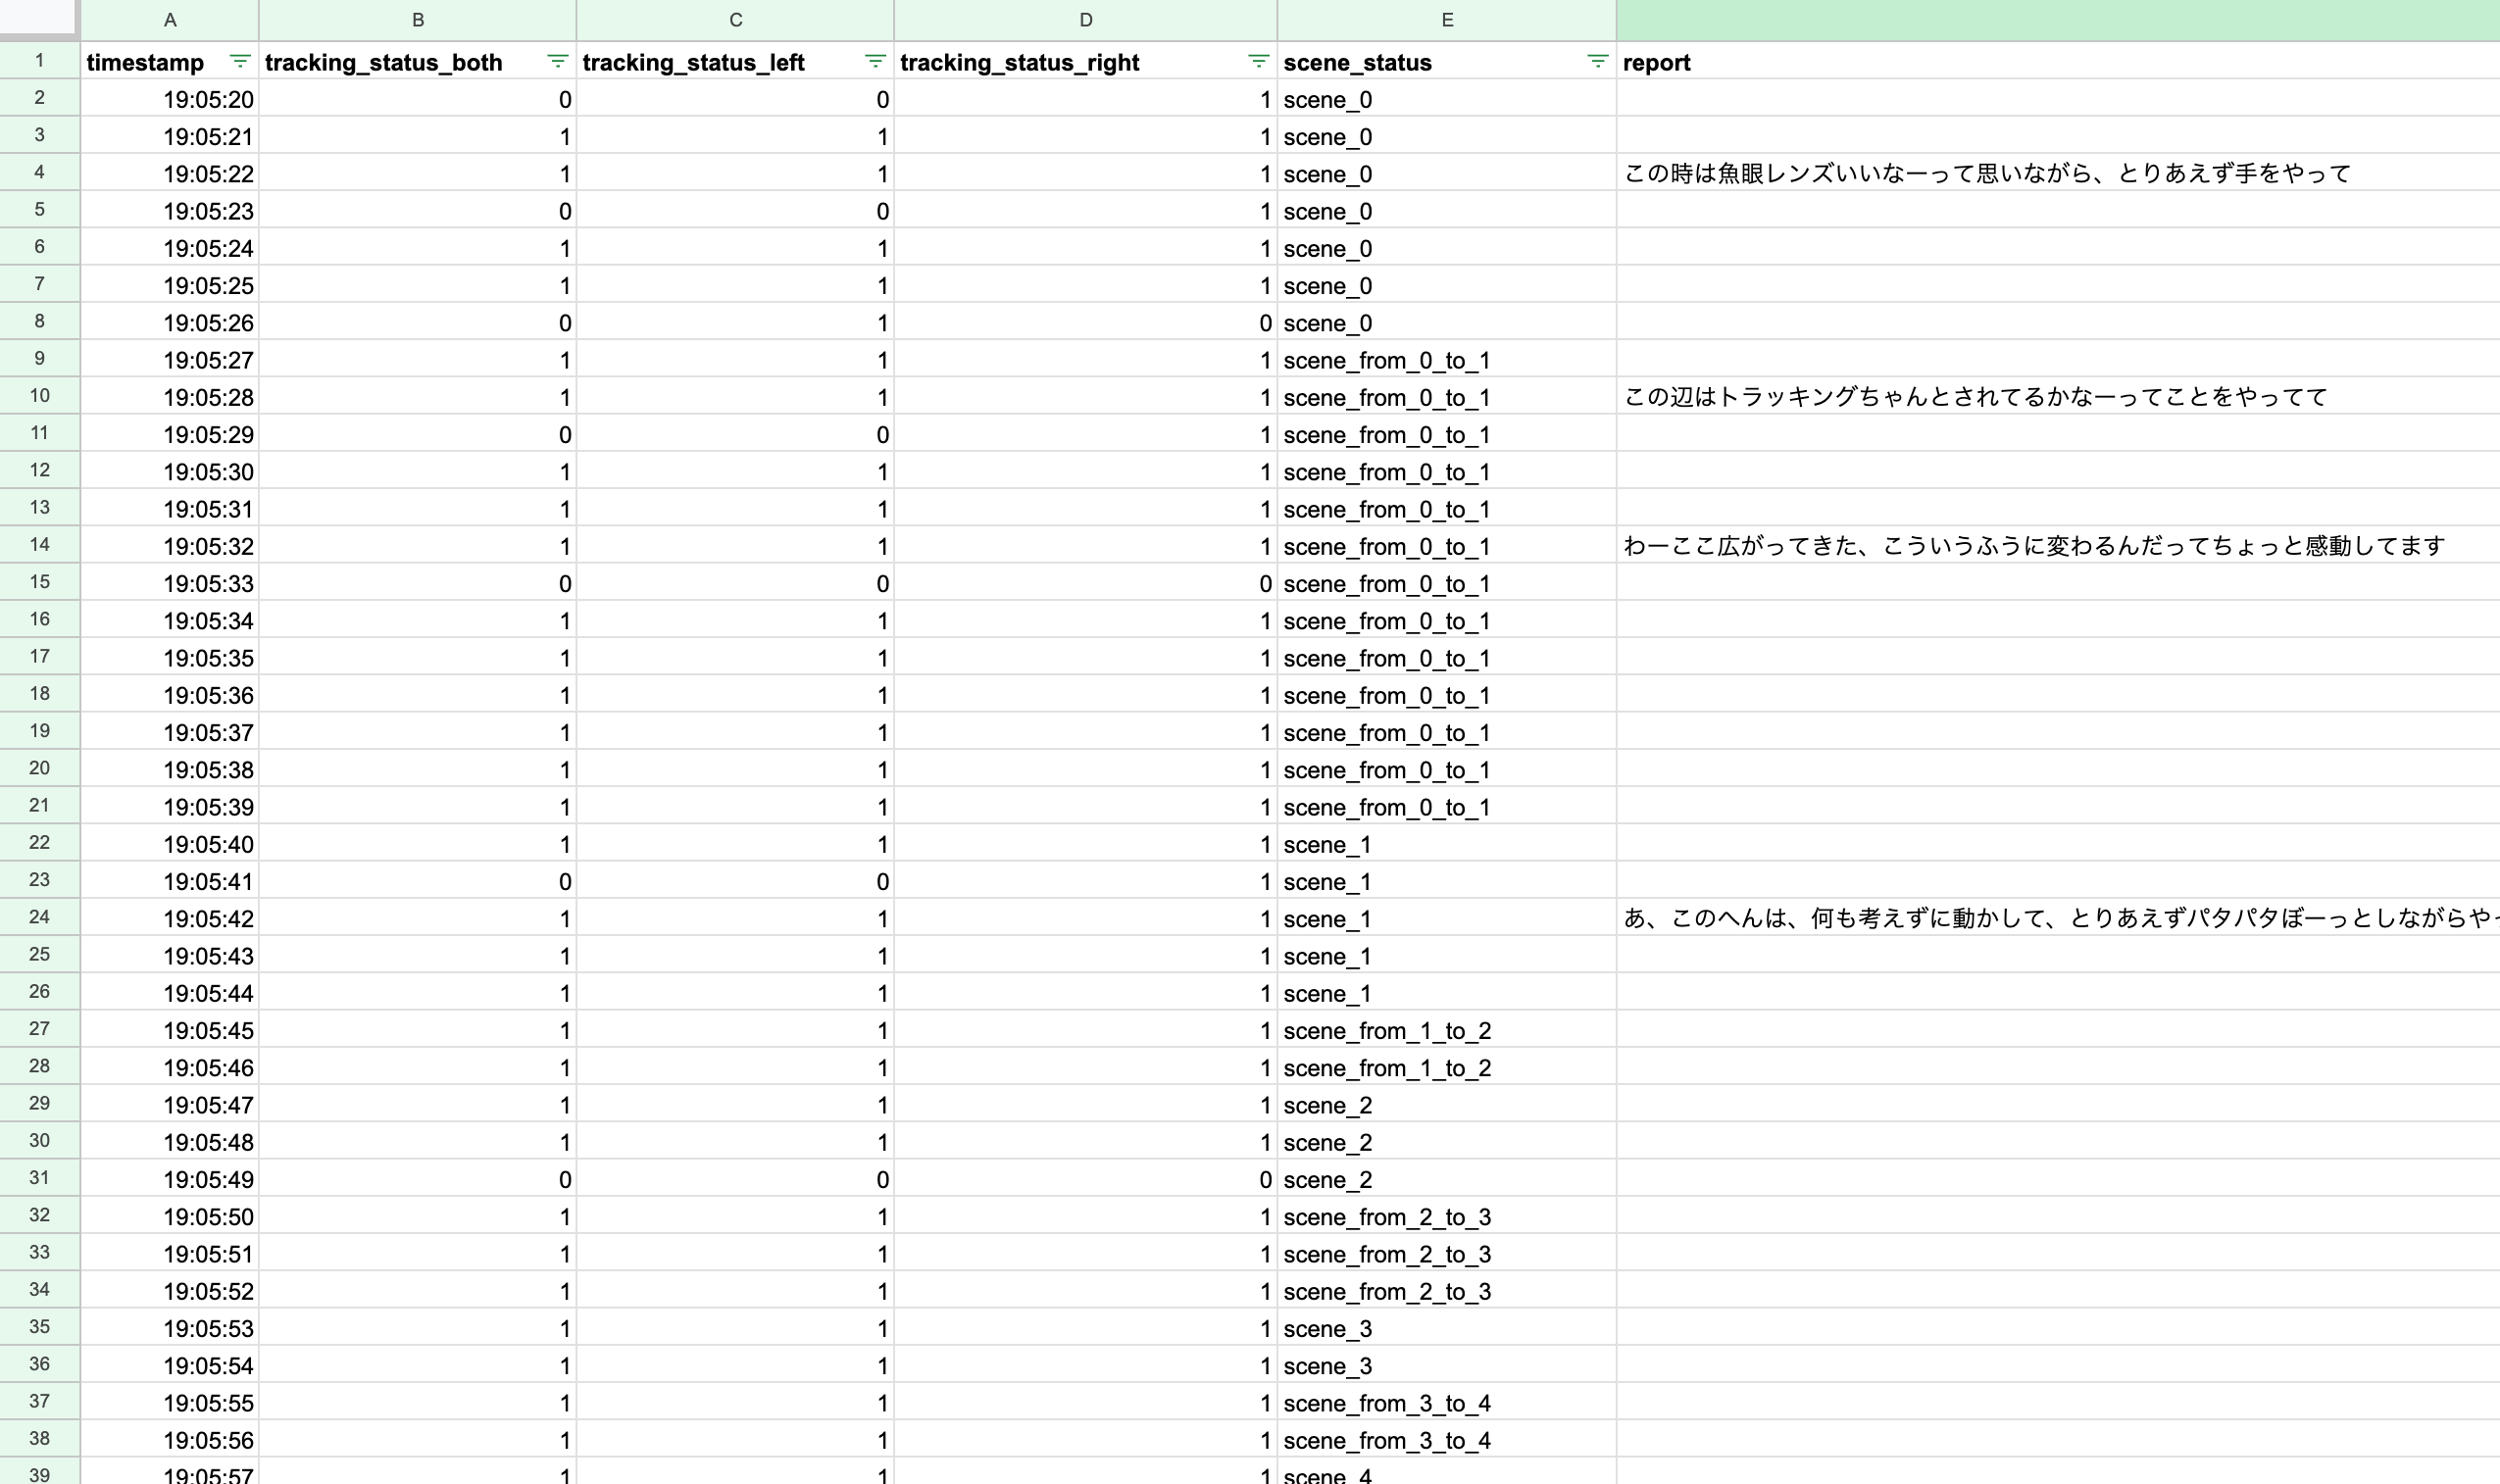
\includegraphics[width=10cm]{img/spreadsheet.png}
  \caption{発話情報が記録されたスプレッドシート}
  \label{fig:spreadsheet}
\end{figure}

\section{結果}
以下では、参加者の体験時の映像とそれをみながら体験者自身が行った回想、そして、インタビューを通して得られた意見から、それぞれの参加者が「Familiar / Strange」、「Relation」をそれぞれどのように体験していたのかについて説明する。

\subsection{Familiar / Strange}
\subsubsection*{参加者1}
参加者1の手指の動きをみると、scene0からscene1にかけての、手が指ごとに離れていく過程では、手を握りしめたり、開いたりする動作が見られるが、scene1以降、関節が減り、左右の指で1セットのまとまりが明確になってくると、指を一本一本曲げる動きをするように変化した。手指の単位で分かれる「Scene1」から「Scene6」にかけては、どの指がどの指に対応しているのかについての「確認」を主に行なっていたと語る。
\begin{quote}
  どれがどの場所なんだろうって、最初は手の形になっているのでわかるんだけど、それがずれていってどれがどれかなっていうのを確認してたかな。
\end{quote}
しかしscene7になると、途端に握り拳を作る動きが多くなる。また、右手と左手を交互に握ったり、指一本単位でも、左右で同じ位置の指を曲げる動きが現れる。体験を振り返って、「干渉するイメージが強くなった」ことについて語る。
\begin{quote}
  今まで二つ単位で独立してたのが全部つながってバネみたいになって、お互いがお互いに干渉するイメージが強くなったかな。全部握ったら、全部閉じるんだ、みたいな。
\end{quote}
そして、「干渉」構造に気づいた後のscene7以降も手指の動きに注目すると、前半には少なかった左右の同じ指を同時に動かす動きが増えた。そして最後に両手を翻して、手を裏向きにした状態でもトラッキングができているかについて確認しているようすだった。\\
\subsubsection*{参加者2}
参加者2は最初、グー、チョキ、パーといった手全体でできる形を通して、「自分の手と、モニターに写っている手が、どれぐらい親和性高く動くのか」について確かめていた。また、しばらくは手を高くあげたり、下げたり、また両手を重ねたりすることで、トラッキングができる領域や認識精度の限界について確かめていた。Scene3から4にかけては、「親和性から離れていく感じ」があると語る。
\begin{quote}
  ここら辺からちょっと違和感というか、親和性を確かめてたのに、その親和性から離れてく感じがしてた。今の自分の手と、こっち側の手の連動が、してるんだけど離れている。自分の手じゃなくなる。
\end{quote}
また、参加者2は特に、手指を高速に動かすことで、どのスピードまで反応しうるかについても確かめていた。しかしScene7では、手指を高速に上下させても反応して動いている様子から体験中に「気持ちいい」と語っていた。
\begin{quote}
  ここら辺から自分が気持ちいい動きが探っていて。細かい動きを認識するなっていうのがここら辺でわかったから。ただ大きい動きになると、センサーの反応が悪くなったから、気持ちよく動く限りで、細かい微妙な動きをしたり。
\end{quote}
その後、再び元の手の形に戻るまでの過程では、腕全体を大きく振って指揮者のような動きをしながら、「俊敏な動きに対するトラッキングの時間差」を探っていたと語る。また、指揮者のような動きをしたことについては、「目視で手を見るだけでは認識することのできないような、指揮者の手の仕草など」が、「ビジュアルで出てくるとわかりやすい」といったことを想像していたと語った。

\subsubsection*{参加者3}
参加者3は最初、フレーミングする手のジェスチャーをするなどして、形を作っていた。しばらくして、自分の動きとは関係なくシーンが遷移していることに気づくと、手を動かすことを止めて「自分が動かなくても動く」ということを確かめていた。ほかにも、「徐々に、点がなくなっていくのを見ながら楽し」むなど、手指を動かさなかったときのシーン遷移についての感想が多かった。しかしその一方で、他の参加者1、2とは異なり、指を一本一本動かし、どこがどの指であるかを確かめるような動きは少なかった。
scene3から4に遷移する過程で「こうやってしたら(両手を開いて親指と人差し指をつなげ、三角形を作る)くっつくのかな、みたいなことをやっていました。特にくっつかなかった。」「(指を交差させて)こうやってやったら変わるのかな」と、「形を作る」ことができるのかについて試行していたが、結果「作れなかった」と認識してからは、手を開いた状態で、カメラに手を近づけたり遠ざけたり、手首を回すような動きをとっていた。そして、体験については「途中で飽きていた」と振り返った。インタビューにおいてその理由を尋ねると、「反応が変わらない」ことがその理由であると語った。
\begin{quote}
  関節五個あった時は楽しかったんですよ。それが一個になって、あれ、なんか手を動かしても広げなくても変わらない、やってもやらなくても反応が変わらない。ならやらない、みたいな。  
\end{quote}

\subsubsection*{参加者4}
参加者4は最初、手指の動きが認識されたことを受けて、トラッキングがどの程度の精度で認識するのかについて確認していた。すると、scene0からscene1にかけての初めてのシーン遷移を受けて、「こういうふうに遷移するのかということに、ちょっと感動していた」と振り返った。その後、scene1に遷移すると最初、「何も考えずに、とりあえずパタパタと動かしていた」が、次第に「自分のどの指に反応してるのかということに気づき始めた」という。続くscene4からscene6にかけては、「自分の手の動きと、棒(変換されたくの字のユニット)の動きがどういうふうにリンクしているのか」、「右手と左手の指の位置がどういうふうに対応しているのかを、ちゃんと確かめている」と振り返っていた。また、scene6では「親指があまり反応していない気がしたから、親指の動きを確かめてい」た。scene6からscene7にかけては、バラバラに離れていた指が近づいてひと繋がりになる過程で再び「何も考えてなかった」と言うが、scene7に至ると「これはただ気持ちよく動かすことだけを考えていた。気持ちいい動きをしてもらうことだけを考えてた」と振り返り、最初は大きな画面の変化を作っていたが、徐々に「冷静になって、どんなメカニズムになっているのかを探り始め」、指を動かすだけでなく、画面に対する手指の向ける角度を変える動きを試みるなどして、scene7からscene6に差し掛かるあたりで「思い通りに動かせる」と感じていたことを振り返った。
再びscene5からscene1にもどる過程では、これまで指の動きだけに限定されていたことに気づき、それだけではない、距離や角度、手首の高さなど様々な動きについて検証し始めたと話していた。そして、再びscene1からscene0へと遷移する過程では「何も考えていない」と振り返り、体験が終了した。

\subsection{Relation}
\subsubsection*{参加者1}
参加者1は最初、マトの存在には気づかず、「左にボールがあったら右の方に移動させようとか、右にあったら左に移動させてみよう」と、左右にボールを移動させることについて目的意識を持って、球を操ろうと試みていた。しばらくすると、ボールが偶然球にあたり、それからマトに当てることを目指すようになった。これについては、「ちゃんと当てようと思ってたんだけど、なかなか当たら」なかったと振り返る。\\
手指の動きに注目すると、マトに当てることを目指すようになってからは手指の動かし方には大きな変化が見られなかった。途中、マトの方に向けて手をはらうような動きをしてみたり(17:31:05)、手のひらを裏返した状態で動かそうと試みる(17:31:08)が、思うような挙動はしなかったためか、手指の姿勢は元の姿勢へと戻った。
\subsubsection*{参加者2}
参加者2は、途中までマトの存在に気づかないまま体験していた。その中で、ボールの投げ上げに「どれぐらいの動きでどれぐらいバウンドするのか」、「ボールをちょっと滞在させたい」「ちょっとなだらかな面を作ろう」とする、波打つような動きを作るなど、マトに当てるということ以外での目的設定をしながら身体を動かしていた。途中、
\begin{quote}
  ちょっとコツを掴もうと思って、一回動きを静かにして、動きのコツを探してたけど、なかなか難しくて。左に投げたいのに、左にあまり流れない、みたいな。角度傾斜をつけて、ある程度投げたい位置まで来たら、上にあげたらいいんじゃないかなっていう。無理くり、投げる角度でコントロールするのは難しいな、と。  
\end{quote}
と、投げ上げに関して「コツを掴もう」としたことについても振り返っている。しかし一方で、ボールを投げ上げてマトに当てるということに目的意識が芽生えてからは、波打つような動きを作るときとは違って「イライラ」していた感覚について語っている。その理由として「反応の鈍さ」に言及する。
\begin{quote}
  投げるときの反応が鈍くて、ちょっとイライラしてた。前の手のトラッキングだけとは違って、線が入ることで、もどかしいっていうか。  
\end{quote}
\subsubsection*{参加者3}
参加者3はボールの出現に際して「トランポリンみたい」(13:06:14)だという見立てから、高く飛ばしてみるということを試みていた。その後、ボールが画面の端から転がり落ちた(13:06:22)ことを確認して、「落ちるのは良くなさそう」と捉え、「次からは落とさないようにしよう」と制約をかけるようになった。さらに、高く飛ばしたボールが偶然マトに当たることを繰り返す(13:06:19 / 13:06:21 / 13:06:36)中で、「そうかあれは当てればいいのか」と認識し、マトに当てることを目的として設定するようになった。手指の対応関係については、端から小指、中心に両手の親指となる順で並べられているという構造については認識していたと振り返る一方で、体験の途中では手のひらを上に向け、掬い上げるような動きをしてボールを投げ上げる動きを試みていた。
しかし、しばらく当たらない状態が続き、諦めて体験が終了した。

% \subsection{全体的な感想について}
% \subsubsection*{参加者1}
% (執筆中)
% \subsubsection*{参加者2}
% (執筆中)
% \subsubsection*{参加者3}
% (執筆中)
% \subsubsection*{参加者4}
% (執筆中)
\newpage

%----------------------------------------------------------------------
% 5章 結論
%----------------------------------------------------------------------
\chapter{考察}
\label{考察}
\ref{validation}章では、修士作品の体験についてそれぞれの参加者がどのように体験していたかを紹介した。本章では、\ref{nerai}節で示した本作の体験における仮説と照らし合わせた上で、実際の作品体験について分析する。

\section{Familiar / Strange}
この作品におけるねらいは、トランジションの際の違和感が起点となって意識的な試行が引き出され、身体動作が変化することで一体感が生起することであった。また、バネ状に指の動きが連結されたシーン7では、はじめて指の動きが相互に干渉するようになり複雑度が増す。そのためそれを操る中で、より強い一体感(\textit{intimacy})を感じるのではないかと考えた。

\begin{figure}[H]
  \centering
  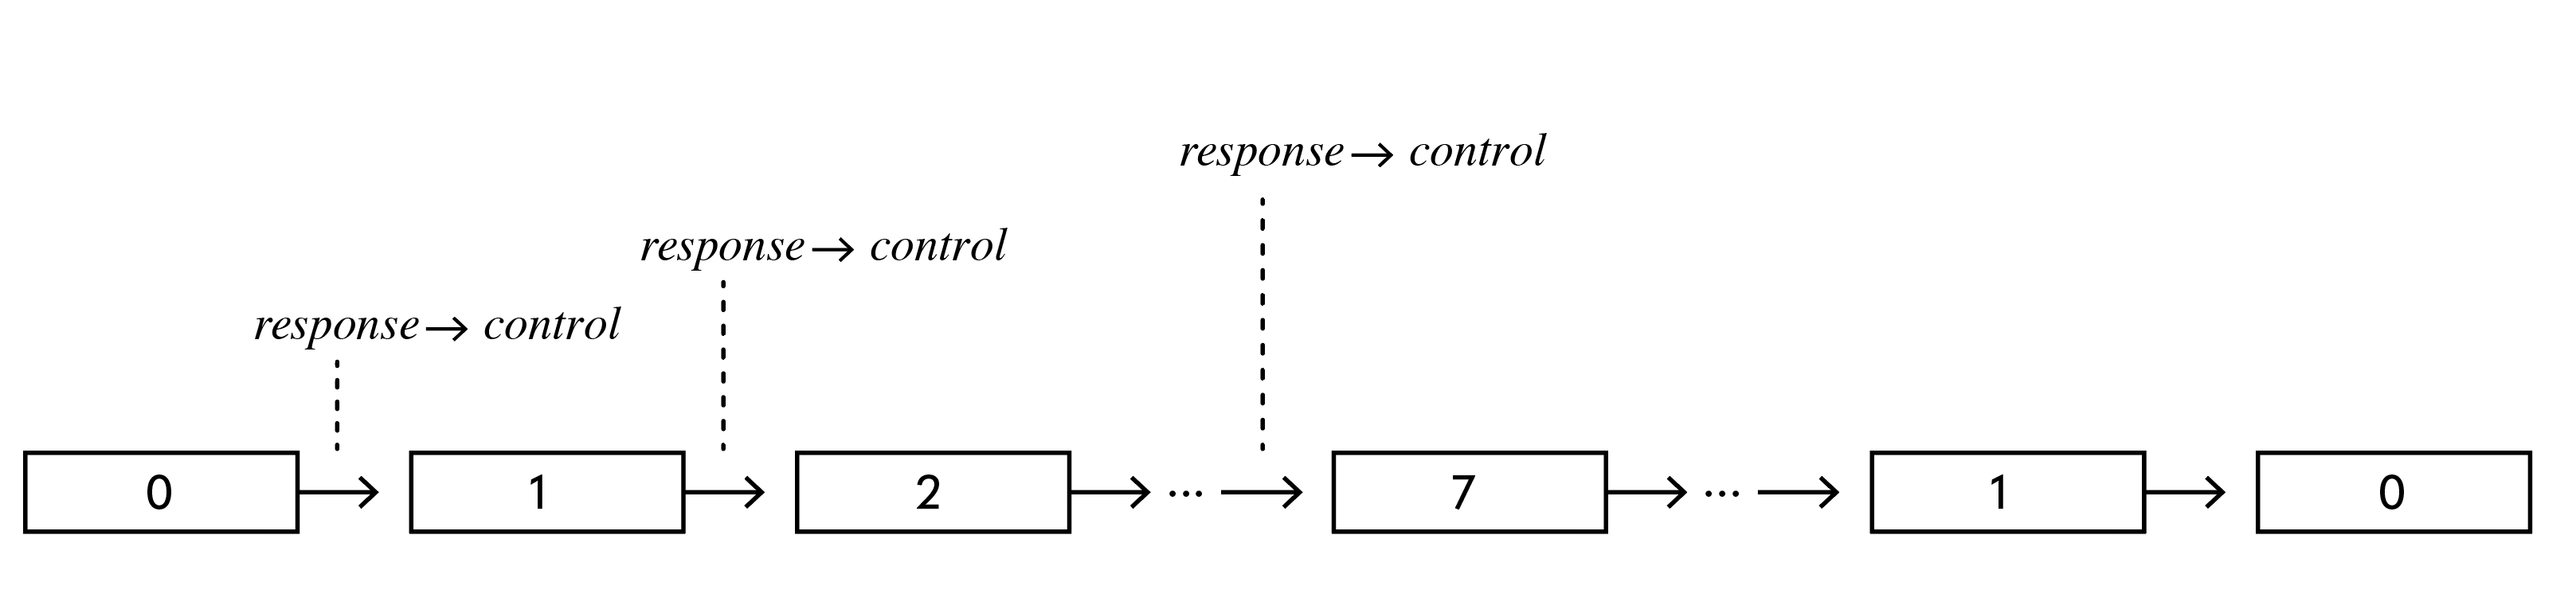
\includegraphics[width=15cm]{img/nerai_fs.png}
  \caption{《Familiar / Strange》のねらい}
  \label{fig:nerai_fs_in_discussion}
\end{figure}

実際に、シーンの遷移に伴い\textit{response}の関係性が喚起される様子が確認された。
最初、グー、チョキ、パーの形を作ったり(参加者2)、手を握りしめたり、開いたり(参加者4)をしていたが、シーンが切り替わると、次第に指ごとに別々に動かすようになった。そのとき、「どれがどの場所なんだろう[...]っていうのを確認していた」(参加者1)、「指の位置がどういうふうに対応しているのかを確かめている」(参加者4)
というように、対応関係の確認を行なっていたことがわかる。これは、自分自身の動きではないトランジションによって、画面の中の手指と自分自身の対応関係が自明なものではなくなったことを示していると考える。

さらにシーン7では、バネ状の形を動かす上で最も動きを繊細に捉えることのできる縦方向に手指を動かすことを通して「気持ちよさ」を経験する、\textit{control}とみられる関係性が確認された。体験者2は、指の動きが先端と付け根の動きだけを追従した形に変化したシーン4から、さらにその動きが縦軸に拘束されたシーン5への変化を通して、ピアノを弾くときのように指を一本一本上下に動かすようになり、シーン7になってもその動きを続けている中で、手指を素早く動かしていても反応して動くことに「気持ちいい」と語っていた。また、参加者4はこの形状が画面の変化が最も大きいことから「気持ちいい動きをしてもらうことだけを考えてた」といって振り返っていた。

しかし、シーン7においては\textit{control}と思われる関係性が確認された一方で、そこに至るまでのシーンでは\textit{control}の関係にはほとんど至らなかった。参加者は、「どれがどの場所なんだろう」といった確認をしていたが、それ以上に何か目的意識を持って身体を動かしていたというようなコメントは少ない。しかし、目的意識を見出していた参加者は、変換された手指の形状に対して何かしらの「見立て」をしていた。参加者4は、指が縦方向の動きのみに拘束されてパタパタと上下する形になったときに、「ピアノの演奏」のような身体感覚を想起していた。また参加者2は、シーン2や4をみて「植物か触角か、イソギンチャクみたいな感じ」に見立てると言ったように、「頭の中で既視感を作って」体験していたと振り返る。そうした見立てがなかなかできないシーンについては、「見たことない形のものだと[...]どうその曲線で遊ぶのかを見つけるのがなかなか大変」だったと語った。もし、見立てが可能な変換が行われていれば、この段階であっても\textit{control}の関係が生じていた可能性がある。

% 「見立て」は形に起因する見立ても存在するが、参加者4が身体の動きから「ピアノ」を連想していたように、過去に体験したことのあるような身体動作がこの場所で再演されることを通して、デジャヴのような感覚を引き起こす、「運動の見立て」の可能性も存在する。このように「見立て」が可能であることが、今後体験の中で目的意識や注意を自分で作って体験することにつながるのではないかと考える。

% また、最初の手指の形状からのトランジションによって親和性が失われていくことが確認された一方で、それ以降に親和性が失われていくような関係が芽生えてはいなかったのではないかと考えられる。参加者は作品の意図を知らされていないが、参加者2は、まさに「親和性」という言葉を用いて次のように体験を振り返っていた。
% \begin{quote}
%   ここら辺からちょっと違和感というか、親和性を確かめてたのに、その親和性から離れてく感じがしてた。今の自分の手と、こっち側の手の連動はしてるんだけど、離れている。自分の手じゃなくなる。
% \end{quote}
% そしてシーン7では「親和性」については諦めて、「身体的なところからは離れ」た存在となっていたことを振り返っていた。
% \begin{quote}
%   ここら辺からちょっと結構激しく手を動かし始めてた。[...]動きの精度を見てる。親和性はもう諦めて、動きの精度みたいなことを、よりシステムチックに見ちゃってる。身体的なところからは離れている、これはもう完全に。
% \end{quote}
% また、参加者4がシーン7において「気持ちいい動きをしてもらう」と語っていたことからも、自分の身体を動かしているというよりは、自分自身の身体ではないものを外から操っているような関係として認識していることが示唆される。そのため、体験の中で形状が変わった手指に対しても「まさに自分自身の身体である」と感じるような感覚が訪れ、それがトランジションによって崩壊する、といった違和感は現れない。実際、参加者4は度々「何も考えてなかった」瞬間があったことを振り返った。指がバネ状に積み重なっていくシーン6から7の遷移、そして手指の形にまた戻ってくるシーン1からシーン0への遷移の際である。このことから、すべてのトランジションが違和感を生み、ひいては意識的な試行を生むことに寄与するわけではないと考えられる。

加えて、作品のねらいとしたことがほとんど実現しなかった参加者もいた。
参加者3は最初、フレームを取るようなジェスチャーをしてトラッキングができていることを確かめていた。しかし手の形が変化し、異なる形状になっても「こうやってしたら(両手を開いて親指と人差し指をつなげ、三角形を作る)くっつくのかな」「(指を交差させて)こうやってやったら変わるのかな」と、「形を作る」ことに目的意識を抱いて体験していた。しかし、思うように形が作れないことから「反応がない」と感じられ、「飽きていた」とコメントしている。参加者3においてトランジションに伴う違和感が喚起されなかったのは、最初から「形を作る」ということに対して強い目的意識を抱いていたからではないかと考える。ジェスチャーを「入力」したはずなのに、何か意味を持った形が現れなかったことから「反応がない」と認識したのではないか。このことを踏まえると、この作品の体験においては、\textit{control}しようとすることだけに意識的になるだけではなく、グラフィックの変化に合わせて身体の動作を変化させていく必要があるのではないかと考えられる。

\section{Relation}
この作品におけるねらいは、ボールの操作やマトに当てるといった目的意識が起点となって意識的な試行が引き出され、その目的を達成するための技量を身につけることで一体感が生起することであった。またこの作品では、手そのもの、手とボール、ボールとマト、というように、段階的に緻密な運動の制御が求められることで、一体感(\textit{intimacy})が高まるのではないかと考えた。

\begin{figure}[H]
  \centering
  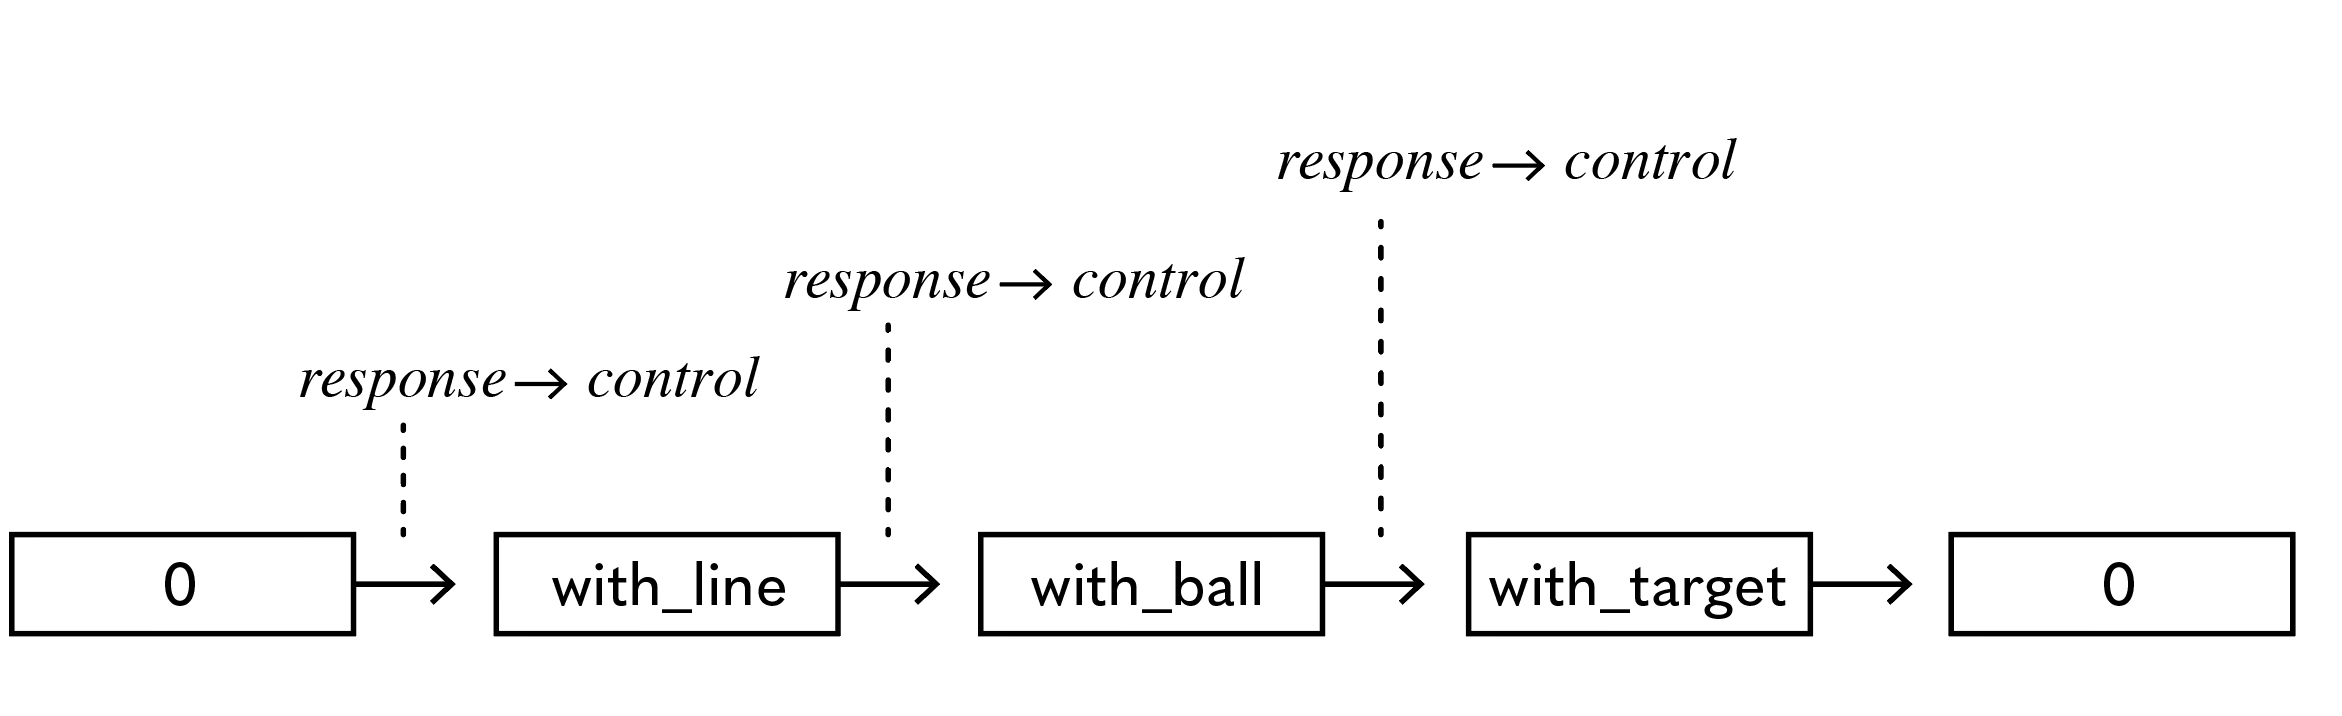
\includegraphics[width=15cm]{img/nerai_rl.png}
  \caption{《Relation》のねらい}
  \label{fig:nerai_rl_in_discussion}
\end{figure}

結果、体験の途中で目的が変化することは確認されたが、「マトにボールを当てる」という目的に対して十分な技量を身につけた参加者は現れず、インタビューから一体感(\textit{intimacy})が生じたと取れるような発言は得られなかった。
《Relation》において最初、いずれの参加者もマトの存在や役割に気づかず、しばらくは「左にボールがあったら右の方に移動させようとか、右にあったら左に移動させてみよう」(参加者1)、「どれぐらいの動きでどれぐらいバウンドするのか」、「ボールをちょっと滞在させたい」「ちょっとなだらかな面を作ろう」(参加者2)、「(ボールを画面外に)落とさないようにしよう」(参加者3)、「ボールを投げ上げよう」(参加者4)といった目的を見出していた。そして、途中からマトの存在や役割に気づき、それ以降はいずれの参加者も「マトに当てる」ということを目的としていた。
しかしマトにボールが当たることはあっても、それは偶然であったり、随意であっても再現性が低く、「一体感」を感じられるほど器用に操れるようになった参加者はいなかった。
最後、全員が「マトに当てる」ということを目的としていたため、感想が「マトに当てられなかった」という経験が中心となったのではないかと考えた。

しかしこのことは、参加者が何を目的としているかに依存して、同じ構造であっても「一体感」を感じられる、あるいは感じられなくなることを示唆している。
先に触れたように、参加者の目的意識は、体験の中で次第に変化していた。目的が変化する中、参加者4は「気持ちよさ」の変化について語っていた。
\begin{quote}
  気持ちよさを感じるポイントは、ゲームを進めていく中で変化していった[...]最初は「球を上げる」っていう目標になって、それを達成する気持ちよさがあった。それを超えて、次の目標が見つかったときには、マトに当てないと気持ちよくない。(参加者4)
\end{quote}
このことから、それまで「気持ちよさ」を感じていた対象であっても、目的意識の変化によって「一体感」は失われることもあるのではないかと考えられる。
また参加者2は、《Relation》において「投げるときの反応が鈍」く、手指の動きの遅延やトラッキングの精度に対して「イライラ」、「もどかしい」と振り返っていた。これは、同じシステムを用いている《Familiar / Strange》においては述べられることがなかった内容である。ボールをタイミングよく動かす必要のある《Relation》においては、そうした誤差が前景化し、手指に対する「一体感が低い」と感じられたのではないか。

% 一方で、トラッキングが途切れることの多かった参加者4は、トラッキングが途切れてしまったこと自体に不快感を示さなかった。
% こうしたことを踏まえると、体験における「もどかしさ」とは目的意識との関係にあり、トラッキングの精度やトラッキングの可否の問題ではないと考えられる。また、作品がどのように動くのかについて、実際の正しい振る舞いについて理解することよりも、何かしらの納得感が現れることの方が重要であることが示唆された。

% 一方で、参加者3は、手指の対応関係については認識していたと振り返ったが、体験の途中でそうした対応関係とは関係なく、手のひらを上に向けて掬い上げるような動きをしていた。慎重に画面の中で行われていることを観察した上で身体を動かすというよりは、自分の表現したいことを身振りでジェスチャーするような体験であったと言える。本作品は、手指の身体動作が全て認識されて動作するため、あらゆる動作を受け付けるという点で、探索をする上で適度に抽象的であると考える。ただしその一方で、慎重になることについては必ずしも必ずしも喚起出来ているわけではないということがわかった。しかし、その設計は慎重に行う必要がある。なぜなら注意を喚起する構造を設計することは、抽象度を高めることとトレードオフの関係となってしまうことがあるためである。

\section{Felsの議論の限界}
ここまで、Felsのembodimentの分類や\textit{intimacy}の生起という観点から、本作品が目指す「人馬一体感」を捉えようとしてきた。しかし、この作品において重要な体験でありながら、Felsの定義したカテゴリを用いるだけでは捉えきれなかったことがある。それは、手指の構造が変化することをきっかけに生じる、「身体動作の変化」である。本作品においては、体験中常に身体動作とグラフィックの連動性は担保されている。しかしながら、一度構造が変化すると自分の動きとの対応関係が曖昧になり、「動いてはいるが、自分が動かしている」という感覚が薄れていく。そして、改めて「どこがどのように対応しているのか」ということを動きの中で確認することを通して構造を把握し、再び「自分が動かしている」という感覚が芽生える。このとき、Felsのカテゴリで言えば「自分の動きによってそれが動いている」という点において\textit{control}の関係性であるということができるが、一方で「自分が動かしている」という感覚を得るためには確認の動作が必要であり、どのようにそれが振る舞うのかを理解して、それに合わせた身体の動かし方をする、すなわち対象に帰属(\textit{belonging})する必要がある。

この作品において生じている一体感とは、単に自分の思い通りに制御しようとするだけで生起するものではなく、作品の振る舞いを意識的に観察しながら、それに合わせて動作を変更しない限り起こらない。つまり、\textit{control}すると同時に\textit{belonging}することをなしには一体感が生起しない。実際、参加者3は「ジェスチャー」のような動きをしようとしたことに対して、作品からの影響を受けなかったことから一体感が生起しなかった。こうしたFelsの定義に収まりきらないところに、「人馬一体感」があるのではないか。


% 《Strange / Familiar》で見られた「どのように振る舞うのかを確かめる」、《Relation》に見られた「当てようとしても、思うように当たらない」といったときの関係性は、
% この作品における一体感を捉える上で重要であるが、それはFelsのいう\textit{control}にも、\textit{belonging}にも該当しない。

% このときの対象との関係性を、仮に「\textit{grasp}」とした。

% \section{新たに重要だと思われた指標}
% \subsection{見立て}
% 目的意識を抱いていた参加者は、何かしらの「見立て」をしていたことがわかった。参加者4は、指が縦方向の動きのみに拘束されてパタパタと上下する形になったときに、ピアノの演奏のような身体感覚を想起していた。また参加者2は、「頭の中で既視感を作って」体験していたと振り返る。こうした「見立て」が生じることは、体験する人がそこに目的意識を見出して、対象を捉えようとすることの表れと考えられる。

% 「見立て」は形に起因する見立ても存在するが、参加者4が身体の動きから「ピアノ」を連想していたように、過去に体験したことのあるような身体動作がこの場所で再演されることを通して、デジャヴのような感覚を引き起こす、「運動の見立て」の可能性も存在する。このように「見立て」が可能であることが、今後体験の中で目的意識や注意を自分で作って体験することにつながるのではないかと考える。

% \subsection{連動性の担保}
% 「思い通りに動く」とは「連動性が担保されていること」ではないか、という仮説が新たに生じた。「思い通り」という言葉は、相手に命令する立場からすると、期待している結果と実際の挙動が一致している際に生じるが、「control」の状態下での「思い通り」とは、参加者2が体験を振り返るコメントにもあるように、「トラッキングができて」いて、「時差を極力なくし」た動きが「自分の思い通りの動きになってくれる状態」、すなわち「連動性」ではないかということが示唆された。その上で、「Belonging:帰属感」のようなintimacyが生じるためには、その動きがさらに細かく制御できていることが重要ではないかと考えられる。

% \section{総括}
% 2つの作品では、それぞれ異なる性質の\textit{grasp}を喚起することが出来ていたことが明らかとなった。しかしその一方で、\textit{belonging}や\textit{control}といった関係性が芽生えていたと判断できるような状況が少なく、\textit{grasp}こそが親密さを高める要素として寄与していたのかについては、検証することが難しいと考えた。

% そこで、今後作品の体験を発展させる上で、\textit{control}や\textit{belonging}を発生させる可能性がある表現を、今回の分析を踏まえて列挙する。

% \begin{quote}
%   \begin{enumerate}
%     \item 「見立て」が可能な作品は、さらに目的意識を設定しやすく\textit{control}の関係性が芽生えることが考えられる。そのためには積極的に「見立て」が生じる状況を設計するというアプローチもありうるが、プロトタイピングでもあったように作品体験の複雑度を上げるような展開のさせ方も考えられる。今回の「Familiar / Strange」では、トランジションの過程でこの「見立て」が特に起こり得ず、目的意識を抱きづらい状況が続いていたことが課題として挙げられる。
%     \item 「マト」の存在は、全体的に強い目的意識を喚起させる表現となっていた一方で、体験者が目的意識を設定する余地をなくしてしまっていたことが考えられる。これは、「ゲーム性」を追及するのではない方法で目的意識をいかに設計していくのかという、遊びに関する議論とも接続する。前の要素とも関連するが、例えばオンスクリーン表現ではなく、フィジカルな表現で関係性の複雑度を上げるなど、注意を向ける対象の増やし方には検討の余地があると考える。
%     \item 体験の中で、抱いていた関心に対して試行しきることがないままに体験が終了していたことがあった。トランジションは作品の構造を示し、段階的に注意を向けることに寄与していた一方で、徐々に展開されてしまうことが集中を途切れさせる原因にもなっていたのではないかということが課題として挙げられる。
%   \end{enumerate}
% \end{quote}

\section{\textit{grasp}について}
そのため、「人馬一体感」を捉えるためには、「操作はしているが、自分が動かしているという感覚がない」という人と対象との関係を捉えるカテゴリが必要となると考えられる。そこで、本研究ではそのカテゴリを\textit{grasp}と名付けた。
graspは「把握」を意味する動詞であり、\textit{control}に向けて、対象の「思い通りにいかなさ」から影響を受けながら、折り合いをつけるために試行錯誤をしている状態である。本作品においてこの\textit{grasp}という関係性は、形が変化してから、身体動作を変化させていくまでのあいだに見られる。参加者1が《Relation》について、「ちょうどいい難易度で、所々面白かったな。[...]その面白かったなっていうのは、なかなかうまくいかんなっていう面白さ。[...]わかっちゃいるけど、うまくいかんなっていうような。」と語っているように、仕組みについては理解した上で、それでも自分の思うようにいかないような経験をしているとき、この\textit{grasp}が生じているのではないかと考えられる。

実際の体験の様子を分析した結果と、ここで新たに導入した\textit{grasp}を用いて体験を再び説明すると、作品での体験はそれぞれ次のように説明できる。

\begin{figure}[H]
  \centering
  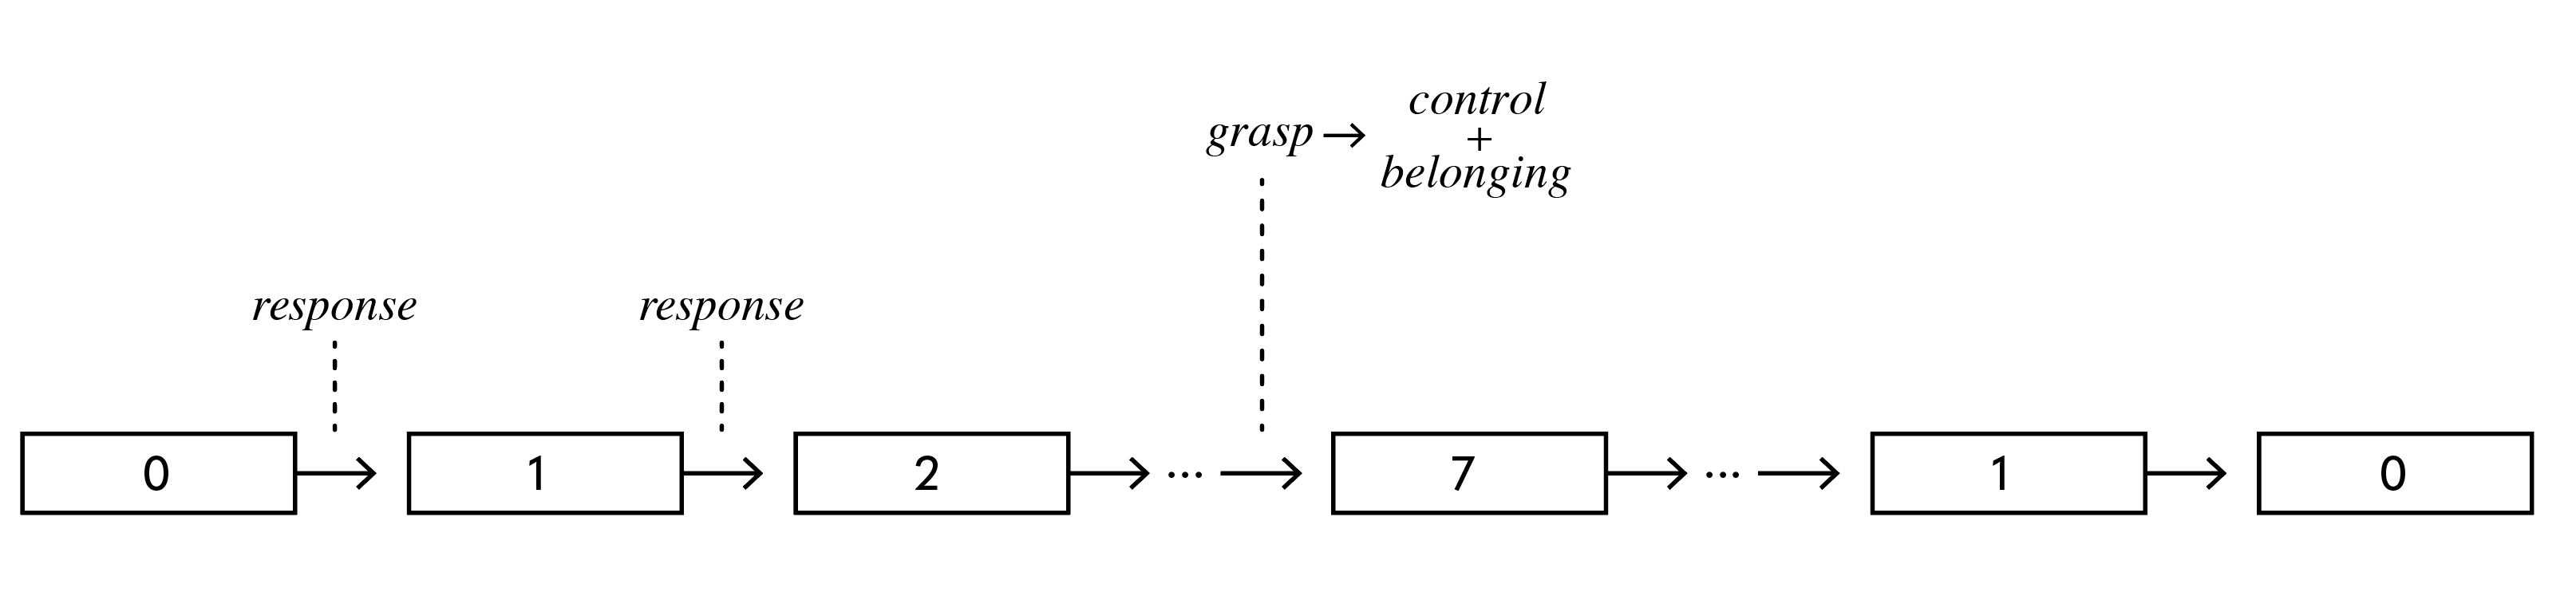
\includegraphics[width=15cm]{img/result_fs.png}
  \caption{\textit{grasp}を用いた《Familiar / Strange》の体験の説明}
  \label{fig:result_fs}
\end{figure}

《Familiar / Strange》においては、手指の変換だけでは「どこがどの指なのか」と確認することはあっても、それを踏まえて何か目的意識を抱くことは難しい。だが、シーン7のように複雑度が増し、動かすときに緻密な制御が求められるようになると、\textit{control}と取れるような経験があった。そして、この体験に至るためにはそれまでの\textit{response}を通して動きの仕組みについては理解していて、そうした経験を組み合わせることで、段階的にシーン7でその構造に合わせた動きができるよう、身体の動作が変化する\textit{grasp}の関係が間にあったと言える。また、そうした過程を経て一体感が生じるまでには、自分自身が身体の動かし方を変化させることが起きている。このことから、シーン7での一体感においては、\textit{control}に加えて\textit{belonging}も生じていると考えられる。

\begin{figure}[H]
  \centering
  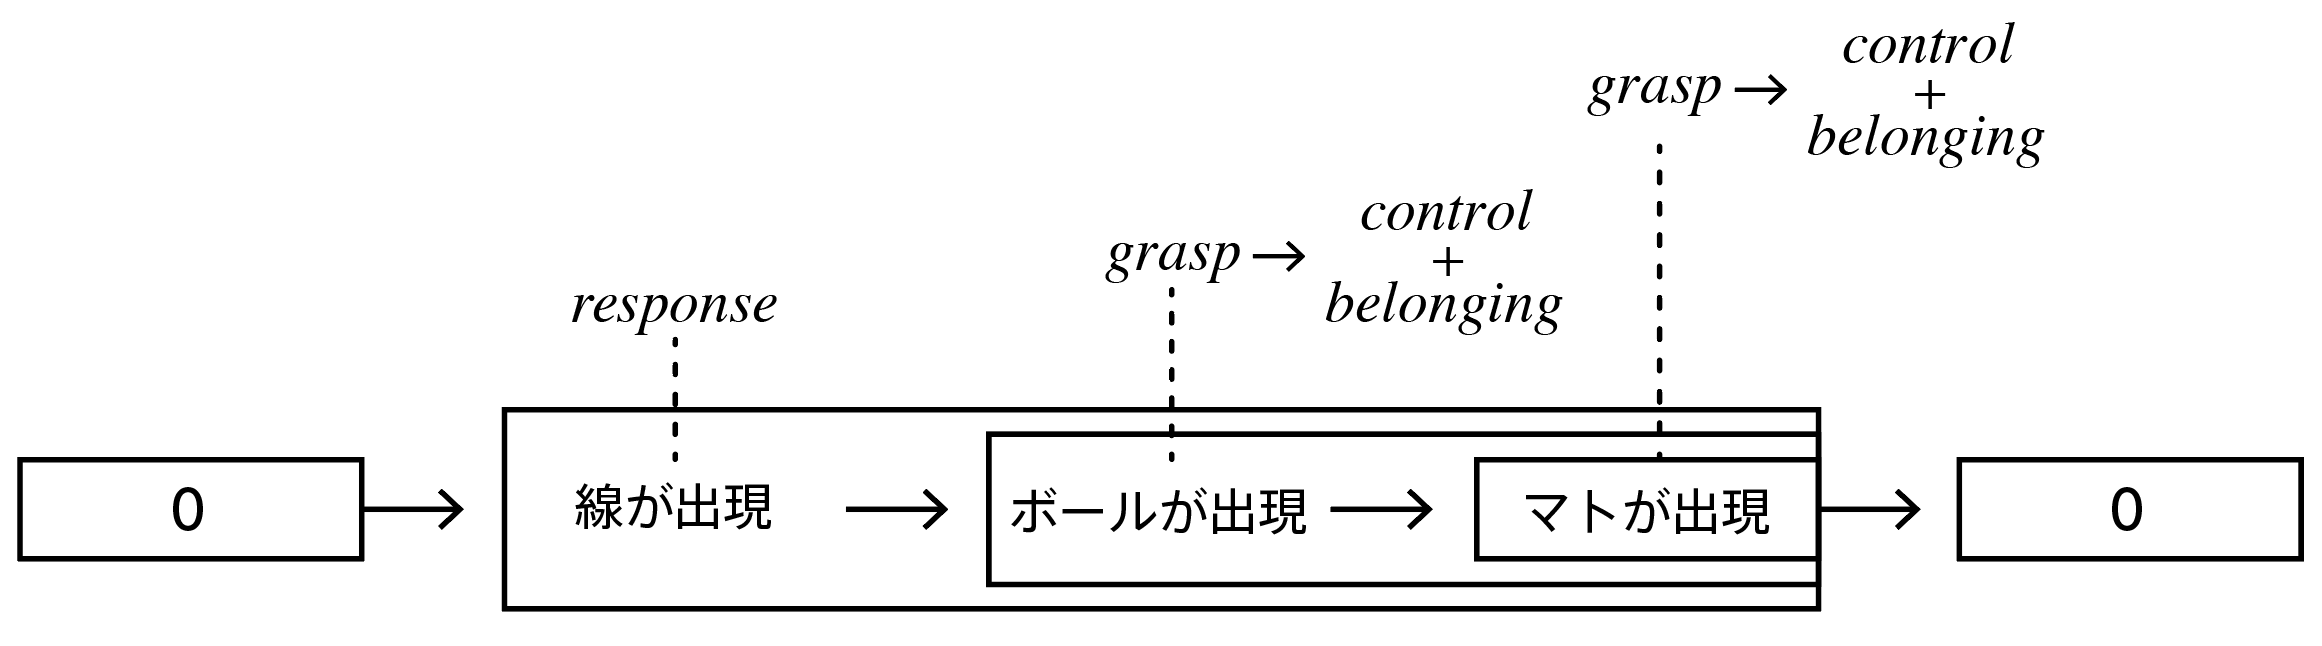
\includegraphics[width=15cm]{img/result_rl.png}
  \caption{\textit{grasp}を用いた《Relation》の体験の説明}
  \label{fig:result_rl}
\end{figure}

《Relation》においても、手指が変換していくだけでは目的意識を抱きづらく、\textit{response}はあっても\textit{control}の関係性には至ることが難しいのではないかと考えた。しかしボールが現れると、それを飛ばす、左右に転がすといった目的意識を抱くことや、

% \textit{grasp}とは例えば、ギターの習得過程において、弾きこなしたいフレーズを定め、それを達成するまでに試行錯誤をし、達成できるようになるまでの期間である。熟達した状態では、熟達する前とは違う視座でものごとを捉えられるようになり、また違う対象に注意が向くようになると、ギターと人との間に別の\textit{grasp}が芽生える。
% またあるいは、\textit{grasp}の過程で、対象と向き合い続ける過程の中でその解像度が高まり、当初目指していたこととは違うことに興味を抱く(セレンディピティ)ことでも、別の\textit{grasp}が芽生える。

% ここまで具体例を通してみてきたように、\textit{grasp}は、ギターと人との関係において一度だけ生じるのではなく、注目する対象が定まれば何度でも生じる。

% \textit{grasp}について、本研究では次のように定義する。

% \begin{quote}
%   \textbf{人と対象との関係の中で、人が対象の中に注意や目的意識を抱きながら、意識的に試行する期間}
% \end{quote}

% graspは「把握」を意味する動詞でもあるが、ここで「動作」ではなく「期間」とした。その理由は、「意識的に試行する」とき、同時にその結果を受けて気づきを得たり、その気づきをもとに新たな関心を抱くといった、単に自分が行為しているだけではなく、対象から影響を受けながら次の行為が決まってくるようなフィードバックループの構造があると考えるためである。「grasp=把握」という言葉についても、単に「ものを掴む」という意味だけでなく、「理解」の意味があることは、対象について一方向に働きかけているのではない様子が現れているのではないだろうか。


\newpage

%----------------------------------------------------------------------
% 5章 結論
%----------------------------------------------------------------------
\chapter{まとめ}
\label{matome}
本研究では、手指の異なる形状への変換から「身体の中の他者性」を経験させる表現を通してこの問いについて探索し、修士作品《Grasp(er)》を制作した。さらに、その体験を説明するものとして\textit{grasp}という概念を定義した。

本研究の狙いは、\textit{grasp}の観点から人と道具、機械、あるいは人体の中にある他者性との関係における「人馬一体」のような関係を捉えることである。そして、そうした関係性はどのようにして引き出すことができるのかを提示することである。

作品の分析を通して、本作品の表現は\textit{grasp}を喚起するものとして成功した側面もあったが、手指の変換構造については注意深くとらえない限り、認識が変化しないという体験の余地も残されていたことが明らかとなった。
また、この作品の体験を通して\textit{grasp}は生じていたものの、Felsの\textit{control}や、\textit{belonging}が生じていたと考えられる行為は少なかった。これは、作品の複雑さに起因する上限の可能性も考えられるため、\textit{grasp}がこうした関係性へと導くきっかけとなることの反証であったとは言いづらいが、同時に\textit{grasp}こそがこうした関係を喚起するものであったと結論づけるには、表現における課題が残り、検証に至らなかったと考える。

そこで、前節では今後に向けた表現の方向性として、体験者の意見や分析を通して得られた「見立て」や「複雑度」、「モーフィング表現についての再検討」が重要であると考える。

\section{今後の展望}
(それぞれ引用元を示す)

本節では、今回の研究や作品に反映することができなかったが、今後この概念をより発展させていくにあたり、論じていく必要があると考える2つの論点について整理する。1つは、青木淳による「原っぱと遊園地」、もうひとつは、ミゲル・シカールの遊び論に関する議論である。

\subsection{「原っぱと遊園地」}
建築家の青木淳は、建築においてそこで行われることをあらかじめ決定されているような空間を「遊園地」とし、一方で行われることで空間が作られていくような空間を「原っぱ」と呼び、分類している。

\begin{quote}
  ともかく、廃校になった機能主義的小学校の空間は、ちょうど原っぱのように、人間にそれ に対するかかわり方の自由を与える。 原っぱとは、つまり空き地である。 宅地が造成され区画 される。これは人工的な営みである。 塀が築かれ、土地の形がきちんと確定される。一度は土地が均され雑草が刈り取られる。 そこまで行って、なにかの理由で、放置される。時間が経過して、 セイタカアワダチソウなどの雑草が、背丈ほど伸びてくる。そして、原っぱができ上がる。 更地というだけでは、原っぱではない。放置後の、適切な度合いの自然の遂行を必要とする。 
  廃校になった牛込原町小学校は、原っぱと同じく、人間の感覚とは一度は切れた決定ルールによって生成し、しかしその決定ルールが根拠を失った空間だったのである。そうして、偶然に、そこで人がつくることと、与えられる空間の規定力の対等が実現されていたのである。  
\end{quote}

こうした「原っぱ」的な空間においては、そこにいる人が目的設定をした上で注意を向ける余地が生まれやすい。これは建築という空間設計の話だけではなく、\textit{grasp}の生起を目指したプロダクトや体験を設計する上で重要な設計論であるととらえている。

\subsection{シカールの「ふざけた遊び」}
しかしこうした「原っぱ」的なプロダクトに対して、本研究が期待するような関わり方が生起するためには、メディアアーティストの久保田が「使いやすさ」を志向することではなく、「使いたさ」を志向することの重要性を説くように、「強い目的意識」が生じることが重要である。

\begin{quote}
  楽器は、リアルタイムに音を生成、コントロールするための道具である。そのインターフェイスの使いやすさが重要になるのはいうまでもない。 しかし、ピアノのインターフェイスは「はじめての人にも使えるように」あるいは「一目でわかるように」デザインされているだろうか?ギターは?トランペットやサックスの場合は?いずれの楽器も、 はじめての人にとっては音を出すだけでも四苦八苦の、使いにくい道具である。にもかかわらず、人はそんな使いにくい楽器に対して時間をかけてじっくりと向き合い、日々練習を重ね、少しずつスキルを向上させながら美しい調べを自在に奏でる夢を見る。そうした営みを支えているのは、人々の願いやビジョンである。(中略)「使いやすさ」のためにも、何よりもまず「使いたい」という願望が必要である。「どうやってやるか」ということよりも「何をやるか」のほうが先に来る。 豊富な機能を生かすも殺すもインターフェイス次第であることは間違いないが、その豊富な機能を使いたいと思えなければしょうがない。考えてみれば当然だ。 携帯電話のテンキーによる文字入力が良い例だ。何も工夫していないものが、結局は一番使いやすいインターフェイスになっている。重要なのは、表面的な改良ではなく、大きさや重さ、速度といった基本的な要目だ。妙な工夫をするよりもむしろ、シンプルであればあるほどスキルが活躍する余地が生まれる。ワンタッチで具体的なインターフェイスよりも、システマティックで抽象的なインターフェイスのほうが、多様な使用法とアウトプットを生み出すことができる。その名人芸と形容したくなるほどのスキルを生み出しているのは、人々の欲望だ。ここでも、欲望さえあれば、指が勝手に動いていく。技術革新の速度はそれなりに速いのかもしれないが、その気になった人間の適応力や柔軟性による変化の速度はもっと速い。人間の可能性は、底知れない。
\end{quote}

しかし、こうした目的意識の生起については、自発的に発生するものもあれば、コミュニティの単位などで創発する場合もあるのではないかと考えられる。

こうした創発について述べるのは、ミゲル・シカールによる遊び論で語られる、「ふざけた遊び」の性質を持った遊び心の発露であろう。

\begin{quote}
  遊びは存在のためのポータブルな道具である。ゲームに代表されるような遊びの「形式」よりも、「世界のうちに存在するモードの一種」としての遊び、つまり人間が人間としてあるあり方のひとつとしての遊びである。遊びは文脈に依存する。これは遊びが、物や環境やテクノロジーや人などからなる、その都度の「文脈」を使うかたちで生じるということだ。シカールの考えでは、もともと遊びのためにデザインされたものであるはずのゲームのルールですら、その本来の目的を無視して流用してしまうのが、遊び心という態度であり、遊びという「人間存在のモード」なのだ。  
\end{quote}

本研究が着目した\textit{grasp}のコンセプトは、こうした人間の感情の発露を期待する。その意味で、誰もが同じようにそれに価値を見出すような、一般的な利便性よりも、属人的な楽しさを志向したアプローチであると言えるだろう。今後は、これらの議論と関連付けながら、本研究において達成することが出来なかった、\textit{belonging}や\textit{control}の関係性を喚起することについて、さらなる検討を深めていくことを考えている。
\newpage


%----------------------------------------------------------------------
% 謝辞
%----------------------------------------------------------------------
\chapter*{謝辞}
清々しい気持ちでこのページを書いているつもりが、書いてみてようやく自分の至らない点や、自分自身まだわかりきっていない部分が露呈して、実際には軽く吐き気がしています。しかしそれらを整理して再構成するには時間があまりに足りないので、論文執筆を通して指導いただいたことをもとに、時々思い返しては自分自身で赤入れをしていこうと思います。\\
主査の桑久保 亮太教授、副査の平林 真実教授には、度重なるアドバイスと作品・論文の審査をしていただきました。概念を曖昧にして用いていた点についての指摘を受けて論点を整理していく中で、いっそう明確になりました。\\
主指導教員の小林 茂教授には、研究内容にかかわるアドバイスに加え、論文執筆に際してはパラグラフごとのまとまりとパラグラフ間のつながりについて、細かく指導していただきました。応えることのできなかった指摘も多いとは思いますが、教わった作法は今後しっかりと身体化(embodiment)させていきたいと思います。\\
小林ゼミの小南菜子さん、太向弘明さん、成瀬陽太さん、そして聴講の松井美緒さんには、素朴な疑問から鋭い指摘まで、同じ学生同士だからこその忖度のない、貴重な意見をたくさんいただきました。私は今年で卒業ですが、この経験をみなさんの研究活動に還元していくことができたらと思います。また合宿にもいきましょう\footnote{それと、論文執筆に追われていたため未遂に終わった忘年会をやりたいです。}。\\
最後に、インタビューにご協力いただいた皆様、展示の機会を設けてくださったFab Cafe Nagoya様、IAMAS22期生の皆様、そのほか多くの研究にご協力いただいた皆様\footnote{列挙したらキリがなく、ひとまとめにしてすみません。これを執筆している今、お世話になった人々が、走馬灯のように頭の中を駆け回っています。あなたのことを、忘れていません。お会いしたときに直接感謝を伝えさせてください。}に深く感謝申し上げます。

\addcontentsline{toc}{chapter}{謝辞}
\newpage

%----------------------------------------------------------------------
% 参考文献
%----------------------------------------------------------------------
% \input{contents/references.tex}
\bibliographystyle{sty/sieicej}
\bibliography{references}

%----------------------------------------------------------------------
% 付録
%----------------------------------------------------------------------
\newpage
\appendix
\include{Appendix_model}

\label{付録}
\chapter{付録}


\end{document}